% !TeX document-id = {20a758e9-3325-489d-88bb-4096b1ed6a15}
% !TeX spellcheck = en-US
% !TeX encoding = utf8
% !TeX program = pdflatex
% !BIB program = biber
% -*- coding:utf-8 mod:LaTeX -*-


% vv  scroll down to line 200 for content  vv


\let\ifdeutsch\iffalse

\let\ifenglish\iftrue


% EN: This file is loaded before the \documentclass command in the main document

% EN: The following package allows \\ at the title page
%     For more information see https://github.com/latextemplates/scientific-thesis-cover/issues/4
\RequirePackage{kvoptions-patch}

\ifenglish
  \PassOptionsToClass{numbers=noenddot}{scrbook}
\else
  %()Aus scrguide.pdf - der Dokumentation von KOMA-Script)
  %Nach DUDEN steht in Gliederungen, in denen ausschließlich arabische Ziffern für die Nummerierung
  %verwendet werden, am Ende der Gliederungsnummern kein abschließender Punkt
  %(siehe [DUD96, R3]). Wird hingegen innerhalb der Gliederung auch mit römischen Zahlen
  %oder Groß- oder Kleinbuchstaben gearbeitet, so steht am Ende aller Gliederungsnummern ein
  %abschließender Punkt (siehe [DUD96, R4])
  \PassOptionsToClass{numbers=autoendperiod}{scrbook}
\fi

% Warns about outdated packages and missing caption declarations
% See https://www.ctan.org/pkg/nag
\RequirePackage[l2tabu, orthodox]{nag}

%DE: Neue deutsche Trennmuster
%    Siehe http://www.ctan.org/pkg/dehyph-exptl und http://projekte.dante.de/Trennmuster/WebHome
%    Nur für pdflatex, nicht für lualatex
\RequirePackage{ifluatex}
\ifluatex
  % do not load anything
\else
  \ifdeutsch
    \RequirePackage[ngerman=ngerman-x-latest]{hyphsubst}
  \fi
\fi

\documentclass[
  %
  %ngerman, %%% Add if you write in German.
  %
  % fontsize=11pt is the standard
  a4paper,  % Standard format - only KOMAScript uses paper=a4 - https://tex.stackexchange.com/a/61044/9075
  twoside,  % we are optimizing for both screen and two-side printing. So the page numbers will jump, but the content is configured to stay in the middle (by using the geometry package)
  bibliography=totoc,
  %               idxtotoc,   %Index ins Inhaltsverzeichnis
  %               liststotoc, %List of X ins Inhaltsverzeichnis, mit liststotocnumbered werden die Abbildungsverzeichnisse nummeriert
  headsepline,
  cleardoublepage=empty,
  parskip=half,
  %               draft    % um zu sehen, wo noch nachgebessert werden muss - wichtig, da Bindungskorrektur mit drin
  draft=false
]{scrbook}
% !TeX encoding = utf8
% -*- coding:utf-8 mod:LaTeX -*-

% EN: This file includes basic packages and sets options. The order of package
%     loading is important

% DE: In dieser Datei werden zuerst die benoetigten Pakete eingebunden und
%     danach diverse Optionen gesetzt. Achtung Reihenfolge ist entscheidend!


% EN: Styleguide:
% - English comments are prefixed with "EN", German comments are prefixed with "DE"
% - Prefixed headings define the language for the subsequent paragraphs
% - It is tried to organize packages in blocks. Bocks are separated by two empty lines.

% DE: Styleguide:
%
% Ein sehr kleiner Styleguide. Packages werden in Blöcken organisiert.
% Zwischen zwei Blöcken sind 2 Leerzeilen!


% EN: Enable copy and paste of text from the PDF
%     Only required for pdflatex. It "just works" in the case of lualatex.
%     mmap enables mathematical symbols, but does not work with the newtx font set
%     See: https://tex.stackexchange.com/a/64457/9075
%     Other solutions outlined at http://goemonx.blogspot.de/2012/01/pdflatex-ligaturen-und-copynpaste.html and http://tex.stackexchange.com/questions/4397/make-ligatures-in-linux-libertine-copyable-and-searchable
%     Trouble shooting outlined at https://tex.stackexchange.com/a/100618/9075

\ifluatex
\else
  \usepackage{cmap}
\fi


% EN: File encoding
% DE: Codierung
%     Wir sind im 21 Jahrhundert, utf-8 löst so viele Probleme.
%
% Mit UTF-8 funktionieren folgende Pakete nicht mehr. Bitte beachten!
%   * fancyvrb mit §
%   * easylist -> http://www.ctan.org/tex-archive/macros/latex/contrib/easylist/
\ifluatex
  % EN: See https://tex.stackexchange.com/a/158517/9075
  %     Not required, because of usage of fontspec package
  %\usepackage[utf8]{luainputenc}
\else
  \usepackage[utf8]{inputenc}
\fi


% DE: Parallelbetrieb tex4ht und pdflatex

\makeatletter
\@ifpackageloaded{tex4ht}{
  \def\iftex4ht{\iftrue}
}{
  \def\iftex4ht{\iffalse}
}
\makeatother


% EN: Mathematics
% DE: Mathematik
%
% DE: Viele Mathematik-Sachen. Siehe https://texdoc.net/pkg/amsmath
%
% EN: Options must be passed this way, otherwise it does not work with glossaries
% DE: fleqn (=Gleichungen linksbündig platzieren) funktioniert nicht direkt. Es muss noch ein Patch gemacht werden:
\PassOptionsToPackage{fleqn,leqno}{amsmath}
%
% DE: amsmath Muss nicht mehr geladen werden, da es von newtxmath automatisch geladen wird
% \usepackage{amsmath}


%% EN: Fonts
%% DE: Schriften
%%
%% !!! If you change the font, be sure that words such as "workflow" can
%% !!! still be copied from the PDF. If this is not the case, you have
%% !!! to use glyphtounicode. See comment at cmap package


% EN: Times Roman for all text
\ifluatex
  % source: Second proposed fix from the following answer: https://tex.stackexchange.com/a/394137
  \usepackage[no-math]{fontspec}
  \setmainfont{TeXGyreTermes-Regular}[
       BoldFont       = TeXGyreTermes-Bold ,
       ItalicFont     = TeXGyreTermes-Italic ,
       BoldItalicFont = TeXGyreTermes-BoldItalic,
       NFSSFamily     = ntxtlf]
  \setsansfont{TeX Gyre Heros Regular}[
       Scale=.9,
       BoldFont       = TeX Gyre Heros Bold,
       ItalicFont     = TeX Gyre Heros Italic,
       BoldItalicFont = TeX Gyre Heros BoldItalic]
  \setmonofont[StylisticSet={1,3},Scale=.9]{inconsolata}
  \RequirePackage{newtxmath}
\else
  \RequirePackage{newtxtext}
  \RequirePackage{newtxmath}
  % EN: looks good with times, but no equivalent for lualatex found,
  %     therefore replaced with inconsolata
  %\RequirePackage[zerostyle=b,scaled=.9]{newtxtt}
  \RequirePackage[varl,scaled=.9]{inconsolata}
\fi

% EN: Fallback font - if the subsequent font packages do not define a font (e.g., monospaced)
%     This is the modern package for "Computer Modern".
%     In case this gets activated, one has to switch from cmap package to glyphtounicode (in the case of pdflatex)
% DE: Fallback-Schriftart
%\usepackage[%
%    rm={oldstyle=false,proportional=true},%
%    sf={oldstyle=false,proportional=true},%
%    tt={oldstyle=false,proportional=true,variable=true},%
%    qt=false%
%]{cfr-lm}

% EN: Headings are typset in Helvetica (which is similar to Arial)
% DE: Schriftart fuer die Ueberschriften - ueberschreibt lmodern
%\usepackage[scaled=.95]{helvet}

% DE: Für Schreibschrift würde tun, muss aber nicht
%\usepackage{mathrsfs} %  \mathscr{ABC}

% EN: Font for the main text
% DE: Schriftart fuer den Fliesstext - ueberschreibt lmodern
%     Linux Libertine, siehe http://www.linuxlibertine.org/
%     Packageparamter [osf] = Minuskel-Ziffern
%     rm = libertine im Brottext, Linux Biolinum NICHT als serifenlose Schrift, sondern helvet (von oben) beibehalten
%\usepackage[rm]{libertine}

% EN: Alternative Font: Palantino. It is recommeded by Prof. Ludewig for German texts
% DE: Alternative Schriftart: Palantino, Packageparamter [osf] = Minuskel-Ziffern
%     Bitte nur in deutschen Texten
%\usepackage{mathpazo} %ftp://ftp.dante.de/tex-archive/fonts/mathpazo/ - Tipp aus DE-TEX-FAQ 8.2.1

% DE: Schriftart fuer Programmcode - ueberschreibt lmodern
%     Falls auskommentiert, wird die Standardschriftart lmodern genommen
%     Fuer schreibmaschinenartige Schluesselwoerter in den Listings - geht bei alten Installationen nicht, da einige Fontshapes (<>=) fehlen
%\usepackage[scaled=.92]{luximono}
%\usepackage{courier}
% DE: BeraMono als Typewriter-Schrift, Tipp von http://tex.stackexchange.com/a/71346/9075
%\usepackage[scaled=0.83]{beramono}

% EN: backticks (`) are rendered as such in verbatim environments.
%     See following links for details:
%     - https://tex.stackexchange.com/a/341057/9075
%     - https://tex.stackexchange.com/a/47451/9075
%     - https://tex.stackexchange.com/a/166791/9075
\usepackage{upquote}

% DE: Symbole
%
%\usepackage[geometry]{ifsym} % \BigSquare
%\usepackage{mathabx}
%\usepackage{stmaryrd} %fuer \ovee, \owedge, \otimes
%\usepackage{marvosym} %fuer \Writinghand %patched to not redefine \Rightarrow
%\usepackage{mathrsfs} %mittels \mathscr{} schoenen geschwungenen Buchstaben erzeugen
%\usepackage{calrsfs} %\mathcal{} ein bisserl dickeren buchstaben erzeugen - sieht net so gut aus.
%durch mathpazo ist das schon definiert

%
%\usepackage{amssymb}

% EN: For \texttrademark{}
\usepackage{textcomp}

% EN: name-clashes von marvosym und mathabx vermeiden:
\def\delsym#1{%
  %  \expandafter\let\expandafter\origsym\expandafter=\csname#1\endcsname
  %  \expandafter\let\csname orig#1\endcsname=\origsym
  \expandafter\let\csname#1\endcsname=\relax
}

%\usepackage{pifont}
%\usepackage{bbding}
%\delsym{Asterisk}
%\delsym{Sun}\delsym{Mercury}\delsym{Venus}\delsym{Earth}\delsym{Mars}
%\delsym{Jupiter}\delsym{Saturn}\delsym{Uranus}\delsym{Neptune}
%\delsym{Pluto}\delsym{Aries}\delsym{Taurus}\delsym{Gemini}
%\delsym{Rightarrow}
%\usepackage{mathabx} - Ueberschreibt leider zu viel - und die \le-Zeichen usw. sehen nicht gut aus!


% EN: Modern font encoding
%     Has to be loaded AFTER any font packages. See https://tex.stackexchange.com/a/2869/9075.
\ifluatex
\else
  \usepackage[T1]{fontenc}
\fi
%


% EN: Character protrusion and font expansion. See http://www.ctan.org/tex-archive/macros/latex/contrib/microtype/
% DE: Optischer Randausgleich und Grauwertkorrektur

\usepackage[
  babel=true, % EN: Enable language-specific kerning. Take language-settings from the languge of the current document (see Section 6 of microtype.pdf)
  expansion=alltext,
  protrusion=alltext-nott, % EN: Ensure that at listings, there is no change at the margin of the listing
  final % EN: Always enable microtype, even if in draft mode. This helps finding bad boxes quickly.
        %     In the standard configuration, this template is always in the final mode, so this option only makes a difference if "pros" use the draft mode
]{microtype}


% EN: \texttt{test -- test} keeps the "--" as "--" (and does not convert it to an en dash)
\DisableLigatures{encoding = T1, family = tt* }

% DE: fuer microtype
% DE: tracking=true muss als Parameter des microtype-packages mitgegeben werden
% DE: Deaktiviert, da dies bei Algorithmen seltsam aussieht

%\DeclareMicrotypeSet*[tracking]{my}{ font = */*/*/sc/* }%
%\SetTracking{ encoding = *, shape = sc }{ 45 }
% DE: Hier wird festgelegt,
%     dass alle Passagen in Kapitälchen automatisch leicht
%     gesperrt werden.
%     Quelle: http://homepage.ruhr-uni-bochum.de/Georg.Verweyen/pakete.html
%    Deaktiviert, da sonst "BPEL", "BPMN" usw. wirklich komisch aussehen.
%     Macht wohl nur bei geisteswissenschaftlichen Arbeiten Sinn.


% EN: amsmath teaks


% EN: Fixes bugs in AMS math
%     Corrently conflicts with unicode-math
% \usepackage{mathtools}

%\numberwithin{equation}{section}
%\renewcommand{\theequation}{\thesection.\Roman{equation}}

% EN: work-around ams-math problem with align and 9 -> 10. Does not work with glossaries, No visual changes.
%\addtolength\mathindent{1em}


% EN: For theorems, replacement for amsthm
\usepackage[amsmath,hyperref]{ntheorem}
\theorempreskipamount 2ex plus1ex minus0.5ex
\theorempostskipamount 2ex plus1ex minus0.5ex
\theoremstyle{break}
\newtheorem{definition}{Definition}[section]


% CTAN: https://ctan.org/pkg/lccaps
% Doc: http://texdoc.net/pkg/lccaps
%
% Required for DE/EN \initialism
\usepackage{lccaps}


% EN: Defintion of colors. Argument "hyperref" is not used as we do not want to change border colors of links: Links are not colored anymore.
% DE: Farbdefinitionen
\usepackage[dvipsnames]{xcolor}


% EN: Required for custom acronyms/glossaries style.
%     Left aligned Columns in tables with fixed width.
%     See http://tex.stackexchange.com/questions/91566/syntax-similar-to-centering-for-right-and-left
\usepackage{ragged2e}


% DE: Wichtig, ansonsten erscheint "No room for a new \write"
\usepackage{scrwfile}


% EN: Support for language-specific hyphenation
% DE: Neue deutsche Rechtschreibung und Literatur statt "Literature"
%     Die folgende Einstellung ist der Nachfolger von ngerman.sty
\ifdeutsch
  % DE: letzte Sprache ist default, Einbindung von "american" ermöglicht \begin{otherlanguage}{amercian}...\end{otherlanguage} oder \foreignlanguage{american}{Text in American}
  %     Siehe auch http://tex.stackexchange.com/a/50638/9075
  \usepackage[american,main=ngerman]{babel}
  % Ein "abstract" ist eine "Kurzfassung", keine "Zusammenfassung"
  \addto\captionsngerman{%
    \renewcommand\abstractname{Kurzfassung}%
  }
  \ifluatex
    % EN: conditionally disable ligatures. See https://github.com/latextemplates/scientific-thesis-template/issues/54
    %     for a discussion
    \usepackage[ngerman]{selnolig}
  \fi
\else
  % EN: Set English as language and allow to write hyphenated"=words
  %     `american`, `english` and `USenglish` are synonyms for babel package (according to https://tex.stackexchange.com/questions/12775/babel-english-american-usenglish).
  %      "english" has to go last to set it as default language
  \usepackage[english]{babel}
  % EN: Hint by http://tex.stackexchange.com/a/321066/9075 -> enable "= as dashes
  \addto\extrasenglish{\languageshorthands{ngerman}\useshorthands{"}}
  \ifluatex
    % EN: conditionally disable ligatures. See https://github.com/latextemplates/scientific-thesis-template/issues/54
    %     for a discussion
    \usepackage[english]{selnolig}
  \fi
\fi
%


% EN: For easy quotations: \enquote{text}
%     This package is very smart when nesting is applied, otherwise textcmds (see below) provides a shorter command
%     Note that this package results in a warning when it is loaded before minted (actually fvextra).
% DE: Anführungszeichen
%     Zitate in \enquote{...} setzen, dann werden automatisch die richtigen Anführungszeichen verwendet.
%     Dieses package erzeugt eine Warnung, wenn es vor minted (genauer fvextra) geladen wird.
\usepackage{csquotes}


% EN: For even easier quotations: \qq{text}.
%     Is not smart in the case of nesting, but good enough for the most cases
\usepackage{textcmds}
\ifdeutsch
  % EN: German quotes are different. So do not use the English quotes, but the ones provided by the csquotes package.
  \renewcommand{\qq}[1]{\enquote{#1}}
\fi


% EN: extended enumarations
% DE: erweitertes Enumerate
\usepackage{paralist}


% DE: Gestaltung der Kopf- und Fußteilen

\usepackage[automark]{scrlayer-scrpage}

\automark[section]{chapter}
\setkomafont{pageheadfoot}{\normalfont\sffamily}
\setkomafont{pagenumber}{\normalfont\sffamily}

% DE: funktioniert nicht: Alle Linien sind hier weg
%\setheadsepline[.4pt]{.4pt}


% DE: Intelligentes Leerzeichen um hinter Abkürzungen die richtigen Abstände zu erhalten, auch leere.
%     Siehe commands.tex \gq{}
\usepackage{xspace}
% DE: Macht \xspace und \enquote kompatibel
\makeatletter
\xspaceaddexceptions{\grqq \grq \csq@qclose@i \} }
\makeatother


\newcommand{\eg}{e.\,g.,\ }
\newcommand{\ie}{i.\,e.,\ }


% EN: introduce \powerset - hint by http://matheplanet.com/matheplanet/nuke/html/viewtopic.php?topic=136492&post_id=997377
\DeclareFontFamily{U}{MnSymbolC}{}
\DeclareSymbolFont{MnSyC}{U}{MnSymbolC}{m}{n}
\DeclareFontShape{U}{MnSymbolC}{m}{n}{
  <-6>    MnSymbolC5
  <6-7>   MnSymbolC6
  <7-8>   MnSymbolC7
  <8-9>   MnSymbolC8
  <9-10>  MnSymbolC9
  <10-12> MnSymbolC10
  <12->   MnSymbolC12%
}{}
\DeclareMathSymbol{\powerset}{\mathord}{MnSyC}{180}


% EN: Package for the appendix
% DE: Anhang
\usepackage{appendix}
%[toc,page,title,header]
%


% EN: Graphics
% DE: Grafikeinbindungen
%
% EN: The parameter "pdftex" is not required
\usepackage{graphicx}
\graphicspath{{\getgraphicspath}}
\newcommand{\getgraphicspath}{graphics/}


% EN: Enables inclusion of SVG graphics - 1:1 approach
%    This is NOT the approach of https://ctan.org/pkg/svg-inkscape,
%     which allows text in SVG to be typeset using LaTeX
%     We just include the SVG as is.
\usepackage{epstopdf}
\epstopdfDeclareGraphicsRule{.svg}{pdf}{.pdf}{%
  inkscape -z -D --file=#1 --export-pdf=\OutputFile
}


% EN: Enables inclusion of SVG graphics - text-rendered-with-LaTeX-approach
%     This is the approach of https://ctan.org/pkg/svg-inkscape,
\newcommand{\executeiffilenewer}[3]{%
  \IfFileExists{#2}
  {
    %\message{file #2 exists}
    \ifnum\pdfstrcmp{\pdffilemoddate{#1}}%
      {\pdffilemoddate{#2}}>0%
      {\immediate\write18{#3}}
    \else
      {%\message{file up to date #2}
      }
    \fi%
  }{
    %\message{file #2 doesn't exist}
    %\message{argument: #3}
    %\immediate\write18{echo "test" > xoutput.txt}
    \immediate\write18{#3}
  }
}
\newcommand{\includesvg}[1]{%
  \executeiffilenewer{#1.svg}{#1.pdf}%
  {
    inkscape -z -D --file=\getgraphicspath#1.svg %
    --export-pdf=\getgraphicspath#1.pdf --export-latex}%
  \input{\getgraphicspath#1.pdf_tex}%
}


% EN: Enable typesetting values with SI units.
\ifdeutsch
  \usepackage[mode=text,group-four-digits]{siunitx}
  \sisetup{locale=DE}
\else
  \usepackage[mode=text,group-four-digits,group-separator={,}]{siunitx}
  \sisetup{locale=US}
\fi


% EN: Extensions for tables
% DE: Tabellenerweiterungen
\usepackage{array} %increases tex's buffer size and enables ``>'' in tablespecs
\usepackage{longtable}
\usepackage{dcolumn} %Aligning numbers by decimal points in table columns
\ifdeutsch
  \newcolumntype{d}[1]{D{.}{,}{#1}}
\else
  \newcolumntype{d}[1]{D{.}{.}{#1}}
\fi
\setlength{\extrarowheight}{1pt}


% DE: Eine Zelle, die sich über mehrere Zeilen erstreckt.
%     Siehe Beispieltabelle in Kapitel 2
\usepackage{multirow}


% DE: Fuer Tabellen mit Variablen Spaltenbreiten
%\usepackage{tabularx}
%\usepackage{tabulary}


% EN: Links behave as they should. Enables "\url{...}" for URL typesettings.
%     Allow URL breaks also at a hyphen, even though it might be confusing: Is the "-" part of the address or just a hyphen?
%     See https://tex.stackexchange.com/a/3034/9075.
% DE: Links verhalten sich so, wie sie sollen
%     Zeilenumbrüche bei URLs auch bei Bindestrichen erlauben, auch wenn es verwirrend sein könnte: Gehört der Bindestrich zur URL oder ist es ein Trennstrich?
%     Siehe https://tex.stackexchange.com/a/3034/9075.
\usepackage[hyphens]{url}
%
%  EN: When activated, use text font as url font, not the monospaced one.
%      For all options see https://tex.stackexchange.com/a/261435/9075.
% \urlstyle{same}
%
% EN: Hint by http://tex.stackexchange.com/a/10419/9075.
\makeatletter
\g@addto@macro{\UrlBreaks}{\UrlOrds}
\makeatother


% DE: Index über Begriffe, Abkürzungen
%\usepackage{makeidx} makeidx ist out -> http://xindy.sf.net verwenden


% DE: lustiger Hack fuer das Abkuerzungsverzeichnis
%     nach latex durchlauf folgendes ausfuehren
%     makeindex ausarbeitung.nlo -s nomencl.ist -o ausarbeitung.nls
%     danach nochmal latex
%\usepackage{nomencl}
%    \let\abk\nomenclature %Deutsche Ueberschrift setzen
%          \renewcommand{\nomname}{List of Abbreviations}
%        %Punkte zw. Abkuerzung und Erklaerung
%          \setlength{\nomlabelwidth}{.2\hsize}
%          \renewcommand{\nomlabel}[1]{#1 \dotfill}
%        %Zeilenabstaende verkleinern
%          \setlength{\nomitemsep}{-\parsep}
%    \makenomenclature


% EN: Logic for TeX - enables if-then-else in commands
% DE: Logik für TeX
%     FÜr if-then-else @ commands.tex
\usepackage{ifthen}


% EN: Code Listings
% DE: Listings
\usepackage{listings}
\lstset{language=XML,
  showstringspaces=false,
  extendedchars=true,
  basicstyle=\footnotesize\ttfamily,
  commentstyle=\slshape,
  % DE: Original: \rmfamily, damit werden die Strings im Quellcode hervorgehoben. Zusaetzlich evtl.: \scshape oder \rmfamily durch \ttfamily ersetzen. Dann sieht's aus, wie bei fancyvrb
  stringstyle=\ttfamily,
  breaklines=true,
  breakatwhitespace=true,
  % EN: alternative: fixed
  columns=flexible,
  numbers=left,
  numberstyle=\tiny,
  basewidth=.5em,
  xleftmargin=.5cm,
  % aboveskip=0mm, %DE: deaktivieren, falls man lstlistings direkt als floating object benutzt (\begin{lstlisting}[float,...])
  % belowskip=0mm, %DE: deaktivieren, falls man lstlistings direkt als floating object benutzt (\begin{lstlisting}[float,...])
  captionpos=b
}

\ifluatex
\else
  % EN: Enable UTF-8 support - see https://tex.stackexchange.com/q/419327/9075
  \usepackage{listingsutf8}
  \lstset{inputencoding=utf8/latin1}
\fi

\ifdeutsch
  \renewcommand{\lstlistlistingname}{Verzeichnis der Listings}
\fi


% EN: Alternative to listings could be fancyvrb. Can be used together.
% DE: Alternative zu Listings ist fancyvrb. Kann auch beides gleichzeitig benutzt werden.
\usepackage{fancyvrb}
%
% EN: Font size for the normal text
% DE: Groesse fuer den Fliesstext. Falls deaktiviert: \normalsize
%\fvset{fontsize=\small}
%
% DE: Somit kann im Text ganz einfach §verbatim§ text gesetzt werden.
%     Disabled, because UTF-8 does not work any more and lualatex causes issues
%\DefineShortVerb{\§}
%
% EN: Shrink font size of listings
\RecustomVerbatimEnvironment{Verbatim}{Verbatim}{fontsize=\footnotesize}
\RecustomVerbatimCommand{\VerbatimInput}{VerbatimInput}{fontsize=\footnotesize}
%
% EN: Hack for fancyvrb based on http://newsgroups.derkeiler.com/Archive/Comp/comp.text.tex/2008-12/msg00075.html
%     Change of the solution: \Vref somehow collidated with cleveref/varioref as the output of \Vref{} was "Abschnitt 4.3 auf Seite 85"; therefore changed to \myVref -- so completely removed
%     See https://tex.stackexchange.com/q/132420/9075 for more information.
\newcommand{\Vlabel}[1]{\label[line]{#1}\hypertarget{#1}{}}
\newcommand{\lref}[1]{\hyperlink{#1}{\FancyVerbLineautorefname~\ref*{#1}}}


% EN: Tunings of captions for floats, listings, ...
% DE: Bildunterschriften bei floats genauso formatieren wie bei Listings
%     Anpassung wird unten bei den newfloat-Deklarationen vorgenommen
%     https://www.ctan.org/pkg/caption2 is superseeded by this package.
\usepackage{caption}


% EN: Provides rotating figures, where the PDF page is also turned
% DE: Ermoeglicht es, Abbildungen um 90 Grad zu drehen
%     Alternatives Paket: rotating Allerdings wird hier nur das Bild gedreht, während bei lscape auch die PDF-Seite gedreht wird.
%     Das Paket lscape dreht die Seite auch nicht
\usepackage{pdflscape}


% EN: Required for proper environments of fancyvrb and lstlistings
%    There is also the newfloat pacakge (recommended by minted), but we currently have no expericene with that
% DE: Wird für fancyvrb und für lstlistings verwendet
\usepackage{float}
%
% EN: Alternative to float package
%\usepackage{floatrow}
% DE: zustäzlich für den Paramter [H] = Floats WIRKLICH da wo sie deklariert wurden paltzieren - ganz ohne Kompromisse
%     floatrow ist der Nachfolger von float
%     Allerdings macht floatrow in manchen Konstellationen Probleme. Deshalb ist das Paket deaktiviert.
%
% EN: See http://www.tex.ac.uk/cgi-bin/texfaq2html?label=floats
% DE: floats IMMER nach einer Referenzierung platzieren
%\usepackage{flafter}


% EN: Put footnotes below floats
%     Source: https://tex.stackexchange.com/a/32993/9075
\usepackage{stfloats}
\fnbelowfloat


% EN: For nested figures
% DE: Fuer Abbildungen innerhalb von Abbildungen
%     Ersetzt die Pakete subfigure und subfig - siehe https://tex.stackexchange.com/a/13778/9075
\usepackage[hypcap=true]{subcaption}


% EN: Extended support for footnotes
% DE: Fußnoten
%
%\usepackage{dblfnote}  %Zweispaltige Fußnoten
%
% Keine hochgestellten Ziffern in der Fußnote (KOMA-Script-spezifisch):
%\deffootnote[1.5em]{0pt}{1em}{\makebox[1.5em][l]{\bfseries\thefootnotemark}}
%
% Abstand zwischen Fußnoten vergrößern:
%\setlength{\footnotesep}{.85\baselineskip}
%
% EN: Following command disables the separting line of the footnote
% DE: Folgendes Kommando deaktiviert die Trennlinie zur Fußnote
%\renewcommand{\footnoterule}{}
%
\addtolength{\skip\footins}{\baselineskip} % Abstand Text <-> Fußnote
%
% Fußnoten immer ganz unten auf einer \raggedbottom-Seite
% fnpos kommt aus dem yafoot package
\usepackage{fnpos}
\makeFNbelow
\makeFNbottom


% EN: Variable page heights
% DE: Variable Seitenhöhen zulassen
\raggedbottom


% DE: Falls die Seitenzahl bei einer Referenz auf eine Abbildung nur dann angegeben werden soll,
%     falls sich die Abbildung nicht auf der selben Seite befindet...
\iftex4ht
  %tex4ht does not work well with vref, therefore we emulate vref behavior
  \newcommand{\vref}[1]{\ref{#1}}
\else
  \ifdeutsch
    \usepackage[ngerman]{varioref}
  \else
    \usepackage{varioref}
  \fi
\fi


% EN: More beautiful tables if one uses \toprule, \midrule, \bottomrule
% DE: Noch schoenere Tabellen als mit booktabs mit http://www.zvisionwelt.de/downloads.html
\usepackage{booktabs}
%
%\usepackage[section]{placeins}


% EN: Graphs and Automata
%
% TODO: Since version 3.0 (2013-10-01), it supports pdflatex via the auto-pst-pdf package
%       Requires -shell-escape
%\usepackage{gastex}


%\usepackage{multicol}

% DE: kollidiert mit diplomarbeit.sty
%\usepackage{setspace}


% DE: biblatex statt bibtex
\usepackage[
  backend       = biber, %biber does not work with 64x versions alternative: bibtex8
  %minalphanames only works with biber backend
  sortcites     = true,
  bibstyle      = numeric,
  citestyle     = numeric,
  giveninits    = false,
  useprefix     = false, %"von, van, etc." will be printed, too. See below.
  minnames      = 1,
  minalphanames = 3,
  maxalphanames = 4,
  maxbibnames   = 99,
  maxcitenames  = 2,
  natbib        = true,
  eprint        = true,
  url           = true,
  doi           = true,
  isbn          = true,
  backref       = false]{biblatex}

% enable more breaks at URLs. See https://tex.stackexchange.com/a/134281.
\setcounter{biburllcpenalty}{7000}
\setcounter{biburlucpenalty}{8000}

\bibliography{bibliography}
%\addbibresource[datatype=bibtex]{bibliography.bib}

%Do not put "vd" in the label, but put it at "\citeauthor"
%Source: http://tex.stackexchange.com/a/30277/9075
\makeatletter
\AtBeginDocument{\toggletrue{blx@useprefix}}
\AtBeginBibliography{\togglefalse{blx@useprefix}}
\makeatother

%Thin spaces between initials
%http://tex.stackexchange.com/a/11083/9075
\renewrobustcmd*{\bibinitdelim}{\,}

%Keep first and last name together in the bibliography
%http://tex.stackexchange.com/a/196192/9075
\renewcommand*\bibnamedelimc{\addnbspace}
\renewcommand*\bibnamedelimd{\addnbspace}

%Replace last "and" by comma in bibliography
%See http://tex.stackexchange.com/a/41532/9075
\AtBeginBibliography{%
  \renewcommand*{\finalnamedelim}{\addcomma\space}%
}

\DefineBibliographyStrings{ngerman}{
  backrefpage  = {zitiert auf S\adddot},
  backrefpages = {zitiert auf S\adddot},
  andothers    = {et\ \addabbrvspace al\adddot},
  %Tipp von http://www.mrunix.de/forums/showthread.php?64665-biblatex-Kann-%DCberschrift-vom-Inhaltsverzeichnis-nicht-%E4ndern&p=293656&viewfull=1#post293656
  bibliography = {Literaturverzeichnis}
}

% EN: enable hyperlinked author names when using \citeauthor
%     source: http://tex.stackexchange.com/a/75916/9075
\DeclareCiteCommand{\citeauthor}
{\boolfalse{citetracker}%
  \boolfalse{pagetracker}%
  \usebibmacro{prenote}}
{\ifciteindex
  {\indexnames{labelname}}
  {}%
  \printtext[bibhyperref]{\printnames{labelname}}}
{\multicitedelim}
{\usebibmacro{postnote}}

% EN: natbib compatibility
%\newcommand{\citep}[1]{\cite{#1}}
%\newcommand{\citet}[1]{\citeauthor{#1} \cite{#1}}
% EN: Beginning of sentence - analogous to cleveref - important for names such as "zur Muehlen"
%\newcommand{\Citep}[1]{\cite{#1}}
%\newcommand{\Citet}[1]{\Citeauthor{#1} \cite{#1}}

% DE: Blindtext. Paket "blindtext" ist fortgeschritterner als "lipsum" und kann auch Mathematik im Text (http://texblog.org/2011/02/26/generating-dummy-textblindtext-with-latex-for-testing/)
%     kantlipsum (https://www.ctan.org/tex-archive/macros/latex/contrib/kantlipsum) ist auch ganz nett, aber eben auch keine Mathematik
%     Wird verwendet, um etwas Text zu erzeugen, um eine volle Seite wegen Layout zu sehen.
\usepackage[math]{blindtext}


% EN: Make LaTeX logos available by commands. E.g., \lualatex
%     Disabled, because currently causes \not= already defined
%\usepackage{dtk-logos}

% quick replacement:
\newcommand{\LuaLaTeX}{Lua\LaTeX\xspace}
\newcommand{\lualatex}{\LuaLaTeX}

% DE: Neue Pakete bitte VOR hyperref einbinden. Insbesondere bei Verwendung des
%     Pakets "index" wichtig, da sonst die Referenzierung nicht funktioniert.
%     Für die Indizierung selbst ist unter http://xindy.sourceforge.net
%     ein gutes Tool zu erhalten.
%     Hier also neue packages einbinden.
% EN: Add new packages at this place.


% EN: Provides hyperlinks
%     Option "unicode" fixes umlauts in the PDF bookmarks - see https://tex.stackexchange.com/a/338770/9075
%
% DE: Erlaubt Hyperlinks im Dokument.
%     Alle Optionen nach \hypersetup verschoben, sonst crash
%     Siehe auch: "Praktisches LaTeX" - www.itp.uni-hannover.de/~kreutzm
\usepackage[unicode]{hyperref}


% EN: Define colors
% DE: Da es mit KOMA 3 und xcolor zu Problemen mit den global Options kommt MÜSSEN die Optionen so gesetzt werden.
%     Eigene Farbdefinitionen ohne die Namen des xcolor packages
\definecolor{darkblue}{rgb}{0,0,.5}
\definecolor{black}{rgb}{0,0,0}


% EN: Define color of links and more
\hypersetup{
  % have both title and number hyperlinking to content
  linktoc=all,
  bookmarksnumbered=true,
  bookmarksopen=true,
  bookmarksopenlevel=1,
  breaklinks=true,
  colorlinks=true,
  pdfstartview=Fit,
  pdfpagelayout=SinglePage, % DE: Alterntaive: TwoPageRight -- zweiseitige Darstellung: ungerade Seiten rechts im PDF-Viewer - siehe auch http://tex.stackexchange.com/a/21109/9075
  %pdfencoding=utf8, % EN: This is probably the same as passing the option "unicode" at \usepackage{hyperref}
  filecolor=black,
  urlcolor=black,
  linkcolor=black,
  citecolor=black
}


% EN: Abbreviations - has to be loaded after hyperref
% DE: Abkürzungsverzeichnis - muss nach hyperref geladen werden
%
% DE: siehe http://www.dickimaw-books.com/cgi-bin/faq.cgi?action=view&categorylabel=glossaries#glsnewwriteexceeded
\usepackage[acronym,indexonlyfirst,nomain]{glossaries}
\ifdeutsch
  \addto\captionsngerman % DE: siehe https://tex.stackexchange.com/a/154566
  {%
    \renewcommand*{\acronymname}{Abkürzungsverzeichnis}
  }
\else
  \renewcommand*{\acronymname}{List of Abbreviations}
\fi
\renewcommand*{\glsgroupskip}{}
%
% EN: Removed Glossarie as a table as a quick fix to get the template working again
%     See http://tex.stackexchange.com/questions/145579/how-to-print-acronyms-of-glossaries-into-a-table
%
\makenoidxglossaries


% EN: Extensions for references inside the document (\cref{fig:sample}, ...)
% DE: cleveref für cref statt autoref, da cleveref auch bei Definitionen funktioniert
\usepackage[capitalise,nameinlink,noabbrev]{cleveref}
\ifdeutsch
  \crefname{table}{Tabelle}{Tabellen}
  \Crefname{table}{Tabelle}{Tabellen}
  \crefname{figure}{\figurename}{\figurename}
  \Crefname{figure}{Abbildung}{Abbildungen}
  \crefname{equation}{Gleichung}{Gleichungen}
  \Crefname{equation}{Gleichung}{Gleichungen}
  \crefname{theorem}{Theorem}{Theoreme}
  \Crefname{theorem}{Theorem}{Theoreme}
  \crefname{listing}{\lstlistingname}{\lstlistingname}
  \Crefname{listing}{Listing}{Listings}
  \crefname{section}{Abschnitt}{Abschnitte}
  \Crefname{section}{Abschnitt}{Abschnitte}
  \crefname{paragraph}{Abschnitt}{Abschnitte}
  \Crefname{paragraph}{Abschnitt}{Abschnitte}
  \crefname{subparagraph}{Abschnitt}{Abschnitte}
  \Crefname{subparagraph}{Abschnitt}{Abschnitte}
\else
  \crefname{listing}{\lstlistingname}{\lstlistingname}
  \Crefname{listing}{Listing}{Listings}
\fi


% DE: Zur Darstellung von Algorithmen
%     Algorithm muss nach hyperref geladen werden
\usepackage[chapter]{algorithm}
\usepackage[]{algpseudocode}


% DE: Links auf Gleitumgebungen springen nicht zur Beschriftung,
%     Doc: http://mirror.ctan.org/tex-archive/macros/latex/contrib/oberdiek/hypcap.pdf
%     sondern zum Anfang der Gleitumgebung
\usepackage[all]{hypcap}


% DE: Deckblattstyle
%
\ifdeutsch
  \PassOptionsToPackage{language=german}{scientific-thesis-cover}
\else
  \PassOptionsToPackage{language=english}{scientific-thesis-cover}
\fi


% EN: Bugfixes packages
%\usepackage{fixltx2e} %Fuer neueste LaTeX-Installationen nicht mehr benoetigt - bereinigte einige Ungereimtheiten, die auf Grund von Rueckwaertskompatibilitaet beibahlten wurden.
%\usepackage{mparhack} %Fixt die Position von marginpars (die in DAs selten bis gar nicht gebraucht werden}
%\usepackage{ellipsis} %Fixt die Abstaende vor \ldots. Wird wohl auch nicht benoetigt.


% EN: Settings for captions of floats
% DE: Formatierung der Beschriftungen
%
\captionsetup{
  format=hang,
  labelfont=bf,
  justification=justified,
  %single line captions should be centered, multiline captions justified
  singlelinecheck=true
}


% EN: New float environments for listings and algorithms
%
% \floatstyle{ruled} % TODO: enabled or disabled causes no change - listings and algorithms are always ruled
%
\newfloat{Listing}{tbp}{code}[chapter]
\crefname{Listing}{Listing}{Listings}

\newfloat{Algorithmus}{tbp}{alg}[chapter]
\ifdeutsch
  \crefname{Algorithmus}{Algorithmus}{Algorithmus}
\else
  \crefname{Algorithmus}{Algorithm}{Algorithms}
  \floatname{Algorithmus}{Algorithm}
\fi



% EN: Various chapter styles
% DE: unterschiedliche Chapter-Styles
%     u.a. Paket fncychap

% Andere Kapitelueberschriften
% falls einem der Standard von KOMA nicht gefaellt...
% Falls man zurück zu KOMA moechte, dann muss jede der vier folgenden Moeglichkeiten deaktiviert sein.

%\usepackage[Sonny]{fncychap}

%\usepackage[Bjarne]{fncychap}

%\usepackage[Lenny]{fncychap}

%DE: Zur Aktivierung eines der folgenden Möglichkeiten ein Paar von "\iffalse" und "\fi" auskommentieren

\iffalse
  \usepackage[Bjarne]{fncychap}
  \ChNameVar{\Large\sf} \ChNumVar{\Huge} \ChTitleVar{\Large\sf}
  \ChRuleWidth{0.5pt} \ChNameUpperCase
\fi

\iffalse
  \usepackage[Rejne]{fncychap}
  \ChNameVar{\centering\Huge\rm\bfseries}
  \ChNumVar{\Huge}
  \ChTitleVar{\centering\Huge\rm}
  \ChNameUpperCase
  \ChTitleUpperCase
  \ChRuleWidth{1pt}
\fi

\iffalse
  \usepackage{fncychap}
  \ChNameUpperCase
  \ChTitleUpperCase
  \ChNameVar{\raggedright\normalsize} %\rm
  \ChNumVar{\bfseries\Large}
  \ChTitleVar{\raggedright\Huge}
  \ChRuleWidth{1pt}
\fi

\iffalse
  \usepackage[Bjornstrup]{fncychap}
  \ChNumVar{\fontsize{76}{80}\selectfont\sffamily\bfseries}
  \ChTitleVar{\raggedright\Large\sffamily\bfseries}
\fi

% EN: Complete different chapter style - self made

% Innen drin kann man dann noch zwischen
%   * serifenloser Schriftart (eingestellt)
%   * serifenhafter Schriftart (wenn kein zusaetzliches Kommando aktiviert ist) und
%   * Kapitälchen wählen
\iffalse
  \makeatletter
  %\def\thickhrulefill{\leavevmode \leaders \hrule height 1ex \hfill \kern \z@}

  %Fuer Kapitel mit Kapitelnummer
  \def\@makechapterhead#1{%
    \vspace*{10\p@}%
    {\parindent \z@ \raggedright \reset@font
      %Default-Schrift: Serifenhaft (gut fuer englische Dokumente)
      %A) Fuer serifenlose Schrift:
      \fontfamily{phv}\selectfont
      %B) Fuer Kapitaelchen:
      %\fontseries{m}\fontshape{sc}\selectfont
      %C) Fuer ganz "normale" Schrift:
      %\normalfont
      %
      \Large \@chapapp{} \thechapter
      \par\nobreak\vspace*{10\p@}%
      \interlinepenalty\@M
      {\Huge\bfseries\baselineskip3ex
        %Fuer Kapitaelchen folgende Zeile aktivieren:
        %\fontseries{m}\fontshape{sc}\selectfont
        #1\par\nobreak}
      \vspace*{10\p@}%
      \makebox[\textwidth]{\hrulefill}%    \hrulefill alone does not work
      \par\nobreak
      \vskip 40\p@
    }}

  %Fuer Kapitel ohne Kapitelnummer (z.B. Inhaltsverzeichnis)
  \def\@makeschapterhead#1{%
    \vspace*{10\p@}%
    {\parindent \z@ \raggedright \reset@font
      \normalfont \vphantom{\@chapapp{} \thechapter}
      \par\nobreak\vspace*{10\p@}%
      \interlinepenalty\@M
      {\Huge \bfseries %
        %Default-Schrift: Serifenhaft (gut fuer englische Dokumente)
        %A) Fuer serifenlose Schrift folgende Zeile aktivieren:
        \fontfamily{phv}\selectfont
        %B) Fuer Kapitaelchen folgende Zeile aktivieren:
        %\fontseries{m}\fontshape{sc}\selectfont
        #1\par\nobreak}
      \vspace*{10\p@}%
      \makebox[\textwidth]{\hrulefill}%    \hrulefill does not work
      \par\nobreak
      \vskip 40\p@
    }}
  %
  \makeatother
\fi


% DE: Minitoc-Einstellungen
%\dominitoc
%\renewcommand{\mtctitle}{Inhaltsverzeichnis dieses Kapitels}


% EN: Nicer paragraph line placement:
%     - Disable single lines at the start of a paragraph (Schusterjungen)
%     - Disable single lines at the end of a paragraph (Hurenkinder)
%     Normally, this is clubpenalty and widowpenalty, but using a package, it feels more non-hacky
\usepackage[all,defaultlines=3]{nowidow}
%
\displaywidowpenalty = 10000


% EN: Try to get rid of "overfull hbox" things and let text flow batter
%     See also
%       - http://groups.google.de/group/de.comp.text.tex/browse_thread/thread/f97da71d90442816/f5da290593fd647e?lnk=st&q=tolerance+emergencystretch&rnum=5&hl=de#f5da290593fd647e
%       - http://www.tex.ac.uk/cgi-bin/texfaq2html?label=overfull
\tolerance=2000
%
% EN: This could be increased to 20pt
\setlength{\emergencystretch}{3pt}
%
% EN: Suppress hbox warnings if less than 1pt
\setlength{\hfuzz}{1pt}


% EN: Fix names for algorithms in German
% DE: fuer algorithm.sty: - falls Deutsch und nicht Englisch.
\ifdeutsch
  \floatname{algorithm}{Algorithmus}
  \renewcommand{\listalgorithmname}{Verzeichnis der Algorithmen}
\fi


% EN: The euro sign
% DE: Das Euro Zeichen
%     Fuer Palatino (mathpazo.sty): richtiges Euro-Zeichen
%     Alternative: \usepackage{eurosym}
\newcommand{\EUR}{\ppleuro}


% Float-placements - http://dcwww.camd.dtu.dk/~schiotz/comp/LatexTips/LatexTips.html#figplacement
% and http://people.cs.uu.nl/piet/floats/node1.html
\renewcommand{\topfraction}{0.85}
\renewcommand{\bottomfraction}{0.95}
\renewcommand{\textfraction}{0.1}
\renewcommand{\floatpagefraction}{0.75}
%\setcounter{totalnumber}{5}

% EN: ensure that floats covering a whole page are placed at the top of the page
%    see http://tex.stackexchange.com/a/28565/9075
\makeatletter
\setlength{\@fptop}{0pt}
\setlength{\@fpbot}{0pt plus 1fil}
\makeatother



% DE: Bei Gleichungen nur dann die Nummer zeigen, wenn die Gleichung auch referenziert wird
%     Funktioniert mit MiKTeX Stand 2012-01-13 nicht. Deshalb ist dieser Schalter deaktiviert.
%
%\mathtoolsset{showonlyrefs}


% EN: Margins
% DE: Ränder
%     Viele Moeglichkeiten, die Raender im Dokument einzustellen.
%
%     Satzspiegel neu berechnen. Dokumentation dazu ist in "scrguide.pdf" von KOMA-Skript zu finden
%     Optionen werden bei \documentclass[] in ausarbeitung.tex mitgegeben.
% \typearea[current]{current} %neu berechnen, da neue Schrift eingebunden

%\usepackage{a4}
%\usepackage{a4wide}
%\areaset{170mm}{277mm} %a4:29,7hochx21mbreit

%Wer die Masse direkt eingeben moechte:
%Bei diesem Beispiel wird die Regel nicht beachtet, dass der innere Rand halb so gross wie der aussere Rand und der obere Rand halb so gross wie der untere Rand sein sollte
%\usepackage[inner=2.5cm, outer=2.5cm, includefoot, top=3cm, bottom=1.5cm]{geometry}

% EN: Package geometry to enlarge on page
%
%     Normally, geometry should not be used as the typearea package calculates the margins perfectly for printing
%     However, we want better screen-readable documents where the content does not "jump"
%     Thus, we fix the margins left and right to the same value
%
%     Source: http://www.howtotex.com/tips-tricks/change-margins-of-a-single-page/
%
\usepackage[
  left=3cm,right=3cm,top=2.5cm,bottom=2.5cm,
  headsep=18pt,
  footskip=30pt,
  includehead,
  includefoot
]{geometry}


% EN: Provides todo notes
% DE: schoene TODOs
\ifdeutsch
  \usepackage[colorinlistoftodos,ngerman]{todonotes}
\else
  \usepackage[colorinlistoftodos]{todonotes}
\fi
\setlength{\marginparwidth}{2,5cm}

\let\xtodo\todo
\renewcommand{\todo}[1]{\xtodo[inline,color=black!5]{#1}}
\newcommand{\utodo}[1]{\xtodo[inline,color=green!5]{#1}}
\newcommand{\itodo}[1]{\xtodo[inline]{#1}}


% EN: Enable footnotes in tables.
%     This package superseeds the 1997 package "footnote"
\usepackage{footnotehyper}
% TODO: The footnotehyper author recommends to enclose the respective area with \begin{savenotes} ... \end{savenotes}
\makesavenoteenv{tabular}
\makesavenoteenv{table}
% Reuse of footnotes, see http://tex.stackexchange.com/questions/10102/multiple-references-to-the-same-footnote-with-hyperref-support-is-there-a-bett
\crefformat{footnote}{#2\footnotemark[#1]#3}


% EN: pgfplots (optional if the ppackage is installed)
%     PGFPlots draws high-qual­ity func­tion plots in nor­mal or log­a­rith­mic scal­ing
\IfFileExists{pgfplots.sty}{
  \usepackage{pgfplots}
  % EN: highest version supported by overleaf as of 2018-03-16
  \pgfplotsset{compat=1.14}
}{}


% EN: pgfplotstable (optional if the ppackage is installed)
%     PGFPlots generates tables from csv files
\IfFileExists{pgfplotstable.sty}{
  \usepackage{pgfplotstable}
}{}


% EN: Package for creating graphics programmatically
\usepackage{tikz}


% EN: Package for creating uml diagramms
\usepackage{tikz-uml}


% EN: Forest: apgf/TikZ-based package for drawing linguistic trees - https://ctan.org/pkg/forest
\usepackage{forest}


% EN: Enable PlantUML listings in the environment "plantuml"
\IfFileExists{plantuml.sty}{
  \usepackage[output=latex]{plantuml}
}{}


% EN: Layout: bottoms of pages not aligned to each other
% DE: Der untere Rand darf "flattern"
\raggedbottom


% DE: Wie tief wird das Inhaltsverzeichnis aufgeschlüsselt
% 0 --\chapter
% 1 --\section % fuer kuerzeres Inhaltsverzeichnis verwenden - oder minitoc benutzen
% 2 --\subsection
% 3 --\subsubsection
% 4 --\paragraph
\setcounter{tocdepth}{1}


% EN: Fixes wrong spacing in the TOC.
%     Source: https://tex.stackexchange.com/a/33842/9075 -> comment by esdd
\RedeclareSectionCommand[tocnumwidth=2.8em]{section}


% DE: Angaben in die PDF-Infos uebernehmen
\makeatletter
\hypersetup{
  pdftitle={}, %Titel der Arbeit
  pdfauthor={}, %Author
  pdfkeywords={}, % CR-Klassifikation und ggf. weitere Stichworte
  pdfsubject={}
}
\makeatother


% EN: Higher compression of the output PDF
\pdfcompresslevel=9


% EN: Required for recent version of komascript, as some packges are not that compatible with KOMAScript as they should be
%     Has to be loaded at the *very* end, so we use "\AtEndPreamble" by etoolsbox
\usepackage{etoolbox}
\AtEndPreamble{\usepackage{scrhack}}


% EN: Provide tables over multiple pages
\usepackage{longtable}


% EN: Show LaTeX commands and their results in the document
%     Enables the command \PrintDemo
% See https://github.com/latextemplates/scientific-thesis-template/issues/82 for further discussion
\usepackage{latexdemo}


% DE: Fuer deutsche Texte: Weniger Silbentrennung, mehr Abstand zwischen den Woertern
\ifdeutsch
  \setlength{\emergencystretch}{3em} % Silbentrennung reduzieren durch mehr frei Raum zwischen den Worten
\fi



\usepackage[
  title={Trustworthiness of Synthetic Media in the Context of a Newscast}, % Do not forget to capitalize your title correctly, you may use the following page to help you: https://capitalizemytitle.com/
  author={Danilo Pejakovic},
  %orcid=0000-0000-0000-0000, % get your own ORCID via https://orcid.org/
  email={danilo.pejakovic@campus.lmu.de},
  type={Masterthesis},
  institute={Institute for Informatics}, % or other institute names - or just a plain string using {Demo\\Demo...}
  course={Mediainformatics},
  examiner={Prof.\ Dr.\ Sylvia Rothe, Christoph Weber},
  supervisor={Prof.\ Dr.\ Sylvia Rothe},
  startdate={October 4, 2023},
  enddate={April 4, 2024},
  % Falls keine Lizenz gewünscht wird bitte auf "none" setzen
  % Die Lizenz erlaubt es zu nichtkommerziellen Zwecken die Arbeit zu
  % vervielfältigen und Kopien zu machen. Dabei muss aber immer der Autor
  % angegeben werden. Eine kommerzielle Verwertung ist für den Autor
  % weiter möglich.
  copyright=ccbysa, % ccbysa, ccbynosa, cc0, none
  language=english
]{lmu-thesis-cover}

% Hier stehen alle Abkürzungen
% \newacronym{label}{abbrv}{long}
\newacronym{w2l}{W2L}{Wav2Lip}
\newacronym{ri}{RI}{Realism Index}
\newacronym{tts}{TTS}{text-to-speech}
\newacronym{t2i}{t2i}{text-to-image}
\newacronym{rvc}{RVC}{retrieval-based voice conversion}
\newacronym{v2v}{v2v}{voice-to-voice}
\newacronym{br}{BR}{Bayerischer Rundfunk}
\newacronym{sd}{SD}{Stable Diffusion}
\newacronym{hf}{HF}{HuggingFace.com}
\newacronym{lora}{LoRa}{low-rank adaptation}
\newacronym{ai}{AI}{Artificial Intelligence}
\newacronym{genai}{gen. AI}{generative Artificial Intelligence}
\newacronym{oss}{OSS}{open-source software}
\newacronym{dfl}{DFL}{DeepFaceLab}
\newacronym{fps}{fps}{frames per second}
\newacronym{oom}{OOM}{out-of-memory Error}
\newacronym{psm}{PSM}{Public Service Media}
\newacronym{dvt}{DVT}{Danilo's Voice Toolkit}
\newacronym{ae}{AE}{Adobe After Effects}
\newacronym{ue}{UE}{Unreal Engine}
\newacronym{prpro}{PrPro}{Adobe Premiere Pro}
\newacronym{gan}{GAN}{generative adverserial network}
\newacronym{saas}{SaaS}{software-as-a service}
\newacronym{hff}{HFF}{University for Television and Film Munich}
\newacronym{c2pa}{C2PA}{Coalition for Content Provenance and Authenticity}
\newacronym{rtvc}{RTVC}{Real Time Voice Cloning}
\newacronym{uvr}{UVR}{ultimate vocal remover}
\newacronym{auto1}{A 1111}{Automatic 1111}
\newacronym{nerf}{NeRF}{Neural Radiance Fields}
\newacronym{obs}{OBS}{Open Broadcaster Software}
\newacronym{dfl-dst}{dst}{destination}
\newacronym{dfl-src}{src}{source}
\newacronym{ldm}{LDM}{latent diffusion model}

\geometry{
  left=2.5cm,
  right=3.5cm,
  top=2cm,
  bottom=2cm
}

\makeindex

\begin{document}

\frontmatter
\pagenumbering{roman} % Seitennummerierung mit römischen Ziffern für den Vorspann
\setcounter{tocdepth}{2} % bis zur dritten Gliederungsebene Anzeigen



%tex4ht-Konvertierung verschönern
\iftex4ht
  % tell tex4ht to create picures also for formulas starting with '$'
  % WARNING: a tex4ht run now takes forever!
  \Configure{$}{\PicMath}{\EndPicMath}{}
  %$ % <- syntax highlighting fix for emacs
  \Css{body {text-align:justify;}}

  %conversion of .pdf to .png
  \Configure{graphics*}
  {pdf}
  {\Needs{"convert \csname Gin@base\endcsname.pdf
      \csname Gin@base\endcsname.png"}%
    \Picture[pict]{\csname Gin@base\endcsname.png}%
  }
\fi

%\VerbatimFootnotes %verbatim text in Fußnoten erlauben. Geht normalerweise nicht.

% DE: wird fuer Tabellen benötigt (z.B. >{centering\RBS}p{2.5cm} erzeugt einen zentrierten 2,5cm breiten Absatz in einer Tabelle
\newcommand{\RBS}{\let\\=\tabularnewline}

% EN: To avoid issues with Springer's \mathplus
%     See also http://tex.stackexchange.com/q/212644/9075
\providecommand\mathplus{+}

% DE: typoraphisch richtige Abkürzungen
\newcommand{\zB}{z.\,B.\xspace}
\newcommand{\bzw}{bzw.\xspace}
\newcommand{\usw}{usw.\xspace}
\renewcommand{\dh}{d.\,h.\xspace}

% EN: from hmks makros.tex - \indexify
\newcommand{\toindex}[1]{\index{#1}#1}

% DE: Tipp aus "The Comprehensive LaTeX Symbol List"
\newcommand{\dotcup}{\ensuremath{\,\mathaccent\cdot\cup\,}}

% DE: Anstatt $|x|$ $\abs{x}$ verwenden.
%     Die Betragsstriche skalieren automatisch, falls "x" etwas größer sein sollte...
\newcommand{\abs}[1]{\left\lvert#1\right\rvert}

% DE: für Zitate
\newcommand{\citeS}[2]{\cite[S.~#1]{#2}}
\newcommand{\citeSf}[2]{\cite[S.~#1\,f.]{#2}}
\newcommand{\citeSff}[2]{\cite[S.~#1\,ff.]{#2}}
\newcommand{\vgl}{vgl.\ }
\newcommand{\Vgl}{Vgl.\ }

% EN: For the algorithmic package
\newcommand{\commentchar}{\ensuremath{/\mkern-4mu/}}
\algrenewcommand{\algorithmiccomment}[1]{\hfill $\commentchar$ #1}

% DE: Seitengrößen - Gegen Schusterjungen und Hurenkinder...
\newcommand{\largepage}{\enlargethispage{\baselineskip}}
\newcommand{\shortpage}{\enlargethispage{-\baselineskip}}

\newcommand{\initialism}[1]{%
  \ifdeutsch%
    \textsc{#1}\xspace%
  \else%
    \textlcc{#1}\xspace%
  \fi%
}
\newcommand{\OMG}{\initialism{OMG}}
\newcommand{\BPEL}{\initialism{BPEL}}
\newcommand{\BPMN}{\initialism{BPMN}}
\newcommand{\UML}{\initialism{UML}}

%\pagenumbering{arabic}
\Coverpage
\Copyright
%Eigener Seitenstil fuer die Kurzfassung und das Inhaltsverzeichnis
\deftriplepagestyle{preamble}{}{}{}{}{}{\pagemark}
%Doku zu deftriplepagestyle: scrguide.pdf
\pagestyle{preamble}
\renewcommand*{\chapterpagestyle}{preamble}



%Kurzfassung / abstract
%auch im Stil vom Inhaltsverzeichnis

\section*{Abstract}

\todo{Short summary of the thesis. Here, the following questions should be answered:}
\todo{What is the specific problem addressed?}
\todo{What have you done?}
\todo{What did you find out?}
\todo{What are the implications on a larger scale?}
\todo{Should be around 0.5 pages. Not longer than 1 page.}

\cleardoublepage


% BEGIN: Verzeichnisse

\iftex4ht
\else
  \microtypesetup{protrusion=false}
\fi

%%%
% Literaturverzeichnis ins TOC mit aufnehmen, aber nur wenn nichts anderes mehr hilft!
% \addcontentsline{toc}{chapter}{Literaturverzeichnis}
%
% oder zB
%\addcontentsline{toc}{section}{Abkürzungsverzeichnis}
%
%%%

%Produce table of contents
%
%In case you have trouble with headings reaching into the page numbers, enable the following three lines.
%Hint by http://golatex.de/inhaltsverzeichnis-schreibt-ueber-rand-t3106.html
%
%\makeatletter
%\renewcommand{\@pnumwidth}{2em}
%\makeatother
%
\tableofcontents

% Bei einem ungünstigen Seitenumbruch im Inhaltsverzeichnis, kann dieser mit
% \addtocontents{toc}{\protect\newpage}
% an der passenden Stelle im Fließtext erzwungen werden.

\listoffigures
\listoftables


% Control List of Listings
\let\iflistings\iffalse
%Wird nur bei Verwendung von der lstlisting-Umgebung mit dem "caption"-Parameter benoetigt
%\lstlistoflistings
%ansonsten:
\iflistings
  \ifdeutsch
    \listof{Listing}{Verzeichnis der Listings}
  \else
    \listof{Listing}{List of Listings}
  \fi
\fi

% Control List of Algorithms
\let\ifalgorithms\iffalse
\ifalgorithms
  %mittels \newfloat wurde die Algorithmus-Gleitumgebung definiert.
  %Mit folgendem Befehl werden alle floats dieses Typs ausgegeben
  \ifdeutsch
    \listof{Algorithmus}{Verzeichnis der Algorithmen}
  \else
    \listof{Algorithmus}{List of Algorithms}
  \fi
  %\listofalgorithms %Ist nur für Algorithmen, die mittels \begin{algorithm} umschlossen werden, nötig
\fi

% Control Glossary
\let\ifglossary\iftrue
\ifglossary
  \printnoidxglossaries
\fi

\iftex4ht
\else
  %Optischen Randausgleich und Grauwertkorrektur wieder aktivieren
  \microtypesetup{protrusion=true}
\fi

% END: Verzeichnisse


% Headline and footline
\renewcommand*{\chapterpagestyle}{scrplain}
\pagestyle{scrheadings}
\pagestyle{scrheadings}
\ihead[]{}
\chead[]{}
\ohead[]{\headmark}
\cfoot[]{}
\ofoot[\usekomafont{pagenumber}\thepage]{\usekomafont{pagenumber}\thepage}
\ifoot[]{}


%% vv  scroll down for content  vv %%

\mainmatter

%%%%%%%%%%%%%%%%%%%%%%%%%%%%%%%%%%%%%%%%%%%%%%%%%%%%%%%%%%%%%%%%%%%%%%%%%%%%%%
%
% Main content starts here
%
%%%%%%%%%%%%%%%%%%%%%%%%%%%%%%%%%%%%%%%%%%%%%%%%%%%%%%%%%%%%%%%%%%%%%%%%%%%%%%


\chapter{Introduction}
\label{chap:introduction}


%\todo{P1.1. What is the large scope of the problem?}
\begin{figure}[h]
  \centering
  \begin{subfigure}[b]{0.4\textwidth}
    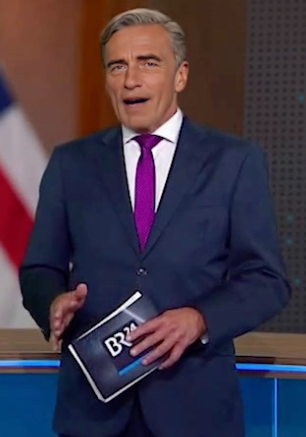
\includegraphics[width=\textwidth]{./graphics/images/scheider-real.png}
  \end{subfigure}
  \hfill
  \begin{subfigure}[b]{0.4\textwidth}
    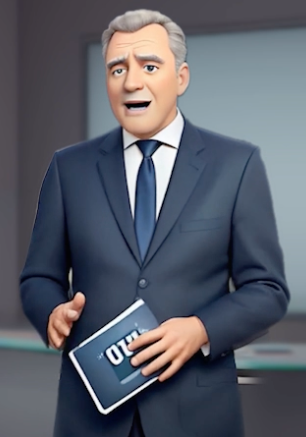
\includegraphics[width=\textwidth]{./graphics/images/scheider-sd.png}
  \end{subfigure}
  \caption{A TV news anchor: real and synthetic adaptation}
  \label{fig:scheider-real-sd}
\end{figure}
\begin{quotation}
"Sophiscitcated AI systems are increasingly everywhere. [...] However, 2023 will likely prove to be a particularly critical moment in the history of AI" \citet{arguedasAutomatingDemocracyGenerative2023}.
\end{quotation}
This paper and corresponding study are being conducted in the very year 2023. As the previously quoted authors state, we might be experiencing a tippping point in AI development, as more and more tools become available to a broader user base. These developments are tightly linked to the rise of OpenAi's ChatGPT and other, widely adopted technologies like \gls{sd} based \gls{t2i} generators. An output example of how future media could  be produced is depicted in figure \ref{fig:scheider-real-sd}. A more detailed description about the relevant technologies will be provided in section \ref{chap:background} \nameref{chap:background}. \\
Current AI tools are often referred to as \gls{genai}: "Generative AI is an umbrella term used for AI systems that can generate new forms of data, often by applying machine learning to large quantities of training data" \citet{arguedasAutomatingDemocracyGenerative2023}. One could extend this definition with the following: Besides just generating new forms of data, \gls{genai} can be used to augment, reduce, manipulate and mix real data with the generated data in such a form, that it is impossible to distinguish between real, syntheticly generated (fake) data, or anything in between that spectrum. \\
%\todo{P1.2. What is the specific problem?}
In the context of media production and and media distribution the developments of \gls{genai} open up an important discussion about trust and credibility. Legitimate media, has always been using synthetic content for various purposes. One can just think of animated explainatory videos or other infographics. The difference is, that most illustrations made it quite clear, that these images were illustrations. This has now changed as generated images and videos can look perfectly authentic and real. At the same time these technologies are open to be used by anyone, sparking fear of fake news. Therefore the question for legitimate media outlets remains, of how synthetic content will be recieved among the audience. Additionally, just the term "AI" sparks criticism. These effects on audience, their mitigation, and at the same time, education of the broader public about technologic advancements are very interesting topics for media producers and outlets. Since the developments are quite recent only few research examples exist.

% Second Paragraph
% CORE MESSAGE OF THIS PARAGRAPH:
%\todo{P2.1. The second paragraph should be about what have others been doing}
For the sake of completeness, these discussions are not entirely new: So called DeepFakes (blend word of Deep learning and Fake News) have been around quite some time. First research papers like Facebook's 2014 DeepFace \cite{taigmanDeepFaceClosingGap2014} or the Face2Face approach by \citet{thiesFace2FaceRealtimeFace2020} date back to the year 2016. It took some time until the research gained traction among a the broader audience, but at latest in 2017, in the form of DeepFake pornography or revenge porn, DeepFakes hit the broader public \cite{coleAIAssistedFakePorn2017}. 
Or as \citet{westerlundEmergenceDeepfakeTechnology2019a} puts it: "After the introduction of celebrity porn deepfakes to Reddit by one user in late 2017, it only took a few months for a newly founded deepfake hobbyist community to reach 90,000 members".
Quickly afterwards discussions arose about the implications of these technologies in regards to the spread of fake news.
It took some time until the fears came true. \\
In the meantime DeepFakes remained very problematic present within pornography but also in entertainment and educational content: Jordan Peele Faked Obama (2018 \cite{vincentWatchJordanPeele2018}), Channel 4 emitted a fake Queen Elizabeth (2020 \cite{DeepfakeQueenDeliver2020}) and VFX Artist Chris Ume went viral with Tom Cruise Fakes (2021 \cite{vincentTomCruiseDeepfake2021}). \\
Despite the proliferation of payed and \gls{oss} solutions for faceswaps, like \gls{dfl} (2019) or the InsightFace Inswapper (2023), there are only a few known cases, where this technology has been used for one singular disinformation video with larger consequences. However, it goes without saying, that the effect in social networks, under the radar of public control, might be much bigger. Some studies about these hypothesis will be featured in section \ref{chap:rel-work}. \\
The first mentioning of a trust dissolving DeepFake happened in 2022: Fake news of President Zelensky surfaced (Figure \ref{fig:zelensky-deepfake}), where the fake demanded soldiers to lay down their weapons. Although the russian creators of the video later disputed their creation as "satire" this was certainly not clear within the original video. For what had been feared for quite some time had become reality. The technology had been used in a political context, probably the first time in history also in an armed conflict. Some might say it had been weaponized. Although the Video seemed to have no concrete consequences for the soldiers, its role in psychological warfare can't be unseen.
\begin{figure}[h]
  \centering
  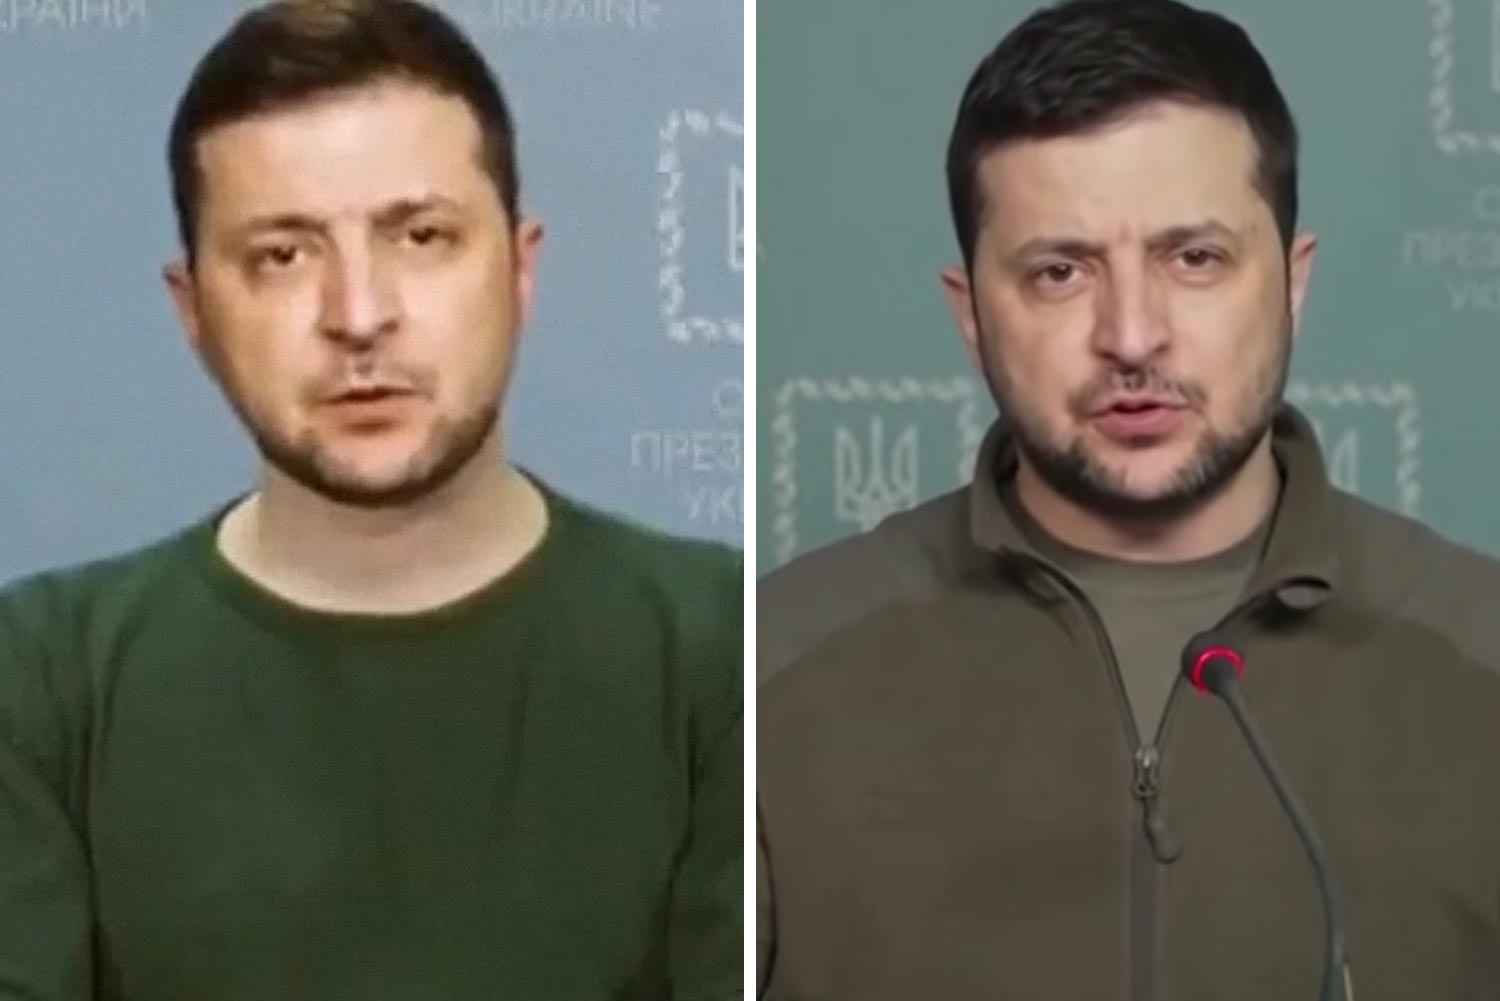
\includegraphics[width=0.5\textwidth]{./graphics/images/Zelensky.jpg}
  \caption{left: DeepFake of President Zelensky; right: real image of Zelensky \cite{universityofvirginiaZelenskyySurrenderHoax2022}}
  \label{fig:zelensky-deepfake}
\end{figure}

%\todo{P2.2. Why is the problem important? Why was this work carried out?}
Progressing in time, in the second half of 2022 several things changed in the space of AI tools. The aforementioned \textit{simple} faceswaps are now in good company in a growing toolbox of AI services: 
\begin{enumerate}
  \item Excellent AI voices cloning tools became available
  \item Text to image generation was released in summer 2022
  \item GPT-enabled Chat Applications was released end of 2022
\end{enumerate}
The latter is less relevant in the audio-visual content, but fuels the public opinion about A.I. tools as it is probably most widely adopted. The first two have drastically improved the quality and possibilities of how and what kind of synthetic media can be created. In the recent months there have been several reports about their use with increasing frequency: 
The examples of fake voices and faceswaps on social media in 2023 are innumerable and can be traced back to the availability of online services such as Resemble.ai or Elevenlabs. This also lead to several nefarious use cases: To name some examples in German context, in September 2023 a primetime news host was recreated with a fake voice in order to advertise dubious financial products (figure: \ref{fig:sievers-fake}). By using Elevenlabs' checking tool, one can quickly tell, that the voice was likely created with their software.(figure: \ref{fig:sievers-11labs}). 
\begin{figure}[h]
  \centering
  \begin{subfigure}[b]{0.45\textwidth}
    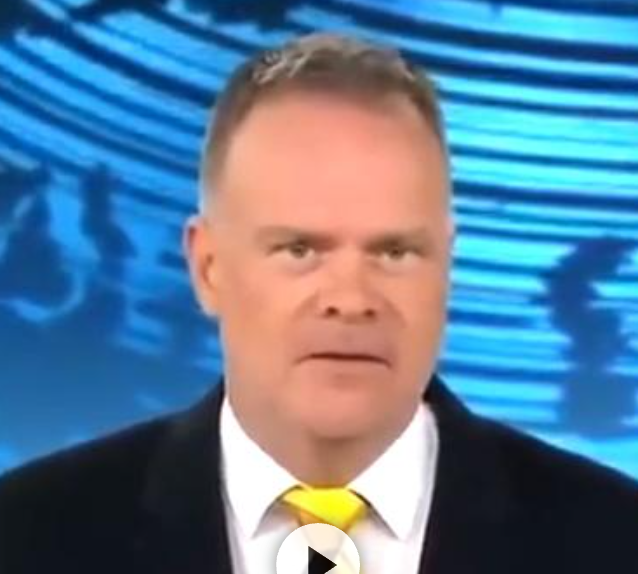
\includegraphics[width=\textwidth]{./graphics/images/sievers.png}
    \caption{fake of Christian Sievers \cite{zdfDeepfakeMitZDFModerator}}
    \label{fig:sievers-fake}
  \end{subfigure}
  \hfill
  \begin{subfigure}[b]{0.5\textwidth}
    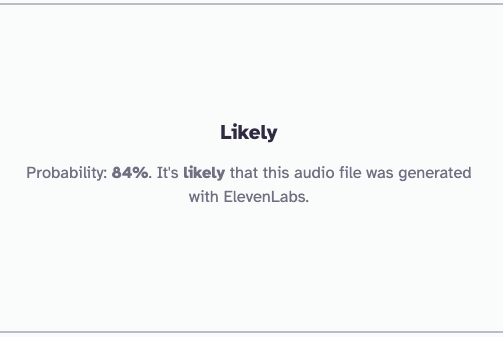
\includegraphics[width=\textwidth]{./graphics/images/sievers-11labs.png}
    \caption{Elevenlabs audio analysis \cite{elevenlabsAISpeechClassifier}}
    \label{fig:sievers-11labs}
  \end{subfigure}
  \caption{Christian Sievers DeepFake and Elevenlabs audio analysis}
\end{figure}

In the end of November 2023 \textit{two} Videos of German chancellor Olaf Scholz were released, where his voice and lips were faked. One was part of a commercial campaign for a german yellow press newspaper \cite{dwdl.deSpringerTrommeltMit}. The second is part of an art/protest project \cite{zdfKunstinstallationDeepfakeScholzVerkuendet}. Example images for these cases are not included, as they don't make any sense without the audio. It is logical, to expect a further increasing frequency of such content, both in the case of legitimate and illegitimate content.
An environment where both categories of content coexist is very challenging in regards of trust. For legitimate news makers the questions arises how it can combat disinformation and at the same time use the advancements of \gls{genai} to improve production workflows. This is a dilemma that is yet to be solved. \\
The effects of these very recent technical capabilities have not yet been studied, which is why this work attempts in doing so. In a time where the very existence of \gls{genai} raises trust issues on every kind of content, specifically of those synthetically generated, any findings about synthetic media reception might be helpful in better addressing all the named issues.

% Third Paragraph
% CORE MESSAGE OF THIS PARAGRAPH:
%\todo{P3.1. What have you done?}
This paper tried to explore the effect on potential recipients of (partially) synthetically created or AI enhanced media in the specific context of a german \gls{psm} news show. To be more specific, the focus of the research questions were: 

\todo{Forschungsfragen final fixen}
\begin{enumerate}
  \item Trust and credibility in media with varying the degree of artificiality.
  \item Effects of a "generated with AI" watermark on the material.
  \item Correlation with participants' media and AI literacy
  \item Correlation with the used screen size.
  \item Finding the most significant of the aforementioned variables.
\end{enumerate}

\todo{fix duration of study and numbers}
The questions were answered with the help of an online survey. It has been conducted within 31 days from the 6\textsuperscript{th} of November 2023 until the 6\textsuperscript{th} of December 2023. During this timeframe 159 participants answered the questionnaire. The details and results will be described within section \ref{chap:study}. \\
Before conducting such a study, the content itself needed to be created to ensure a high degree of controlability of certain variables. To accomplish this, several workflows had to be established which included several experiments with various \gls{oss} tools and chaining them together. In addition to the AI software, tradition video editing tools like \gls{prpro} and \gls{ae} came into play. The specific creation of the material is described in section \ref{implementation}. The author conducted the work in association of the german public broadcaster \gls{br} and the \gls{hff} and had an employment relationship with \gls{br} as a working student.

%\todo{P3.2. What is new about your work?}
The Methodology seeked to conduct a study about trustworthiness on various AI generated or assisted videos.
The tested videos were carefully designed by taking into account an extensive toolchain of available open source technology, making it (theoretically) possible for every media producer to recreate similar results implement (semi)automatic workflows for their media production and conduct further experiments. However the specific code implementation won't be directly shared as the risk of misuse of this project should be reduced. \\
As the tools are very recent developments, to our knowsledge, no comparable studies have been conducted yet.

% Fourth paragraph
% CORE MESSAGE OF THIS PARAGRAPH:
\todo{P4.1. What did you find out? What are the concrete results?}
\todo{P4.2. What are the implications? What does this mean for the bigger picture?}

\chapter{Background}
\label{chap:background}

This work focusses on the social aspects of synthetic media consumption, therefore related work is less technical as will be visible in section \ref{chap:rel-work}. However for the study and accompanying videos a lot of AI technologies have been implemented. To aid the overall understanding of the whole paper some technological background will be layed in this section.

\begin{quotation}
"Although it is difficult to pinpoint, the roots of AI can probably be traced back to the 1940s, specifically 1942, when the American Science Fiction writer Isaac Asimov published his short story \textit{Runaround}" \cite*{haenleinBriefHistoryArtificial2019}. 
\end{quotation}

On the other side of the imaginary, the pracitcal science was evolving during wartime. After Alan Turing famously engineered a computer to crack the Enigma cryptography he published his seminar article "Computer Machinery and Intelligence" where he described how to create intelligent machines and in particular how to test their intelligence \cite{haenleinBriefHistoryArtificial2019}. 
In the following years the term "artificial intelligence" rose to more prominence, most notably at Dartmouth College, where Marvin Minsky and John McCarthy hostet the \textit{Dartmouth Summer Research Project on Artificial Intelligence (DSRPAI)} in 1956 \cite{flasinskiHistoryArtificialIntelligence2016}. \\
The different times of where AI had its highs and lows are often refered to as the Fours Seasons of AI. Spring, representing the dawn of AI was followed by the Summer: After the events at Dartmouth college, a lot of funding by US Institutions suchs as DARPA or the RAND coorporation went into AI reasearch. Without going to much into the details of various developments, one can state that this first hype abruptly ended around 1973 where the high governmental spendings where cut. The first AI winter is often credited to Marvin Minsky and Seymour Papert, who published their famous book “Perceptrons” \cite{minskyPerceptronsIntroductionComputational2017} in 1969, in which they showed the strong limitations of perceptrons, e.g., the inability to compute some logical functions like XOR. As a result, many AI researchers concluded that the study of neural networks is not promising \cite{flasinskiHistoryArtificialIntelligence2016}. \\
\Citeauthor{haenleinBriefHistoryArtificial2019} state that, although the Japanese government began to heavily fund AI research in the 1980s, to which the U.S. DARPA responded by a funding increase as well, no further advances were made in the following years. This can only be partially held true, because some progress had to be made before the second AI summer came around: Notably multi-layer Perceptrons and therefore Deep Neural Networks in 1965, Backpropagation in 1970, Convolutional Neural Networks in 1979, Autoencoders in 1986, Generative Adversarial Networks 1990, to name just a few \cite{schmidhuberAnnotatedHistoryModern2022}.

\begin{figure}[h]
  \centering
  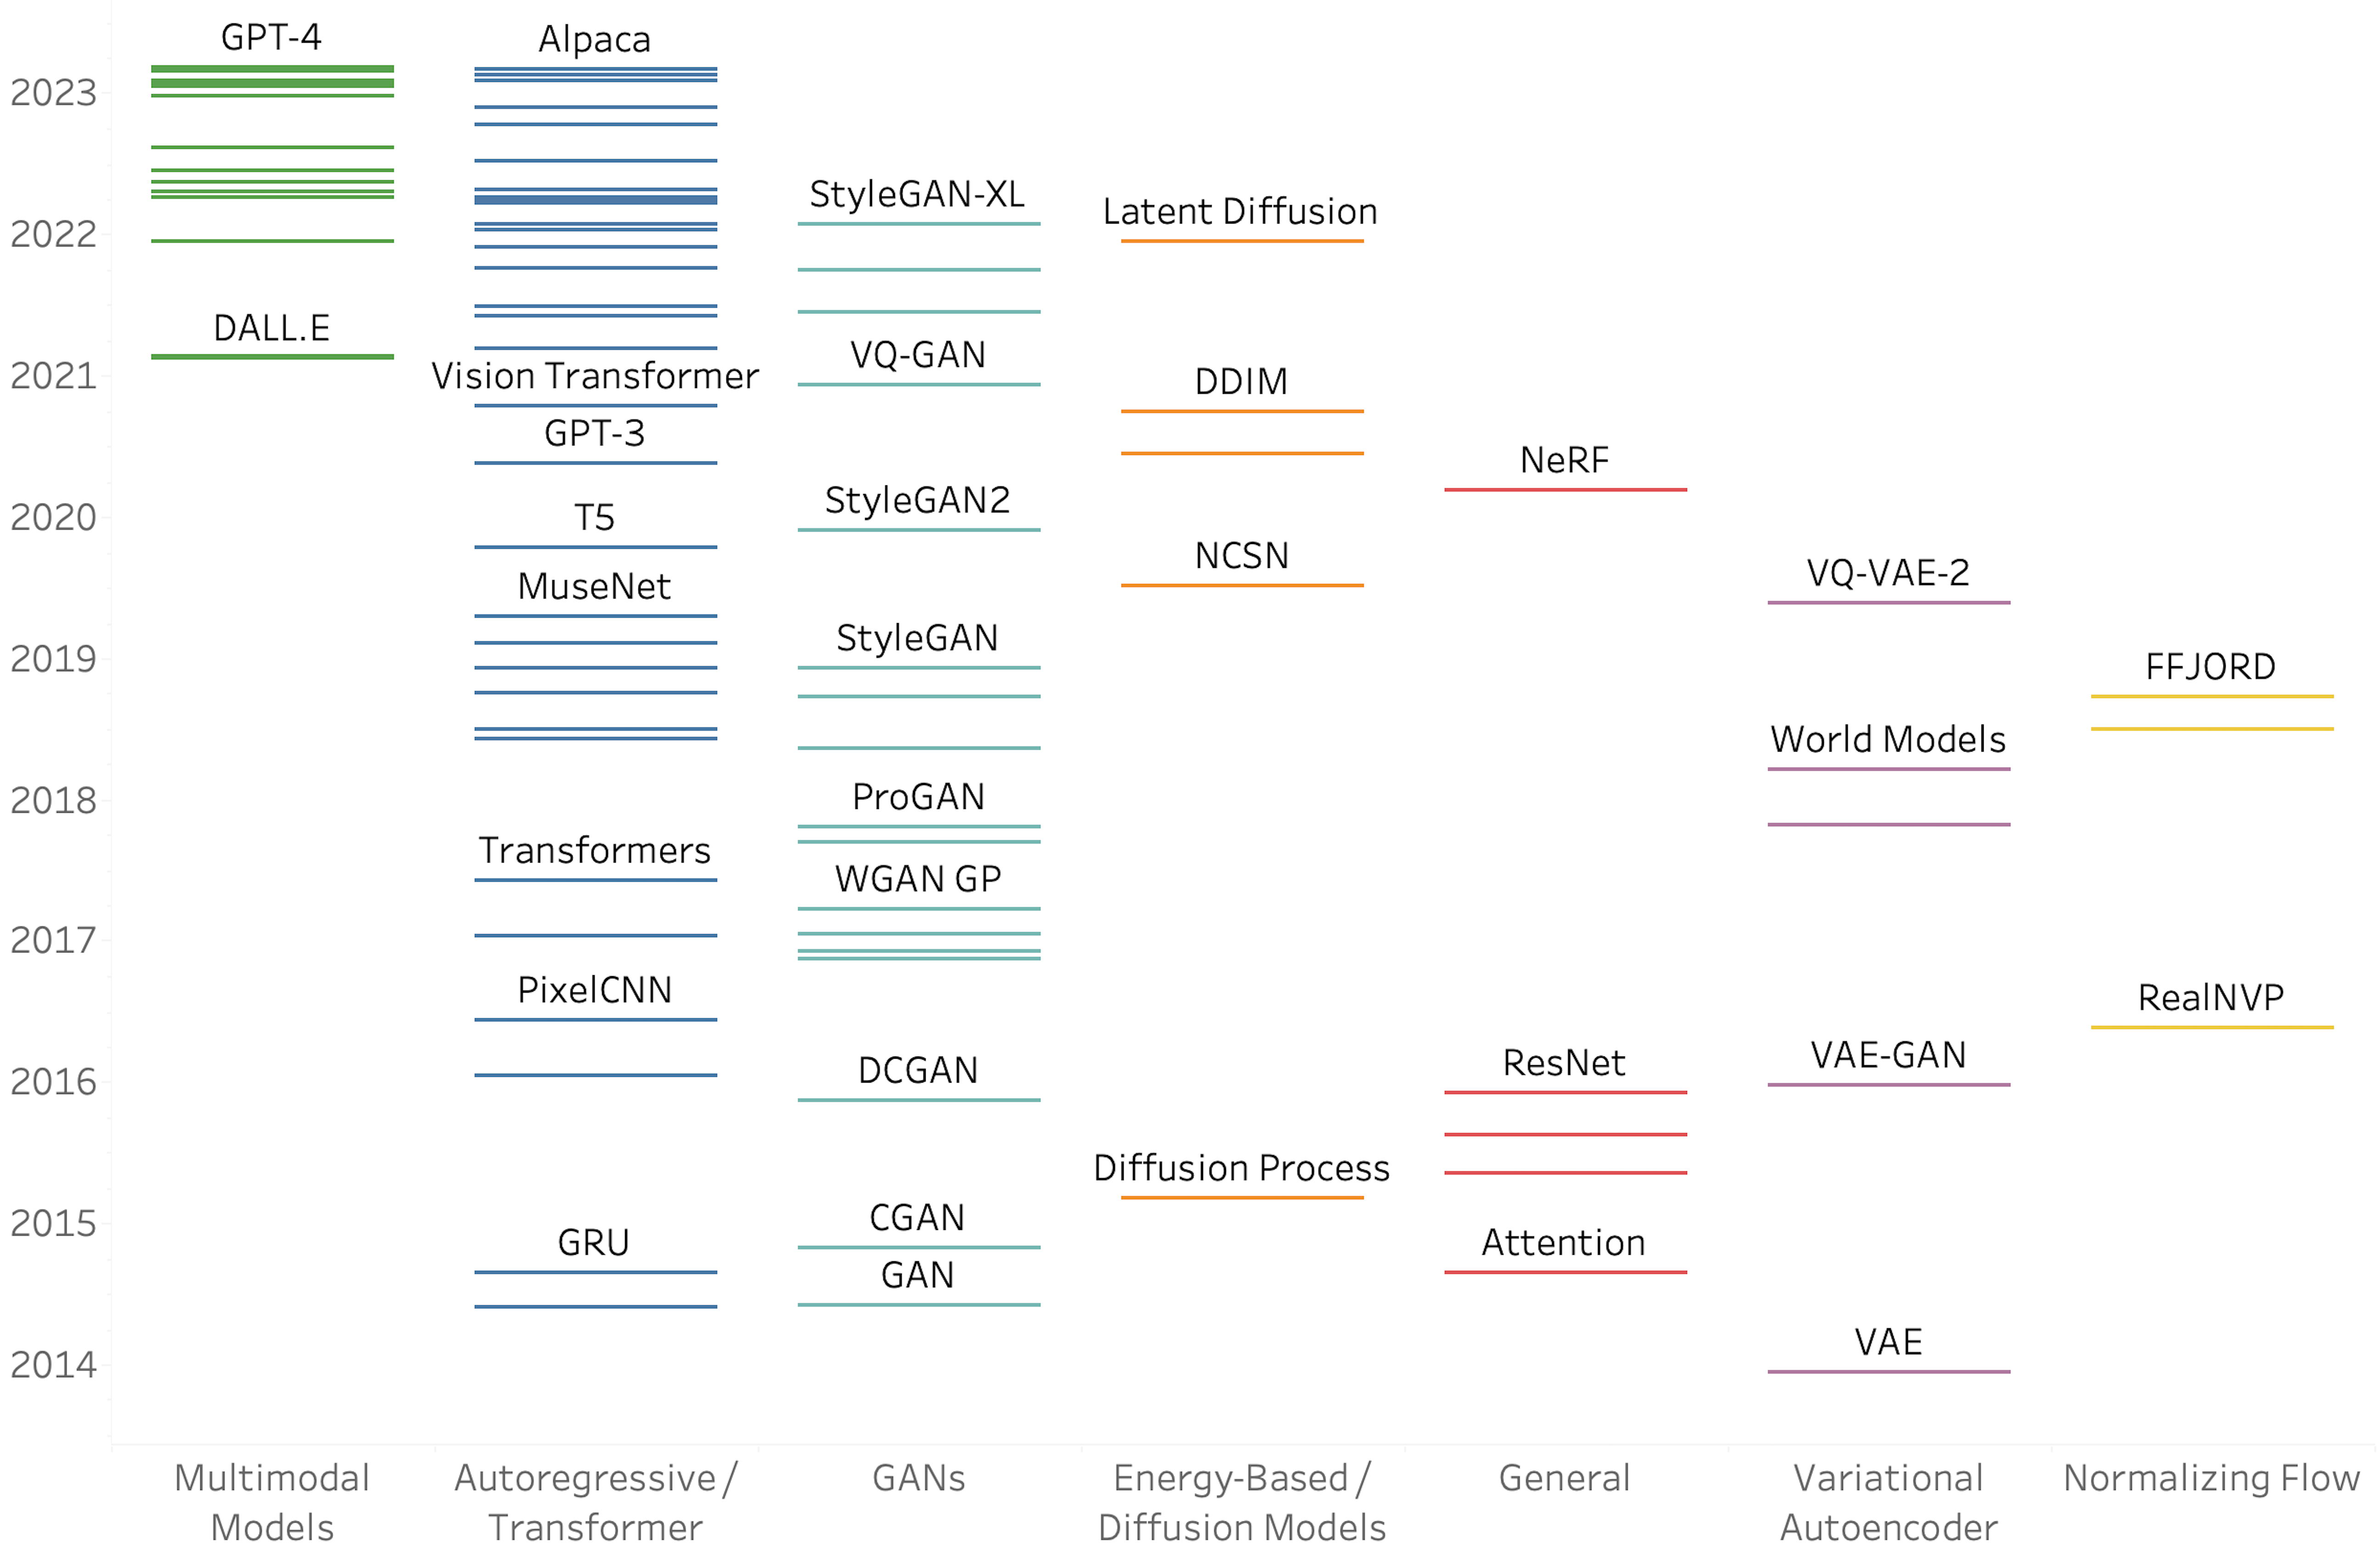
\includegraphics[width=0.9\textwidth]{./graphics/images/Timeline_of_generative_models_by_type.png}
  \caption{Timeline of generative models by type. \citet{garcia-penalvoWhatWeMean2023}}
  \label{fig:timeline-models}
\end{figure}

The AI summer arrives with \citet{krizhevskyImageNetClassificationDeep2012} and their significant advancements in image recognition using a convolutional neural network, "AlexNet". Their Network performed considerably better than the previous state-of-the-art. In 2015, AlphaGo followed with being the first AI to beat Grandmasters in the game Go. \\
Besides the image recognition domain, text and natural language processing received huge performance improvements with \citetitle{vaswaniAttentionAllYou2023} and their "Transformer" architecture in 2017. \gls{tts} also benefitted from transformer research with with major advancements in \citetitle{wangTacotronEndtoEndSpeech2017} in 2017 \cite{wangTacotronEndtoEndSpeech2017}. And to name one of the most recent advancements, diffusion based approaches are to be mentioned, which gave the powerful \gls{t2i} generator Stable diffusion its name. \cite{rombachHighResolutionImageSynthesis2022}. A chronological overview of the model developments can be depicted in figure \ref{fig:timeline-models}. \\
As the scientific advancements are numerous, so are their practical implementations. Those relevant to this work will be shortly described below.

\section{Generative AI}
\label{sec:genai}
The term \gls{genai} has been briefly mentioned in the introduction, but for better understanding the term shall be examined deeper to avoid misunderstanding in ambiguity. There is no globally agreed definition for "Generative AI" \cite{garcia-penalvoWhatWeMean2023}.

\begin{figure}[h]
  \centering
  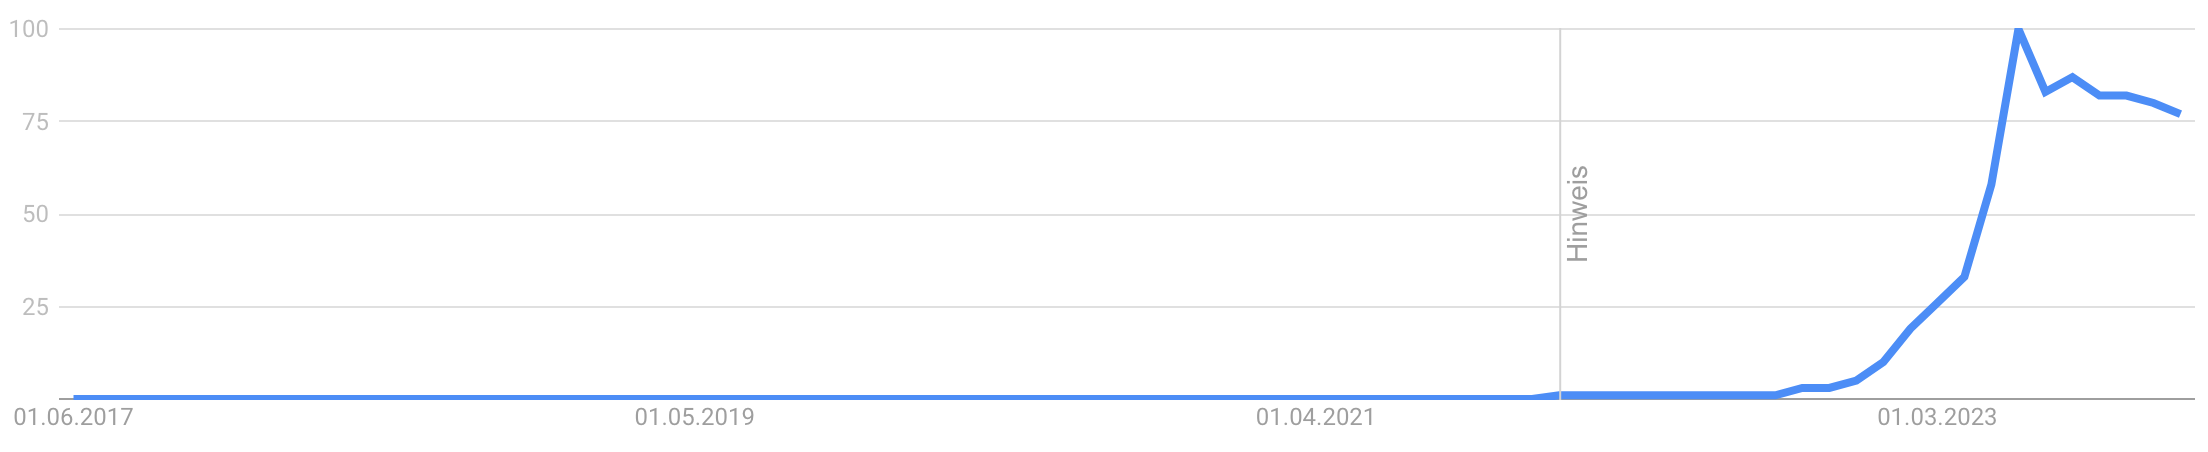
\includegraphics[width=0.9\textwidth]{./graphics/images/gtrends_genAI_1712-2312.png}
  \caption{Google Trends of "generative AI" from December 2017 to December 2023 \cite{googletrendsGoogleTrendsQuery}}
  \label{fig:gtrend-genai}
\end{figure}
\begin{figure}[h]
  \centering
  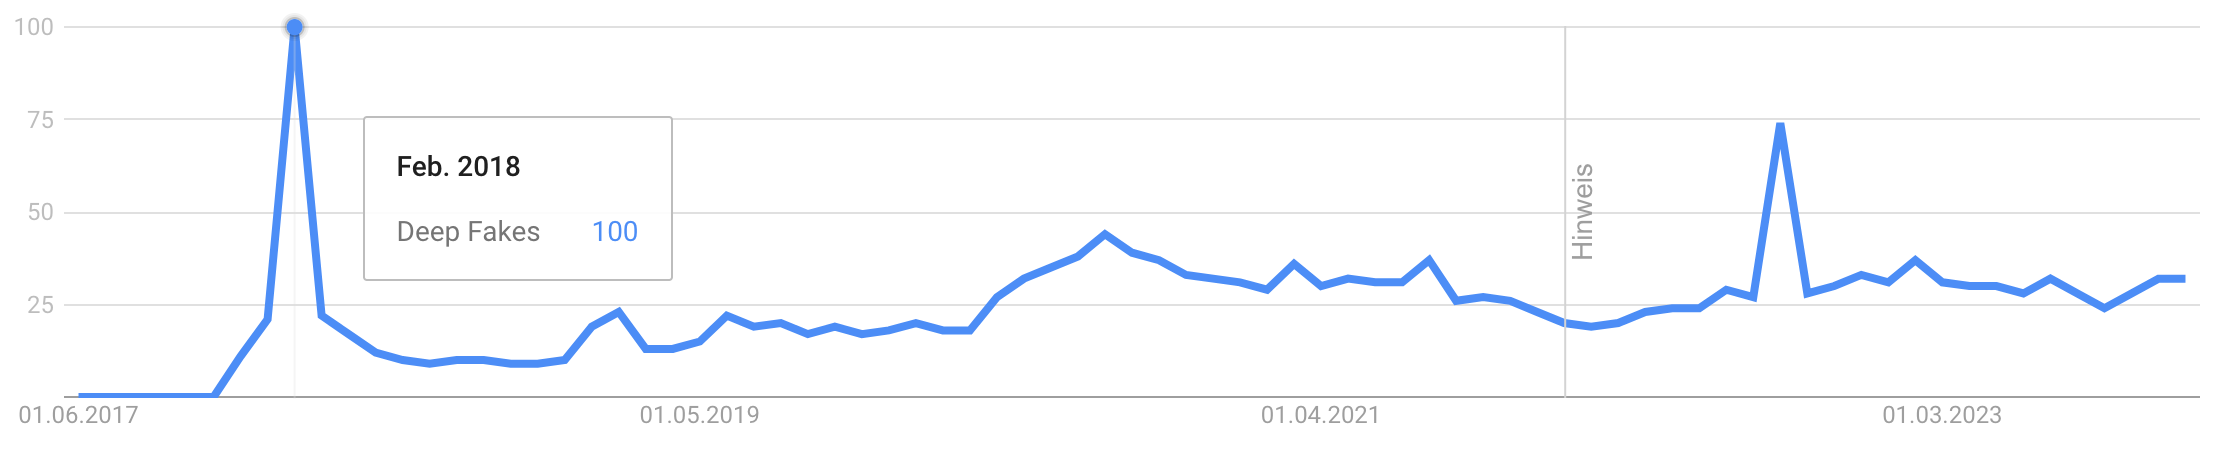
\includegraphics[width=0.9\textwidth]{./graphics/images/gtrends_deepfake_1712-2312.png}
  \caption{Google Trends of "Deep Fakes" from December 2017 to December 2023 \cite{googletrendsGoogleTrendsQuerya}}
  \label{fig:gtrend-deepfakes}
\end{figure}

For the scientific community a generative model, as described with a \gls{gan}, refers to a specific subform of neural networc architecture. These are differentiated from discriminative models by their internal processes and the probabilities they estimate \cite{garcia-penalvoWhatWeMean2023} in \cite{gmComprehensiveSurveyAnalysis2020}. \\
It is unlikely, that the broader public refers to the same, deeply technological context. It is more likely that the meaning is less about technical implementations, but more of how and end user utilizes the software: If things can be generated using AI it is generative AI. This notion can be supported by google trends of "generative AI" as depicted in figure \ref{fig:gtrend-genai}. The search requests begin to rise in October of 2023 and then climb high from December 2023 onwards. This fits perfectly to the release of ChatGPT and the spread of image generation software and their media coverage. \\
In the following the term "\gls{genai}" will be used in the means of the broader public and not the narrow technical definition. If technical details are to be discussed, they will be elaborated further. 

\section{Uncanny Valley}
Besides the technical terms we have to quickly cover the uncanny valley as well. The concept of the uncanny valley was first described by Masahiro Mori, robotic professor at the Tokyo Institure of Technology. He hypothesized that a person's response to a humanlike robot would abruptly shift from empathy to revulsion as it approached, but failed to attain, a lifelike appearance \cite{moriUncannyValleyField2012}. Some example on this spectrum are given in figure \ref{fig:uncanny-valley}.
\begin{figure}[h]
  \centering
  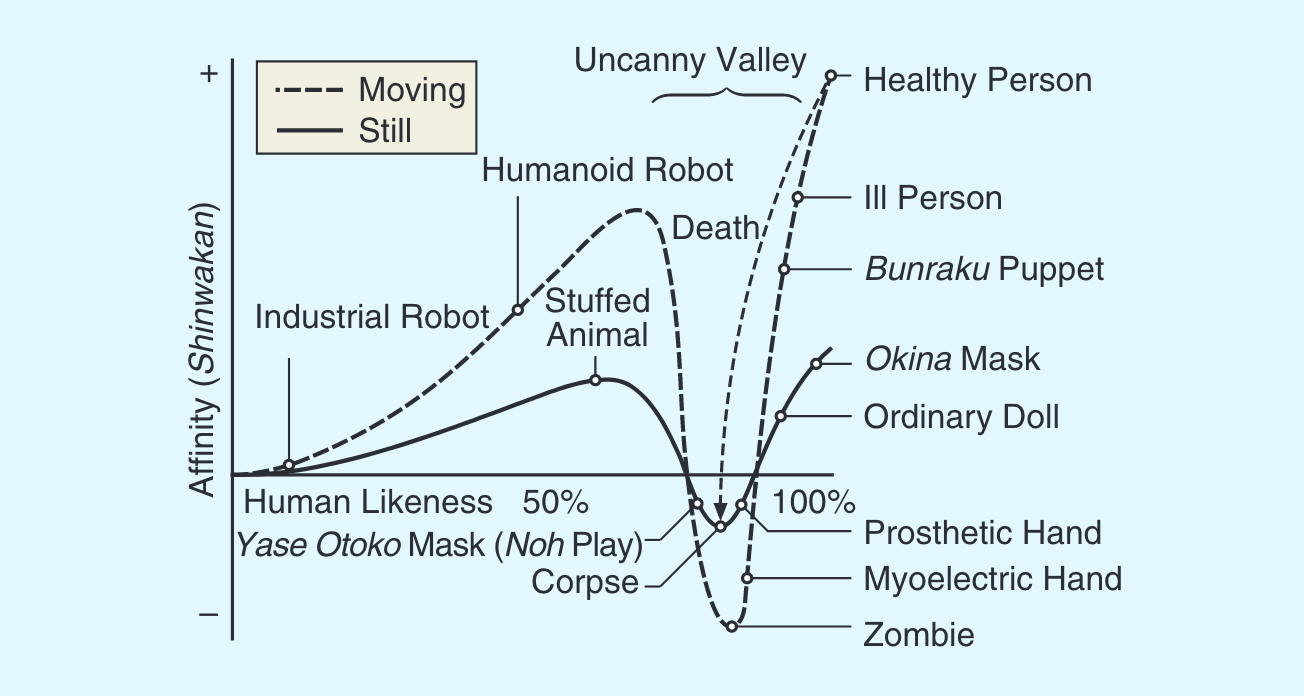
\includegraphics[width=0.9\textwidth]{./graphics/images/uncanny-valley.png}
  \caption{Uncanny valley according to Masahiro Mori \cite{moriUncannyValleyField2012}}
  \label{fig:uncanny-valley}
\end{figure}
We've needed some knowledge of the uncanny valley, because we had to take its effect into account for each test case within our study. As we investigate the trust towards AI aided news we have to consider that loss in trust could also be related with uncanny valley effects. \\
Section \ref{sec:rel-studypart} will cover the works of \citeauthor{weismanFaceUncannyEffects2021} who investigated the trust loss due to the uncanny valley in a study. \\
We will address how we handled the effect of the uncanny valley in our study design in section \ref{subsec:study design}
.

\section{ChatGPT}
ChatGPT has been used at several points to conduct this research. Especially during the software development phase(section \ref{implementation}) and the study design (section \ref{chap:study}) ChatGPT has been consulted to speed up the processes massively. \\ 
For study's content generation it did not play any role and thus won't be discussed as deeply as the other technologies. However we must consider the mere existence of ChatGPT in the context of the time this work is being conducted. As discussed in section \ref{sec:genai} the public attention towards AI tools has been tremendosly accelerated by the broad availibility of ChatGPT. When compared to the, in comparison slow and steady, increase of the google trends about DeepFakes in figure \ref{fig:gtrend-deepfakes} we can clearly see a more disruptive tendency on the timeline of ChatGPT.
The fact of how public education could influence the study shall be addressed in the study design by questioning the AI literacy among all participants. 

\section{Face Swapping}
\label{sec:face-swapping}
Similar to the previous section about ChatGPT, FaceSwaps have not been used directly within this project to create media but have played very important rule in shaping public opinion about synthetic media. As mentioned in the Introduction these FaceSwaps initially gave synthetic media the name \textit{Deep Fake} that is being used today. This fact often shifts synthetic media to have a negative connotation. \\
Besides an alerting problem with deepfake pornography and revenge porn, the first publicly recognized DeepFakes were those of Obama(Jordan Peele)\cite{vincentWatchJordanPeele2018} in 2018. \citet{hancockSocialImpactDeepfakes2021} state, that the Obama video is likely the most canonical, if not the original "deepfake" video.
Comparing it with figure \ref{fig:gtrend-deepfakes} this also fits into the timeline with the google trend search. These early DeepFakes are also responsible for the few research papers being conducted on that topic. They will be featured in chapter \ref{chap:rel-work} about the related work. Therefore this section will focus only on the technical side of FaceSwaps. \\
Prior to this paper, extensive experiments have been conducted with different FaceSwap toolkits. In the end, no FaceSwaps have been performed for the study examples. The reason for this decision lies in the study design: Briefly captured, a controlled environment was needed in order to rule out as many disruptive factors as possible. The TV-News setup was chosen as it provided a steady setting. In this case FaceSwaps were not needed. They could have been optionally used to improve the final quality of the rendered faces, but due to time constraints, this approach was not carried out. The idea will be picked up again in section \ref{sec:lips} when the quality of lip remapping is addressed.
Still, the findings about FaceSwaps are interesting as Background context of this work and thus will be included shortly in the following paragraphs.

\subsection{DeepFaceLab}
\begin{figure}[h]
  \centering
  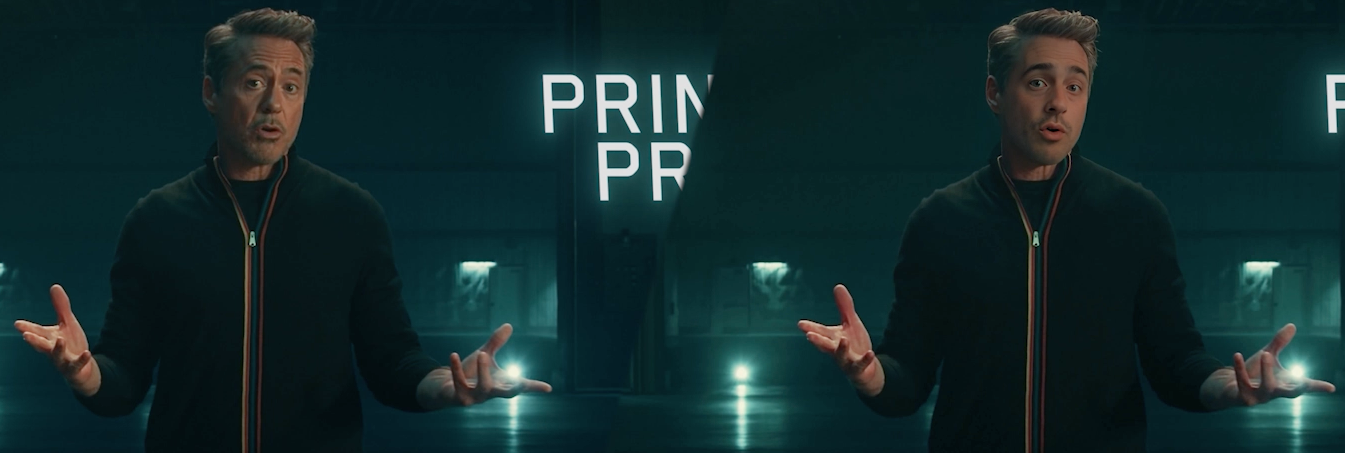
\includegraphics[width=0.9\textwidth]{./graphics/images/dfl-demo.png}
  \caption{DeepFaceLab Test result from September 2021}
  \label{fig:dfl-sample}
\end{figure}
By far the leading Software for face swapping is DeepFaceLab or DFL for short. It is also one of the first and oldest in the growing row of synthetic media creation tools. It encompasses a broad workflow in order to create high end face models. According to the commit history \gls{dfl} came into existance in June 2018 \cite{iperovCommitsIperovDeepFaceLab}. Without being able to say it with certainty, DFL's success might also lie in its proximinty to pornography. The reason for this suspection is that the main guide for how to work with \gls{dfl} is hosted as a subpage of \textit{mrdeepfakes.com}, which claims to the largest DeepFake porn site. To our knowledge these topics were rarely addressed by the authors of the software. As of November 2023 the software has been phased out of development into archive by the lead developer without providing any reasons. Probably this has to with the upcoming of newer, faster methods of face swapping discussed in section \ref{sec:roop}. For the high end workflow \gls{dfl} can still be used and there are other alternatives. \textit{FaceSwap}, actually being the first tool introduced in 2017, is under development. The standard workflow for creating a DFL model is as follows. \\ 
The terms \textit{target} and \textit{source} and to be understood in that way, that the target is the face that will be driving the final face. The source is the face that is being faked onto to target.
\textbf{Data gathering} involves finding the right material to train the models with. High resolution images of both, the target and the source are required but can be easily found online in videos. The final face resolution usually ranges from 128x128 up to 512x512 pixels. So the videos used for datagathering should be of such quality that the required face size can be extracted from the gathered videos. It is very important that the images cover a wide variety of facial angles, expressions and lighting situations. Usually around 8.000 face images are enough for a good fake.
During \textbf{extraction} faces of the wanted size get detected in video frames and extracted. Also facial alignment data gets embedded into the images as metadata as it is needed for the training process.
Afterwards \textbf{sorting and data refinement} is needed to ensure that face alignments have been correcly identified. This step also involves sorting out unwanted images. Exclusion criteria is blurriness or wrongly detected faces for example. Next, \textbf{mask segmentation} comes into play. Here the face gets masked out by a tool. This involves drawing manual face masks to fit the targets and sources face geometry needed for easier merging later on. In ths step obstructions in front of the face can be masked so that the model learns to mask these out as well during merging. After pre-processing is mostly finished and the \textbf{training} can begin. Training can take, depending on hardware, resolution and dataset size some days up to weeks or months to conclude. The training itself is departed into several stages where different hyperparameters have to be adjusted. After training, the final target can be \textbf{merged} with the synthetically generated face. One example of the generated quality can be seen in figure \ref{fig:dfl-sample}.
\begin{figure}[h]
  \centering
  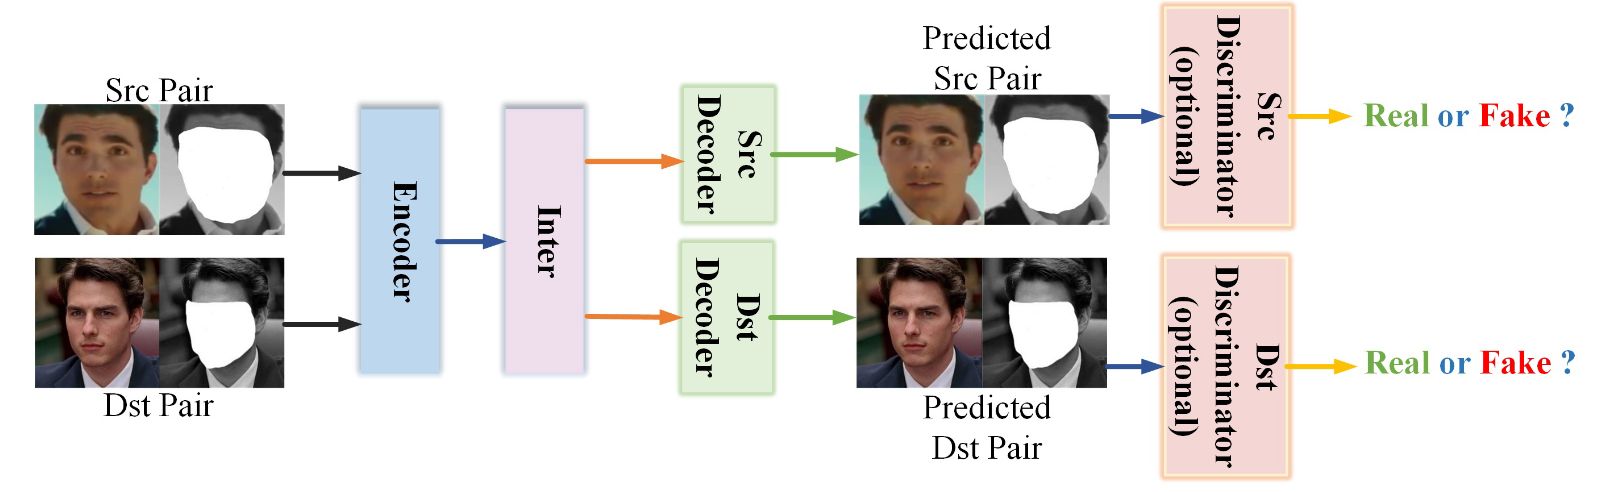
\includegraphics[width=0.9\textwidth]{./graphics/images/df-model-arch.png}
  \caption{"DF" Model architecture diagram \cite{perovDeepFaceLabIntegratedFlexible2021}}
  \label{fig:df-model-diagram}
\end{figure}

\gls{dfl} faceswaps are based on an autoencoder architecture like depcited in figure \ref{fig:df-model-diagram} though in the meantime several subvariants have developed. Autoencoders are notoriously known for their inability to create sharp images. Because of that face upscaling GAN is added within the training process. \\
As can be seen \gls{dfl} is quite complex and time consuming. On the other side it provides a great degree of freedom compared to newer methods.

\subsection{Inswapper}
\label{sec:roop}
Developed on the foundations of the InsightFace Face Analysis Project \cite{insightfaceInsightFaceWebsite} \textit{Inswapper} provides a very easy way to swap faces without the need of any training before inference. The workflow is as simple as loading a target video into the GUI of \textit{roop} \cite{sangwanRoop2023} as well as a source image and wait for the software to create the final video. The used model in the background is closed source and thus cannot be retrained. Besides the enourmous acceleration of the whole process, the lack of customization is the biggest drawback in comparison to \gls{dfl}. Overall the quality of generated Inswapper faces is quite good. The quality of the generated faces drops significantly in situations where the face is ocluded or angled in profile towards the camera. Some examples are included in the appendix under chapter \ref{chap:insightface-demos}. \\
Although not stated specifically by the \gls{dfl} developers, such rapid advancements in faceswap technology might be the reason why \gls{dfl} was discontinued. 

\section{Stable Diffusion}
\label{sec:stable-diffusion-bg}
\begin{figure}[h]
  \centering
  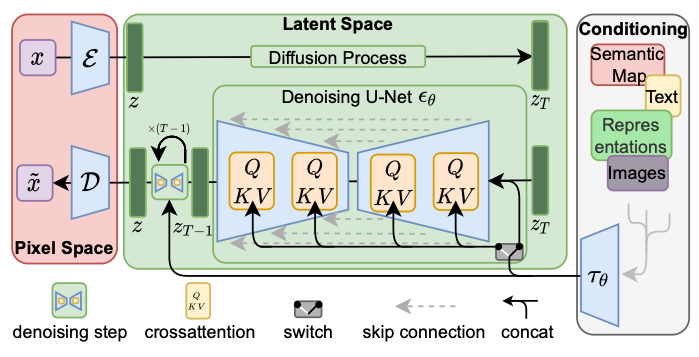
\includegraphics[width=0.9\textwidth]{./graphics/images/latent-diffusion.png}
  \caption{Latent Diffusion Model \cite{rombachHighResolutionImageSynthesis2022}}
  \label{fig:ldm-arch}
\end{figure}
\citet{rombachHighResolutionImageSynthesis2022} released their Latent Diffusion Model (figure \ref{fig:ldm-arch}) in Summer of 2022 and started huge movement for computer graphics. We won't go into further details about the inner workings of the LDM workflow but a brief overview is given in appendix \ref{app:diff-workflow}.\\
The open sourced workflow has been quickly adopted in multiple products and fuel several companies such as \textit{Midjourney, Pika-Labs, Runway, DI-D} and many more. Even more interesting than the appeareance of commercial solutions is the fact how quickly a huge Open Source community grew from the \gls{sd} project. Currently there are around a douzen different GUI projects available for \gls{sd}, some even featuring extensions within the GUI. To name the biggest, \textit{\gls{auto1}} lists \textbf{269} community extensions which massively extend the functionality in different directions, for example towards video generation. The project was initiated in August of 2022 has 22.500 forks and a 113.000 star rating which is an impressive rate of development \cite{AUTOMATIC1111StablediffusionwebuiStable}. \\
Midjourney, probably the best known commercial solution works over Discord interface and currently has around \textbf{17.3} Million registered users on their channel \cite{midjourneyJoinMidjourneyDiscord}. \\
Besides the development of image generator software there is also a thriving community for model development and finetuning so called \gls{lora} Models. These are then shared on platforms such as \textit{\gls{hf}} or prominently \textit{civitai.com}. While \gls{hf} is focussed on the developer side of models, civitai.com can also be seen as some sort of social network where user generated content in form of generated images is showcased. Civit hosts "thousands of high-quality Stable Diffusion models" as they currently state on their website \cite{CivitaiHomeOpenSource}. Especially \gls{lora}s are interesting as they are very small (several megabytes) compared to full fledged models (several gigabytes). LoRas help in finetuning the bigger models towards a specific goal. Because LoRas are so small they can be shared very easily within the community. It goes without saying that this sort of plug and play models are also well suited and used for pornographic purposes as well. Different to the earlier mention mrdeepfakes.com civitai.com features nudity filters and seeks to create a safer space for every kind of content. A public debate has already started if AI generated pornography will replace pornography and if that is an unwanted outcome. Surely the ethical concerns could fill a paper on their own and thus won't be discussed much further. However some will be mentioned as related work in chapter \ref{chap:rel-work}.\\
Latent Diffusion Models act not only as the core technology but also as a platform and the adoption speed and extensiability of both, the technology and also the community indicate a disruption is taking place here.
In context of this paper a stable diffusion workflow has been used to generate test videos in the style of a computer animation (figure \ref{fig:scheider-real-sd}). The used workflow will be featured later in section \ref{sec:sd-video}. 

\section{Lip Remapping}
\label{sec:lips}
After discarding the previously discussed whole FaceSwaps using \gls{dfl} as a meaningful tool for the study, lip remapping was chosen as one of the main visual technologies for this work. The base for many videos were real recordings from a news show. After creating a synthetic voice (refer to sections \ref{sec:tts} and \ref{sec:v2v}) the proper mouth movement needed to be recreated to make the videos somewhat convinceble. To accomplish a satisfying result, multiple tools needed to be chained together. First and foremost there is \textbf{\gls{w2l}}. Based on the research of \citet{prajwalLipSyncExpert2020} they provide a code implementation on GitHub \cite{mukhopadhyayWav2LipAccuratelyLipsyncing2023}. The code was adapted to fit the workflows for the creation of the study videos and explained in further detail in the implementation section \ref{implementation}. The \gls{w2l} project is also one of the older synthetic media tools, released in 2020.

\begin{figure}[h]
  \centering
  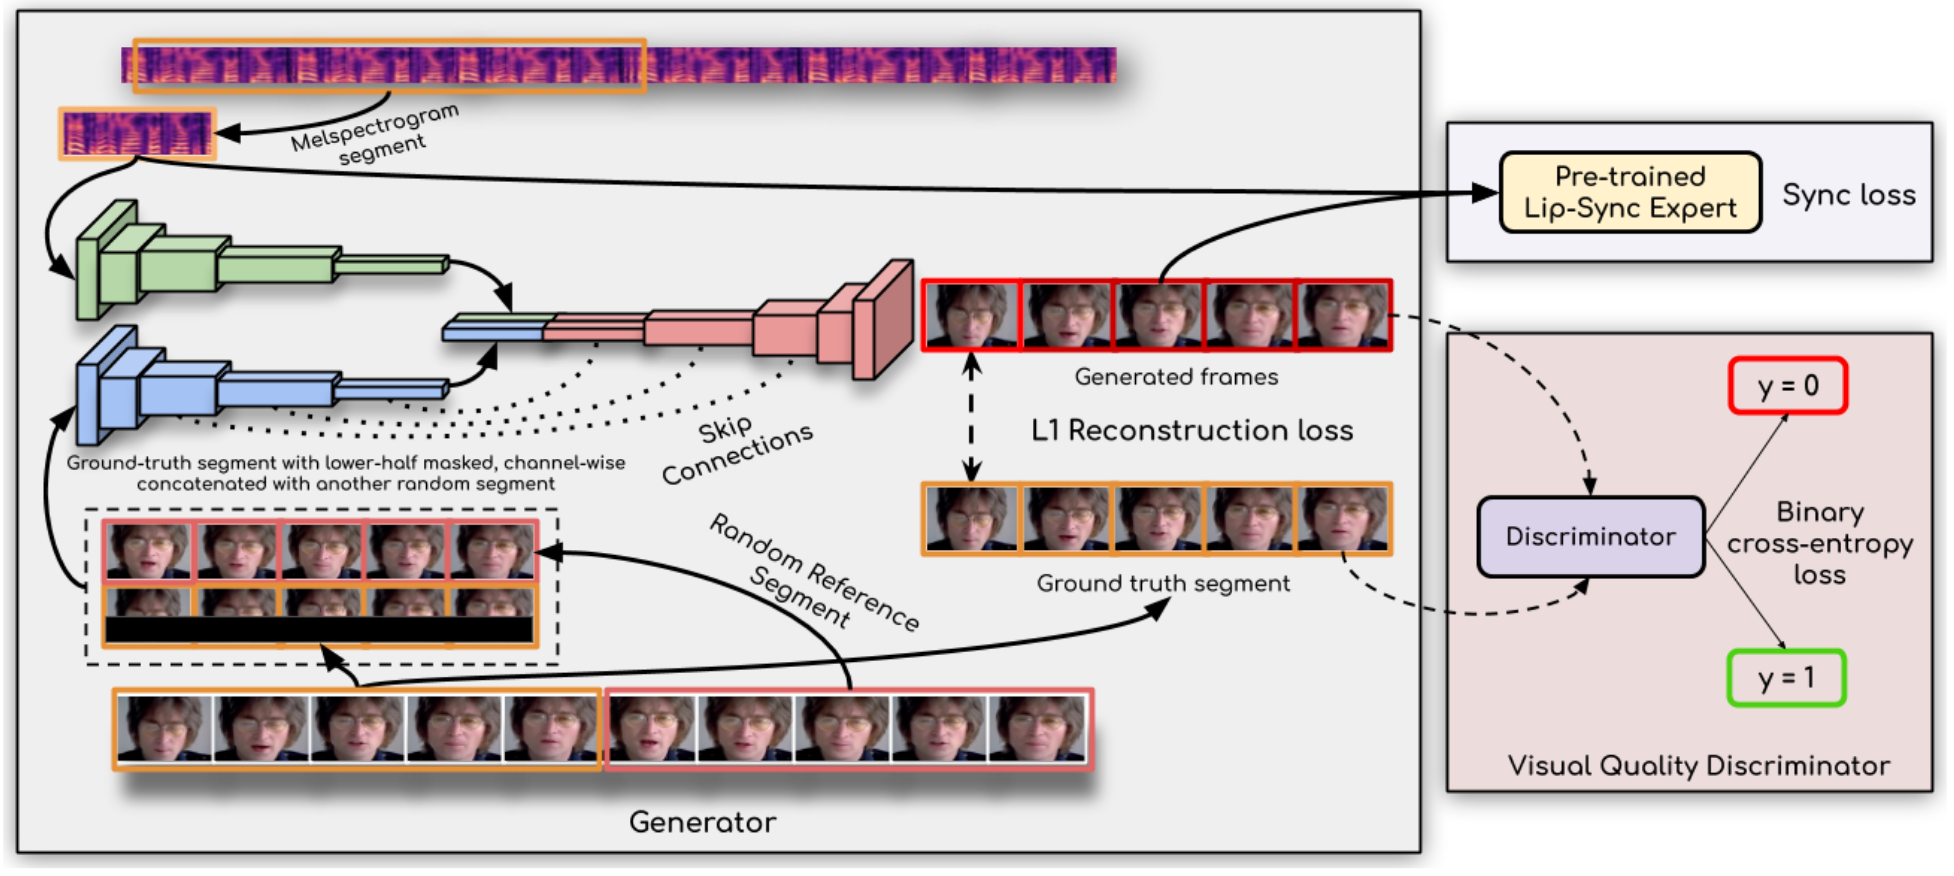
\includegraphics[width=0.9\textwidth]{./graphics/images/w2l-arch.png}
  \caption{Wav2Lip architecture}
  \label{fig:wav2lip-arch}
\end{figure}

The architecture (figure \ref{fig:wav2lip-arch}) is based on a GAN generator-discriminator approach, adding an additional "Lip-Sync Expert" discriminator which improved the results significantly in comparison to previous methods.
Unfortunately, the available public \gls{w2l} model has been trained on a face resolution of only 96x96 pixels which is insufficient for a convincing effect. To address this issue a face upsampling GAN was added to the workflow to increase the facial resolution. The upsampling was performed using the public \textbf{GFPGAN} implementation based on the works of \citet{wangNeuralSourcefilterbasedWaveform2019}. A result can be seen in figure \ref{fig:wav2lip-demo}: To the right one can see the original actor, the middle shows a \gls{w2l} result where the mouth region is blurry and the left depicts the GFPGAN upsampling. The GFPGAN workflow splits the blurry video into individual frames and upsamples each face individually. This introduces flickering artifacts in the face due to small inconsistancies after upsampling that look like flickering once played back with 25 \gls{fps}. This issue can be mitigated with further post production. \\
Overall the process of creating the lip remapping is rather slow. One 20 second video takes over 5 minutes to export. The additional post production and compositing all audio and video sources back together takes around 20 minutes after the workflow is repeated multiple times. \\
Using GFPGAN was not the only option to improve the face quality. As mentioned in section \ref{sec:face-swapping} we could have used \textbf{\gls{dfl}} on top of the \gls{w2l} output and sharpen the result with a full face swap. The method had been tested on other occasions and works quite well. It also does not have issues with face flickering. But on the counterside creating a \gls{dfl} Model is very time consuming, especially if it needs to be good. The processes within this work needed to be somewhat practical for everyday use in a media company. If every lip-remapped actor needs its own \gls{dfl} model trained this is not practical. One image swap solutions like the previously described Inswapper does not improve the quality of the \gls{w2l} outputs. \\
Ideally one would work with higher resolution \gls{w2l} or newer approaches like those from \citet{guptaGeneratingUltraHighResolution2023}. The authors state that their approach great results at 768x768 pixels compared to \gls{w2l}s 96x96 resolution. Unfortunately there was no available code implementation of the paper at the time and therefore couldn't be tested.

\begin{figure}[h]
  \centering
  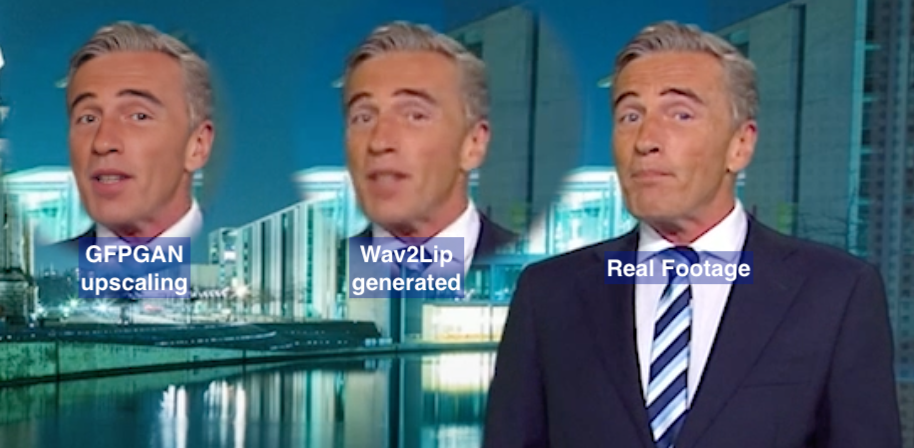
\includegraphics[width=0.9\textwidth]{./graphics/images/wav2lip/wav2lip-demo.png}
  \caption{lip remapping Workflow, described from right to left}
  \label{fig:wav2lip-demo}
\end{figure}

\section{Text to Speech}
\label{sec:tts}
To cover the audio component of the videos \gls{tts} has been used. Although there are plenty of web-based solutions (\textit{elevenlabs.io, resemble.ai}) one goal of the project was to use \gls{oss} solutions only. Regarding \gls*{tts} the decision was made to use \textbf{CoquiTTS}. CoquiTTS is a library for Text-to-Speech generation with pretrained models in +1100 languages \cite{erenCoquiTTS2021}. CoquiTTS, which developed out of a mozilla project is also community driven but also provides a \gls{saas} called Coqui-Studio. In comparison to the earlier mentioned stable diffusion community coqui's community is not as big and the community support and documentation is worse. But at least there is some documentation about training a new voice and it could be done. The results were satisfying but certainly leave plenty of room for improvement, compared the state of the art commercial solutions. \\
One of the bigger challenges in implementing \gls{tts} was the gathering and pre-processing of training data: 
In exchange with the community a dataset size of around 4 hours of speech was required to get decent results. The difficulty did not lie in getting the raw data, this was easily obtainably from the archives of the \gls{br}. In order to train the \gls{tts} model the data needed to be structured in a special format: Audio segments needed to be under 10 seconds in length and each audiofile needs accompanying transcription in a text file. To solve these issues on a scale of 4 hours of content a toolkit has been developed which will be explained in detail in section \ref{sec:dvt}.
\begin{figure}[h]
  \centering
  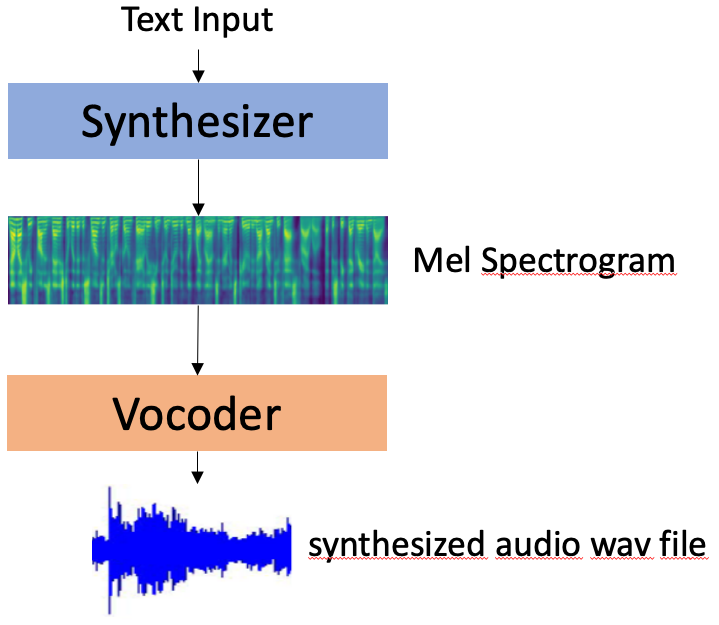
\includegraphics[width=0.75\textwidth]{./graphics/images/tts/tts-workflow.png}
  \caption{Basic \gls{tts} workflow. Image source: \cite{jemineRealTimeVoiceCloning2019}}
  \label{fig:tts-explainer}
\end{figure}
Usually \gls{tts} is accomplished by using multiple stages of training multiple models. A basic overview of how they work together can be seen in figure \ref{fig:tts-explainer}. The inputted text gets encoded as a mel spectrogram by the synthesizer. Based on these mel spectrograms the vocoder then generates an audio file. \\
Most of the architectures, implemented by CoquiTTS feature a synthesizer model, which converts the input text to a mel spectrogram and a vocoder that translates the spectrogram to an audio file. However the development in the TTS domain is rapid and many other methods have been created. 
CoquiTTS lists several implemented approaches, such as 13 spectrogram models, 5 End-to-End Models, 6 attention methods, 2 speaker encoders and 8 vocoders. These won't be covered in depth as they are not in focus of this paper. If of any interest, please refer to the CoquiTTS documentation and corresponding papers.\\
For ease of use we decided to use the VITS End-to-End model for this project developed by \citet{kimConditionalVariationalAutoencoder2021}. In contrast to the traditional multi-model approaches VITS offers full TTS capabilites by training just a single model. This approach is faster and more reliable in most cases. A downside of using VITS is fewer granular control over the models. This project favoured speed over quality and opted for the easier workflow of VITS. Naturlly the state of the art changed quickly so the current approach migh as well soon be outdated. \\
CoquiTTS also recently added a faster cloning method called X-TTS. It is also an End-to-End model like VITS but with the addition that it can be used in a zero-shot manner. This means it can reproduce voices it hasn't been trained on, which is achieved by providing a reference voice in addition to the input text. Although we do not know for sure, it probably works similar to the \gls{rtvc} toolkit by \citeauthor{jemineRealTimeVoiceCloning2019}. Most likely, Elevenlabs' "Instant Voice Clone" also works with this technology under the hood.

\begin{figure}[h]
  \centering
  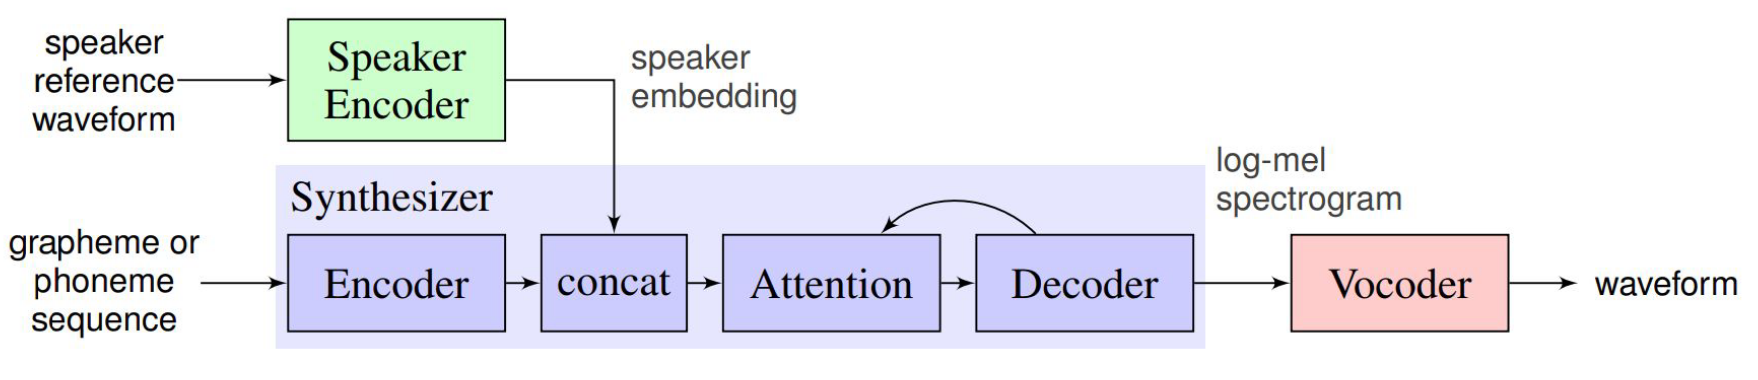
\includegraphics[width=0.8\textwidth]{./graphics/images/rtvc.png}
  \caption{RTVC Architecture \cite{jemineRealTimeVoiceCloning2019}}
  \label{fig:rtvc-arch}
\end{figure}

The \gls{rtvc} workflow clevery introduced a speaker encoder to the training process of the synthesizer (see figure \ref{fig:rtvc-arch}). The speaker encoder is based on speaker verification and voice recognition and provides a speaker embedding. The synthesizer is then trained with the speaker embeddings as an additional input. During inference one has to provide a speaker embedding (the reference voice sample). Based on the embedding, the synthesizer then produces the cloned voice without having been trained on the voice in advance. We have been experimenting with the \gls{rtvc} in 2021. At the time it only worked with english voices and we tried to create a german model as well. The results were unsatisfying. Today, with X-TTS, the german voices do not sound good enough which is why we switched back to the time consuming retraining approach with VITS. \\
Regarding our VITS training duration, we first trained a first run with 90 minutes of training material for two weeks of a RTX 4090. The second run with 4 hours of material was conducted on A6000 took approximately one week until the loss values converged. 

\section{Voice to Voice Conversion}
\label{sec:v2v}
Besides \gls{tts} another recently published approach should be tested: \gls{v2v} conversion. The main difference is that one does not input Text but actual speech into the converter and receives an audio file with the voice of the targeted voice. This approach can address the a problem with \gls{tts} where the synthesized voice sounds to monotonous. Because the tonality of the target speaker is retained after converting it to the other voice an actor can influence how the result should sound. On the counterside certain mannerisms in the actors voice will translate to the result. That can be an odd sounding pronounciation of the letter "S" or "R", hissing, or something else. \\
For accomplishing \gls{v2v} conversion the \gls{rvc} project was used \cite{RVCProjectRetrievalbasedVoiceConversionWebUI2023}. 
\begin{figure}[h]
  \centering
  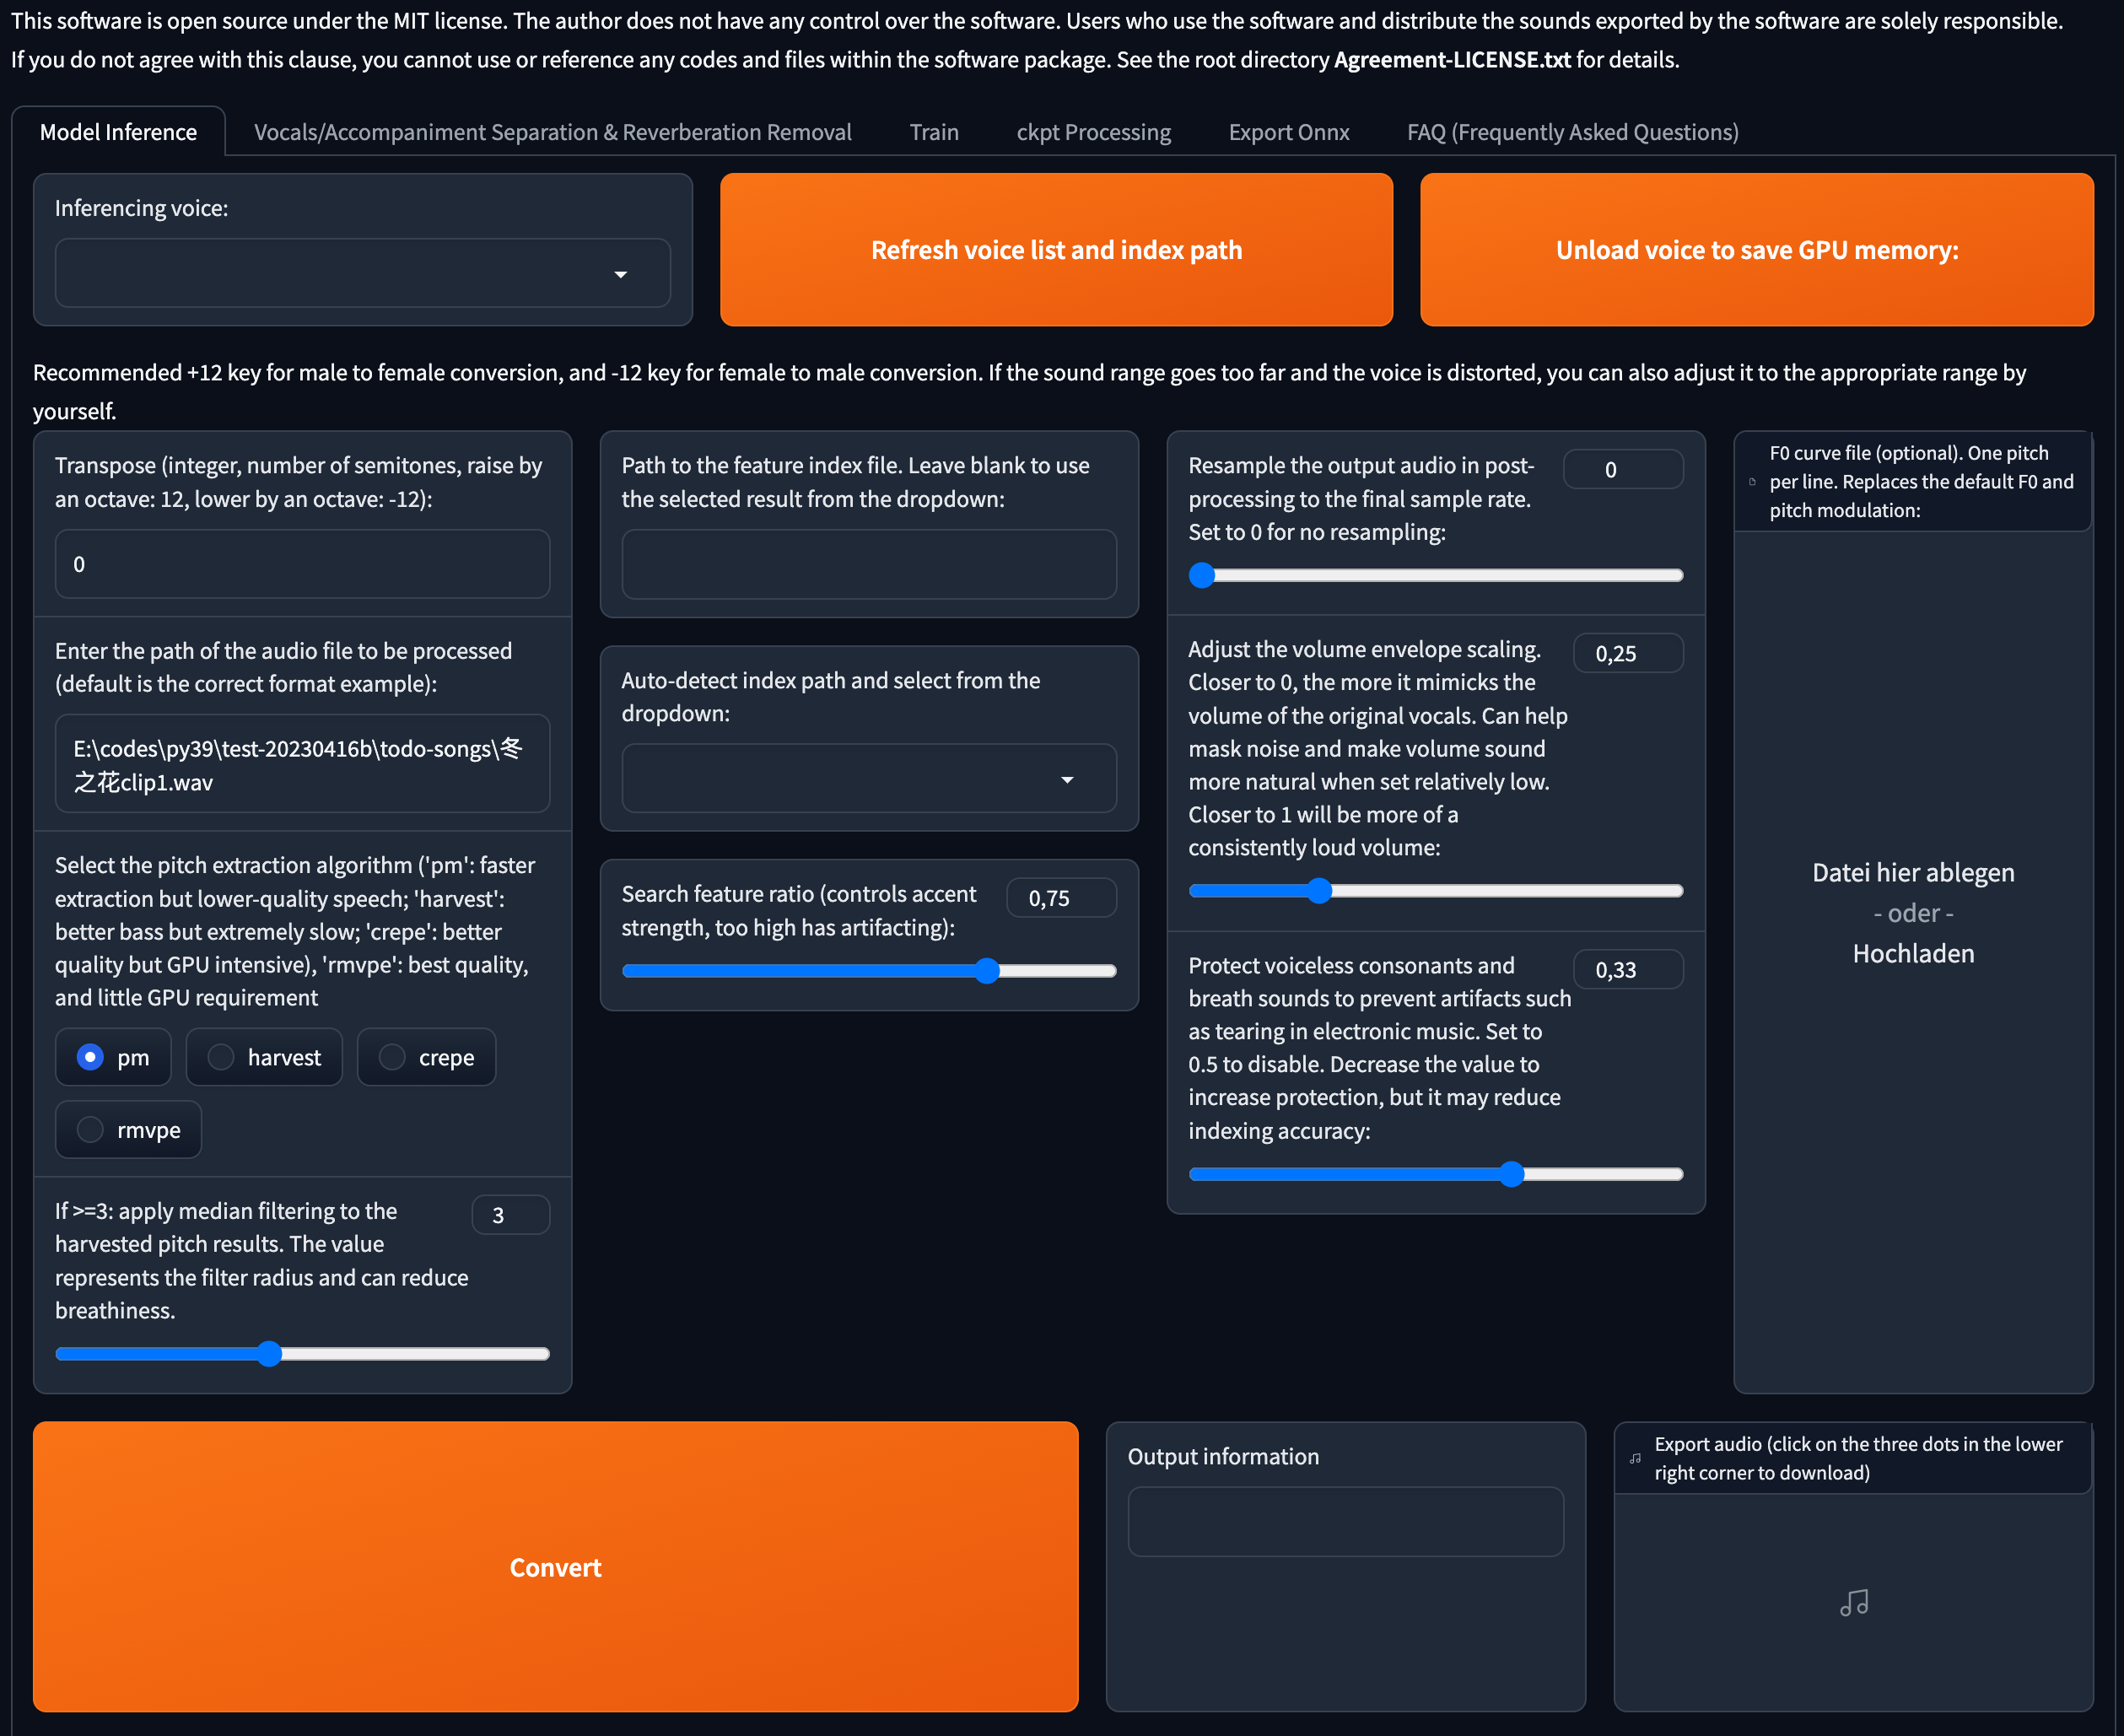
\includegraphics[width=1\textwidth]{./graphics/images/RVC-UI.png}
  \caption{RVC Gradio User Interface}
  \label{fig:rvc-gradio}
\end{figure}
The project features a gradio.io user interface (figure \ref{fig:rvc-gradio}) for easy cloud deployment and is quite self expalinatory. Regarding the dataset requirements, approximately 10 minutes of a person's voice is required. The data pre-processing does not require any textfile transcription as with \gls{tts} but does need cutting up the voice samples in sections under 10 seconds to avoid an \gls{oom}. This can be easily achieve with the pre-processing toolkit developed for the \gls{tts} section of this work. The training itself takes approximately one hour on an A6000 GPU. \\
After training is completed inferencing the model is very fast. With \gls{rvc} it processes inputted audiofiles in near realime. It is to be noted, that there is an implementation of a real time voice changer for these models \cite{WokadaVoicechangerVoice}. One can use input from a file or microphone and the voice changes with very little delay (100ms on a suitable graphics card). The implications of such realtime voice fake capabilities are very interesting in the domain of DeepFakes and scams. There have been some reports that fake voices have been used to conduct scams. However these were often accomplished using \gls{tts} and prepring the sound snippets for playback. Combining such a technology with the real time FaceSwaps calls for caution and multifactorial security in videocall-based social interaction. \\
Interstingly these voice models are shared as well among creators on platform such as civitai but the technology has not yet had such an impact to broader society as stable diffusion had. \\
\gls{v2v} models could also be used to improve \gls{tts} quality in a similar fashion as suggested with Wav2Lip and FaceSwaps: One could train a faster but lower quality \gls{tts} model and then upsample the voice quality in realtime with \gls{v2v}. No experiments were conducted in this direction due to time constraints as that would have required a shift in the \gls{tts} approach.

\section{Game Engines and virtual Production}
\label{sec:bg-virtual-production}
A few years before the big leap in \gls{genai} virtual production methods started to gain traction within the film and broadcasting industry. Instead of filming in front of a greenscreen, \textit{The Mandalorian} (2019) famously used a large LED Panel around the whole studio walls and ceiling to shoot their movie (refer to figure \ref{fig:mando-vps}). That way many effects could be achieved "in camera" opposed to "in post production" as it is done usually.

\begin{figure}[h]
  \centering
  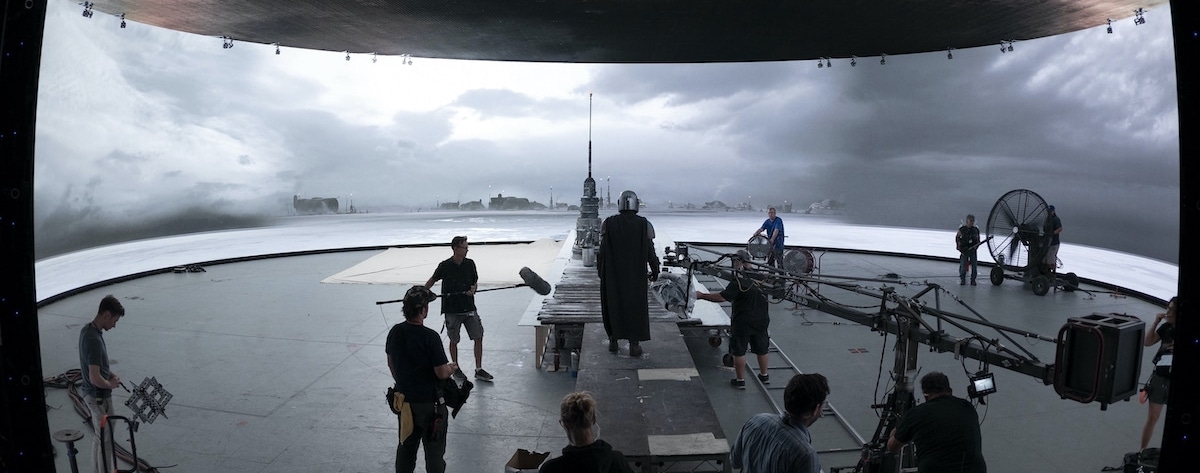
\includegraphics[width=1\textwidth]{./graphics/images/mandalorian-vp.jpg}
  \caption{\textit{The Mandalorian} Studio and LED-Volume "Stagecraft" \cite{landsiedelGamechanger2021}}
  \label{fig:mando-vps}
\end{figure}

The important shift in technology was not only the use of LED panels, but what drives the images on the screens. It is Software, usually found in the Gaming Industry: \gls{ue}, a so called \textbf{Game Engine}. The Engines capability to render photorealistic images in realtime made it the ideal driver for this novel movie production. Today \gls{ue} is can not only be used to generate environments, but humans as well. Their software \textit{Metahuman} creator allows an easy character creation. It is also possible to scan a face and transfer the geometry onto a metahuman. An example of such approach can be seen in figure \ref{fig:metahuman-comp} this process does not work perfectly well. 

\begin{figure}[h]
  \centering
  \begin{subfigure}[b]{0.45\textwidth}
    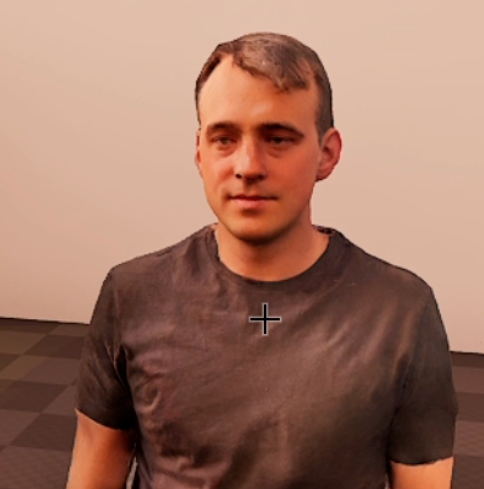
\includegraphics[width=\textwidth]{./graphics/images/photogrammetry.png}
    \caption{Photogrammetry scan}
    \label{fig:head-photogrammetry-scan}
  \end{subfigure}
  \hfill
  \begin{subfigure}[b]{0.5\textwidth}
    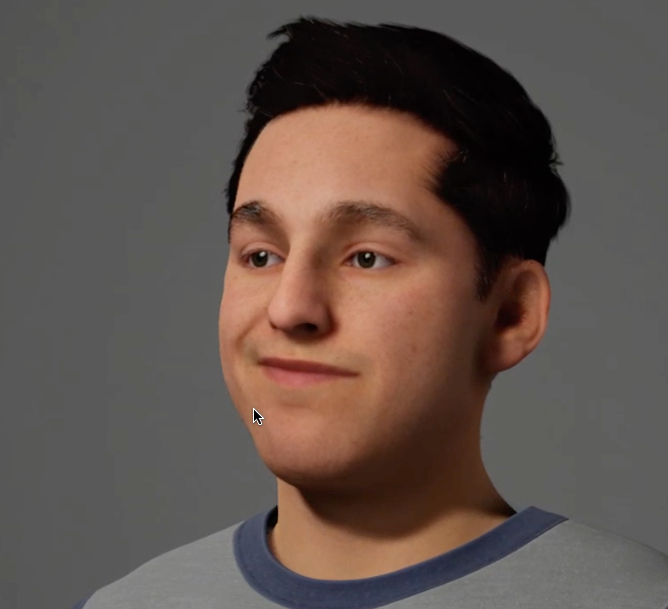
\includegraphics[width=\textwidth]{./graphics/images/Metahuman.png}
    \caption{Metahuman based on photogrammetry scan}
    \label{fig:metahuman-result}
  \end{subfigure}
  \caption{Mesh to Metahuman workflow}
  \label{fig:metahuman-comp}
\end{figure}

Already during the timeframe of creation of the videos the process for creating metahumans improved considerably. It is only a question of time until these metahumans get more advanced. Currently gaussian splatting seems to be a key technology to watch in these regards. \\
It has to be noted that \gls{ue} is a complicated tool that needs a lot of time to be mastered. In addition to \gls{ue} many other, more specialized tools need to be used to get the best possible output. These include modelling tools for environments and characters as well as texturing tools and many more. \gls{ue} in the end is good at combining all the assets, but to get high quality results a team needs expertize in many different areas of traditional computer animation. Espcially the metahuman characters fall into the uncanny valley, which makes the results unsuitable for a good study. It was explored to improve the faces quality using a \gls{dfl} model. Unfortunately the uncanny part of the face is not the appeareance of the face, but its movements. This most likely has to do with how the face is animated. The facial performance capture is being accomplished using and iPhones FaceID camera which has limitations in how many facial landmarks it can track and therefore reduces face movement fidality. Because of that the face movements do not look very natural and because the movements translate to the \gls{dfl} face as well it is of no use. \\
Even though the quality of the metahuman result was not compelling, they were included  within the study as will be elaborated in section \ref{chap:study}. 

\chapter{Related Work}
\label{chap:rel-work}
% Introduction
While Chapter \ref{chap:background} served the purpose of giving some background on the technical side and establish a general understanding of how the used technologies can be applied. Now we want to present some related work in the domain of psychological and sociological research, which has been done in the context of (synthetic) media trust and credibility and the effects of fake news in general. 

\begin{quotation}
  "[...] We urge researchers to begin to study the social issues surrounding deepfake technology. The studies in this volume do a fantastic job of mapping out the research questions, applying theory to the phenomenon, and creating new tools to apply to future research. But this study is preliminary, and we urge scholars to build upon this study as deepfake use continues to grow." \cite{hancockSocialImpactDeepfakes2021}
\end{quotation}

With this call to action, "Cyberpsychology, Behavior, and Social Networking" (volume 24, issue 3) published several articles that can be summarized as "the social impact of DeepFakes". This was in 2021, three years after DeepFake FaceSwaps have become dominant. To begin with, \citet{hancockSocialImpactDeepfakes2021} raised a few questions about DeepFakes: Does exposure to deepfakes undermine trust in the media? How might deepfakes be used during social interactions? Are there strategies for debunking or countering deepfakes? They concluded that empirical research on the social impact of DeepFakes is scarce and therefore referenced to neighbouring fields. \\
In an introduction to the topic as a whole, \citet{hancockSocialImpactDeepfakes2021} cite studies on "false memory aquisition" by \citet{garryActuallyPictureWorth2005}. These experiments often involve some doctored footage of participants, often created with tools of 3D Animation, and prove, that it is possible to induce false memories with that approach. \\
\citet{hancockSocialImpactDeepfakes2021} also mention deception research and conclude that people perform only slightly above chance when evaluating a message as either true or deceptive \cite{bondAccuracyDeceptionJudgments2006}. To quote: "Studies have shown that deception detection is approximately the same whether the message is conveyed through text (e.g., a court transcript, an Internet chat log), an audio recording (e.g., a voicemail, a radio program), or a video (e.g., an interrogation video)" \cite{hancockSeeNoEvil2010} cited in \cite{hancockSocialImpactDeepfakes2021}. \\
The references by \citet{hancockSocialImpactDeepfakes2021} show how far research in the field can reach out. In the following we will present further examples. We decided to divide the related work in three categories: In \ref{sec:hist-context} we want to provide some context about the environment in which the papers were written. In \ref{sec:rel-secondary} we shed some light on methods which don't study participants responds directly in a study, but analyze secondary indicators such as newspaper articles, forum blogposts and video comments. In \ref{sec:rel-studypart} we name controled studies, which were conducted with individual participants who consumed some kind of synthetic content. Our own paper should fall under the latter category as well. And in \ref{sec:rel-work-counteringdf} we added some works about countering maleficent synthetic media.

\section{Historical and socio-geographical Context}
\label{sec:hist-context}
As stated in the Introduction, synthetic media is a rather new trend, mainly driven by the advance of \gls{genai}. It can be dated back to earliest of 2017 when DeepFake FaceSwaps surfaced to the broader public. It is remarkable, that the term \textit{Fake News} is also a very young topic on its own and developed around the same time as DeepFake FaceSwaps around 2016. For completeness it should be noted that the \citet{merriam-websterdictionaryRealStoryFake} dates the first use of Fake news back to the year 1890. Surely skepticism has always existed towards politics and media, but it surely wasn't as a big of a topic until Donald Trump entered his presidential campaign in 2016 as can be seen in the Google trend analysis in figure \ref{fig:gtrend-fake-news} and \ref{fig:trust-us}. That said, it wouldn't make much sense to look for related work earlier than 2016/2017. Therefore we focussed our attention to the timeframe where DeepFakes came into existance and Fake News became a publicly relevant topic.
\begin{figure}[h]
  \centering
  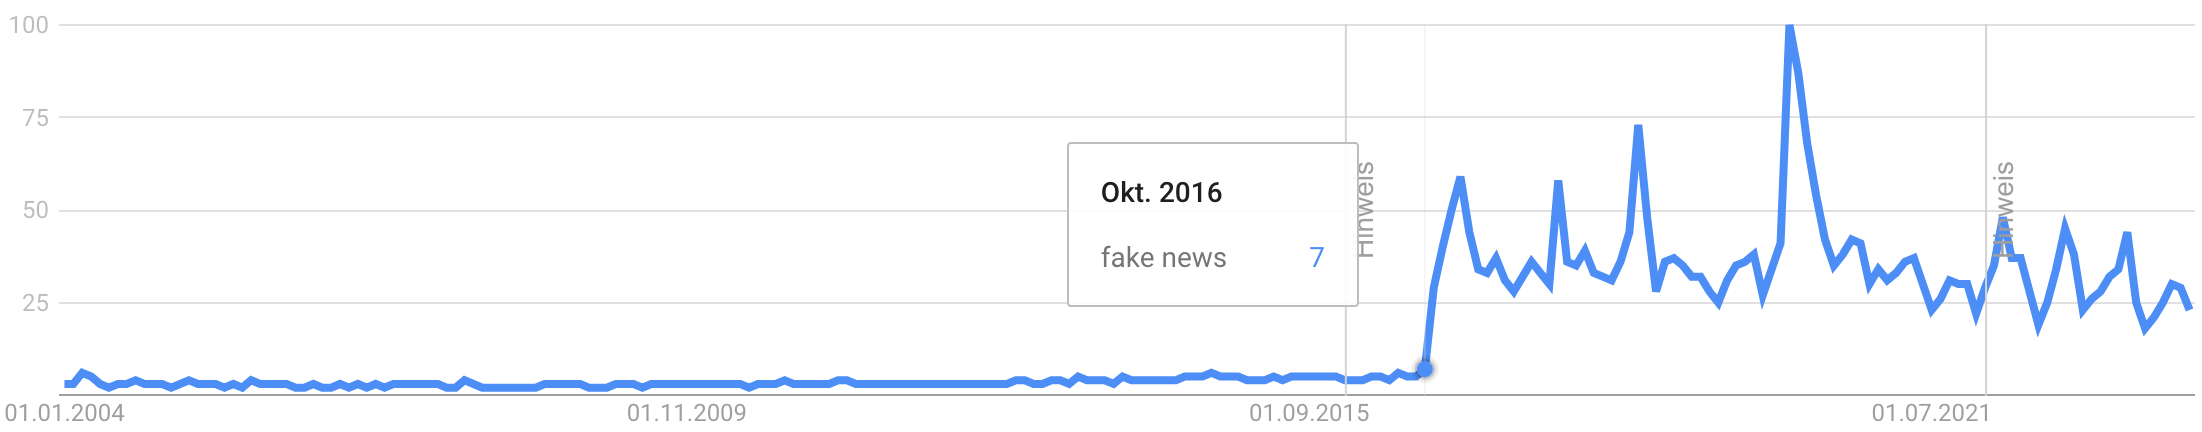
\includegraphics[width=1\textwidth]{./graphics/images/gtrends_fakenews_1011-2311.png}
  \caption{Google Trends of the term "Fake News" 2004-2023}
  \label{fig:gtrend-fake-news}
\end{figure}
In our study we investigate a german-speaking population. Therefore we want to add, that papers which are focussed on a certain terretory (mostly US in relation of Trump) can only be included with the caviat that they might not directly apply to the german cultural space as well. To illustrate one difference we can refer to figure \ref{fig:trust-ger} in comparison to \ref{fig:trust-us}. While trust among american public decreased around 2016, no impact can be seen in Germany at this time. It took until the years of the Covid19 Pandemic to experience a decline in Germany as well. It remains to be seen how this trend will continue in the following years.
\begin{figure}[h]
  \centering
  \centering
  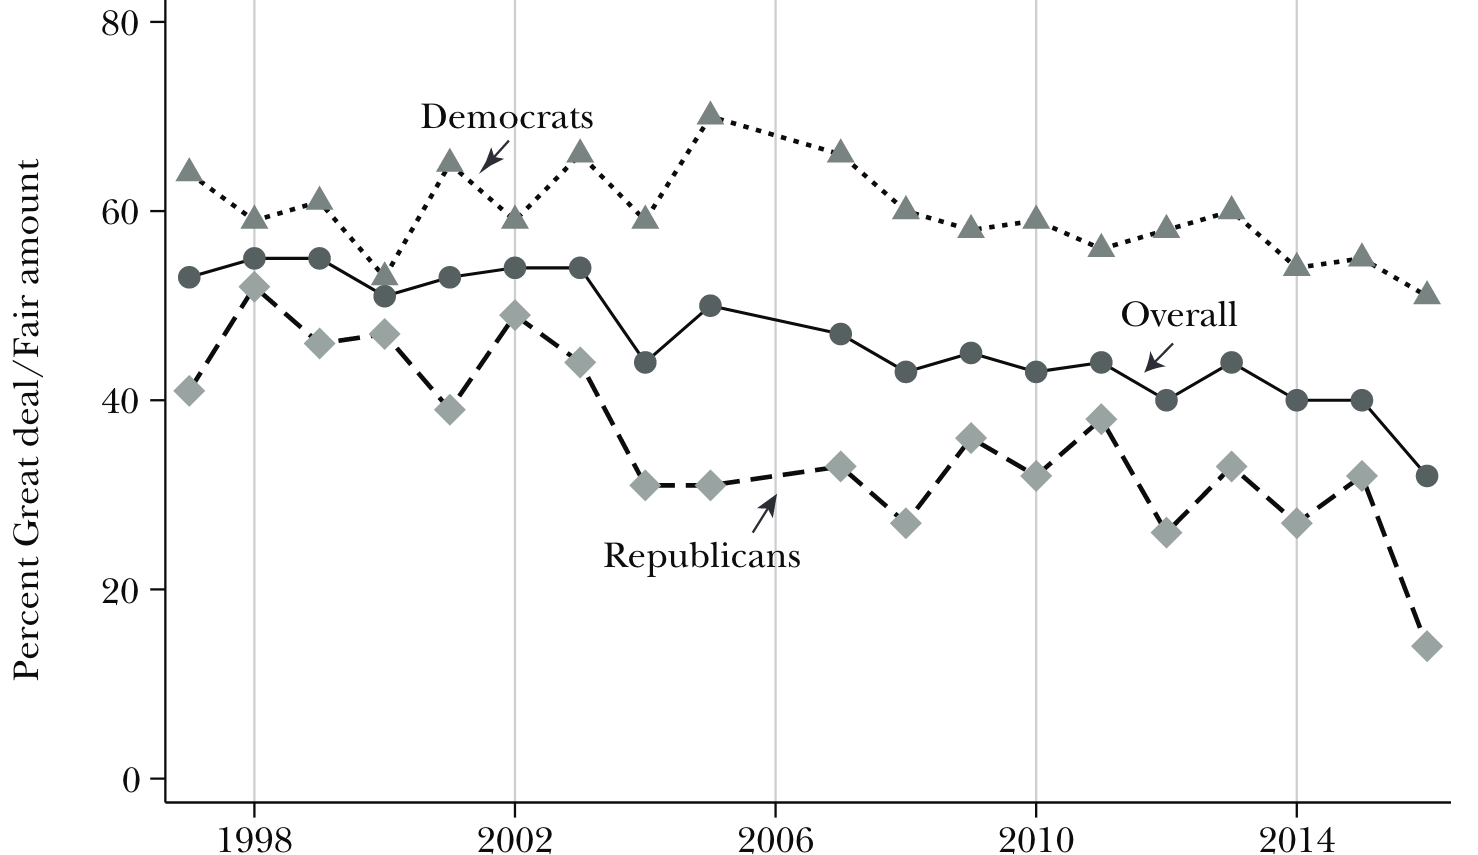
\includegraphics[width=0.75\linewidth]{./graphics/images/trust-america mainstream.png}
  \caption{Trust in American Mainstream Media 1996-2017 \cite{allcottSocialMediaFake2017}}
  \label{fig:trust-us}
\end{figure}
\begin{figure}[h]
  \centering
  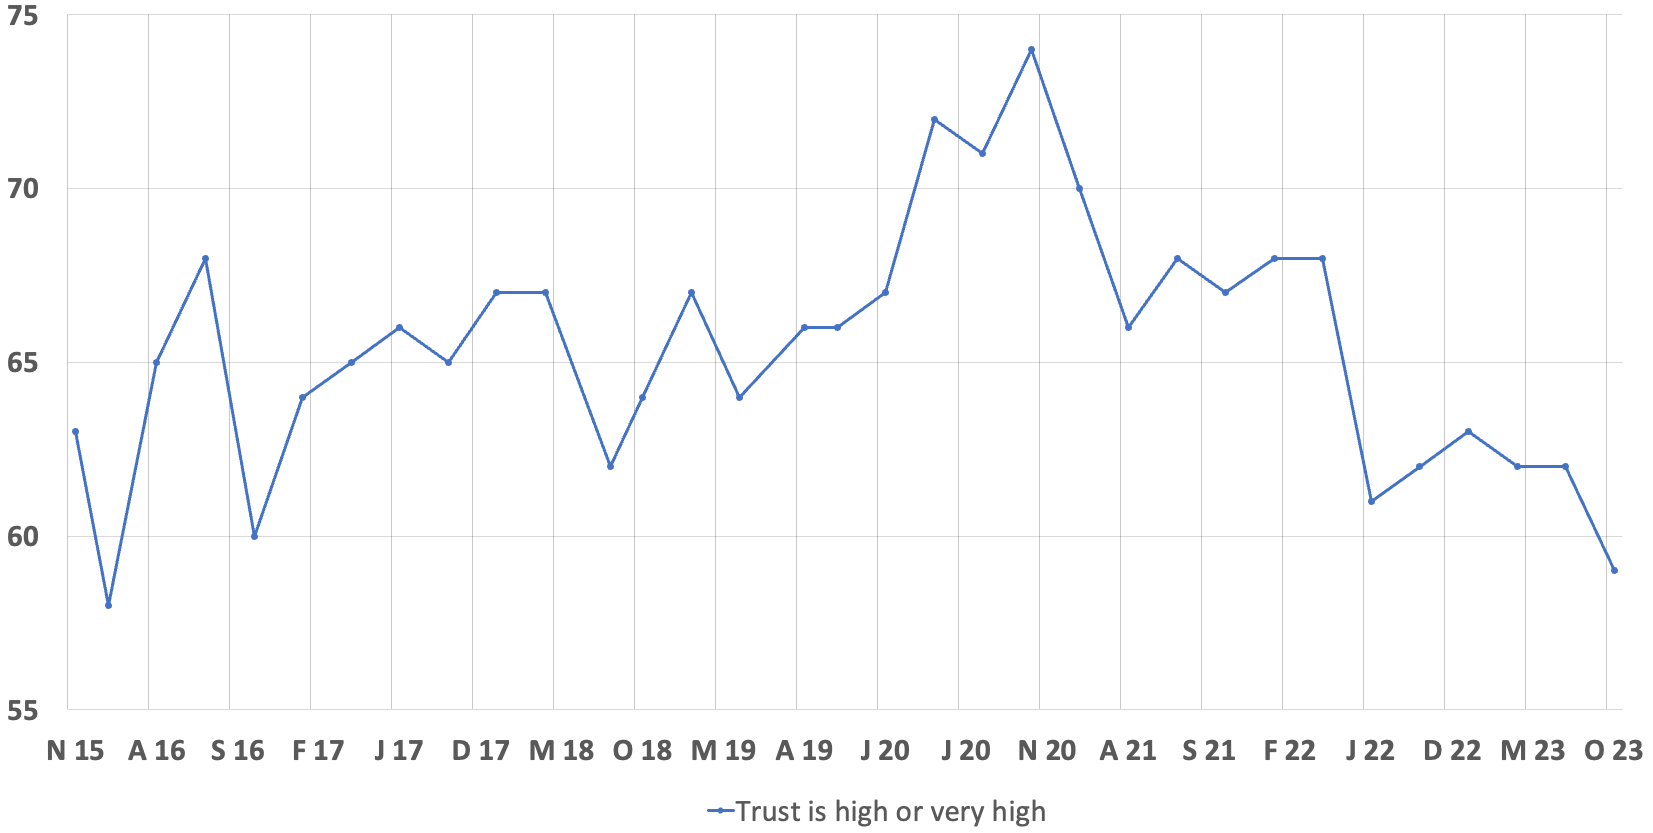
\includegraphics[width=0.8\linewidth]{./graphics/images/FGW-Trust-in-ARDZDF.png}
  \caption{Question: How high is your trust in \gls{psm} ARD \& ZDF? (2015-2023) \cite{zdf-politbarometerVertrauenGlaubwuerdigkeitBerichterstattung2023}}
  \label{fig:trust-ger}
\end{figure}

Surely its impossible pinpoint one signular event, person or technology as the starting point for trust issues towards media within a society. We chose to orinate this research from a technological view. And while we define DeepFakes as the umbrella term for all synthetically generated Fake News, we will chronologically encounter FaceSwaps first as they are the oldest (2017) of the relevant technologies. The next DeepFake tool to come around was probably wav2lip in 2020. Please bare in mind that literature published before the \gls{genai} boom of 2022 refers to DeepFakes as FaceSwaps in most cases, simply because other technologies where non-existant or irrelevant to the public until very recently. The term DeeFake was often used analogously with FaceSwaps until other technologies advanced such as synthetic voices, lip-remapping and todays image generators.

\section{Perceptions and Implications through Secondary Indicators} 
\label{sec:rel-secondary}

Investigating deepfake technology through secondary indicators, such as video comments or blog posts, is essential to comprehensively grasp public sentiment and articulate feelings surrounding this technological advancement. Analyzing these sources provides valuable insights into how individuals perceive and express their concerns, contributing to a nuanced understanding of the societal implications of deepfake technology. By looking into the diverse array of opinions presented in video comments and blog posts, we gain a more holistic view of the multifaceted landscape surrounding deepfakes.

\subsubsection*{news article reviews}
\citet{westerlundEmergenceDeepfakeTechnology2019a} provide a literature review on "emerging scholary literature" in addition to publicly available news articles. They used this data to reflect on benefits, threats and examples of current DeepFakes and how to combat them. The authors list several benefits in the regions of media production,educational media and digitalcommunications, games and entertainment, socialmedia and healthcare, material science, and various business fields, such as fashion and ecommerce. As examples they name several entertaining DeepFakes of famous actors or a museum installation that brought Salvador Dali back to life. \Citeauthor{westerlundEmergenceDeepfakeTechnology2019a} also conclude: "According to our study, deepfakes are a major threat to society, the political system and businesses[...]". They reached this conclusion based on the existance of countless pornographic DeepFakes, and multiple polical Fakes. The Obama/Peele Fake is quoted again, but also a viral video of the american politician Nancy Pelosi and another Fake of Donald Trump. The authors evaluated these videos to have had limited poitcal influencing, but they also provide two examples where they had consequences. In one case from 2018, a DeepFake of Gabon's long-unseen president Ali Bongo, who was believed in poor health or dead, was cited as the trigger for an unsuccessgul coup by the Gabonese military. In the other case a viral clip from Malaysia showed a man's confession to having sex with a local cabinet minister and caused political controversy. \\
About a possible solution \Citeauthor{westerlundEmergenceDeepfakeTechnology2019a} name four fields: "1) legislation and regulation, 2) corporate policies and voluntary action, 3) education and training, and 4) anti-deepfake technology". Section \ref{sec:rel-work-counteringdf} will give further insight in some countermeasures.

\subsubsection*{YouTube Comment Analysis}
The works of \citeauthor{leeBelieveNotBelieve2021} took a different approach and move closer to the corupus delicti. They picked the top 10 DeepFake Videos on Youtube and provided a framing analysis of the audience's comments. The word \textit{framing} is important here and requires an explanation. Framing refers to how the certain information is contextiolised. Or in the words of the authors: "[...]The \textit{valence framing} effect explores how information, framed positively or negatively, may systematically affect audience responses". From the 10 most views DeepFake YouTube videos, they gathered 88.362 comments from which they chose 2.689 (3\%) randomly sampled comments for further analysis. They then analyzed how the videos were framed and afterwards looked at the framing of the comments.\\
five videos were positively framed, three were classified as neutral and two had negative framing. Regarding the comments, the authors found that there were quite distinct groups who recognized positive or negative potentials of deepfakes but rarely see both, a positive and negative side in the technology. These distinct groups were also in line with the framing of the corresponding videos. The authors conclude that the an audience is largely influenced by the framing of the video and remark that this situation might not be ideal for the education of all viewers as their opposite opinion is always missing. This is quite an easy argument to follow. Of course more shades of grey are always better for a balanced discours. However we have to add doubts about the depth of information one can extract from these comments. To make an assumption, a video comment will rarely be a detailed, dialectic thought but more of a spontanous reaction to the seen video. That said it seems hard to make a consise assessments of the viewers thoughts. \\
Nonetheless the findings remains interesting to remind us that a balanced coverage of such a delicate topic is important.

\subsubsection*{Reddit sentiment Analysis}
Similar to the works of \citeauthor{leeBelieveNotBelieve2021}, \citeauthor{brooksPopularDiscourseDeepfakes2021} qualitatively investigated the framing of deepfakes, but instead used posts from the platform Reddit. In contrast to the previously mentioned analysis of YouTube videos Brooks' work is not as details in regards of specific numbers. It is still quite interesting, because \citeauthor{brooksPopularDiscourseDeepfakes2021} chose posts from December of 2017 until February of 2018 which is exactly the timeframe and platform where and when deepfake pornorgraphy emerged. During analysis, two primary themes emerged: (1) risk to individuals by way of personal abuse and reputation decimation, and (2) risk to society in terms of war threat and societal impact. As an interesting sidenote the authors mention parallels to the rise of the internet where similar threats were asumed. To conclude, the author points to the need of various solutions for all the different problems that arise from the emergence of deepfakes. According to \cite{brooksPopularDiscourseDeepfakes2021}, personal responsibility and individual literacies are often formulated as a solution, but do not take into account differences in culture, language, or digital literacies. The author calls for sofisticated media forensics in order to detect fake material. A wish, which might not be sustainable on the long run as will be discussed in section \ref{sec:rel-work-counteringdf}. To give one example, Brooks names wrongly blinking eyes as a fake indicator. But after an imperfection has been caught by an automatic forensic system it can be used as input to further improve the fake. In the end Brooks also states the need for increased responsibility at platforms to reduce the spread of deepfakes.

% Reviews with studies on actual people
\section{Controlled studies with participants}
\label{sec:rel-studypart}

While we've explored the broader picture using secondary indicators and public discourse, it's crucial to zoom in and examine how individuals directly respond to deepfake technology. This section shifts focus to measurements with study participants, aiming to uncover detailed insights into how deepfakes impact individuals' trust, perceptions, and behaviors and make them tangible with studies.

\subsubsection*{Vulnerability to microtargeting}
Whether people indeed “fall for” deepfakes is unclear and understudied, but not unimaginable \cite{dobberMicrotargetedDeepfakesHave2021}. \citet{dobberMicrotargetedDeepfakesHave2021} particularly investigated what effect deepfakes can have when amplified through microtargeting in a fictional scenario. In a study they interrogated 278 participants to answer the research question of how the attitudes of supporters of one depicted politician's party is affected by a deepfake meant to discredit the political candidate. As a blocking variable the chose christian religious identity. By answering questions about religion the participants were placed into Christian and non-Christian Groups and then randomly served by the original video, or the deepfaked video of a Dutch-Christian-Democrats politician. In the faked version, the polititian jokes about Christ's crucifixion. The authors suspected that this scenario "would move attitudes because the politician is a prominent Christian politician and the base of his party is to a large extent Christian". \\
The authors found evidence, that the attitude towards the politician dropped significantly in the experimental groups.
Statistical evidence was also found for the hypthesis, that the microtargeted Christian group was more effected by the statements than the non-Christian group. All the results indicate, that it is indeed possible to stage a political scandal with a deepfake. Intestingly their findings differed to earlier authors, who found no effects of disinformation on political behavior and attitudes. They state: "[...] indeed deepfakes are a more powerful mode of disinformation in comparison with the false news stories studied by Guess et al. (2018) and the Russian Twitter trolls studied by Bail et al. (2020)" \cite{dobberMicrotargetedDeepfakesHave2021}.

\subsubsection*{Sowing Uncertainty}
The DeepFake FaceSwap example of Obama, voiced by Jordan Peele have been mentioned several times. \citeauthor{vaccariDeepfakesDisinformationExploring2020} conducted a person study with exactly this material. The authors tested how a sample of 2.005 participants respond to three variants of the Obama/Peele fake. They have split up the video in three separate videos. Two of them were considered to be deceptive because they don't include the reveal at the end where the deepfake is explained. Of the two deceptive videos, the first one was four seconds long and included Obama "saying" that Donald Trump is a complete dipshit. The second video was 26 seconds long and included more text. The third video contained the explanatatory part of the original video, where the fake is explained and played side by side with the actor voicing Obamas appeareance.
\begin{figure}[h]
  \centering
  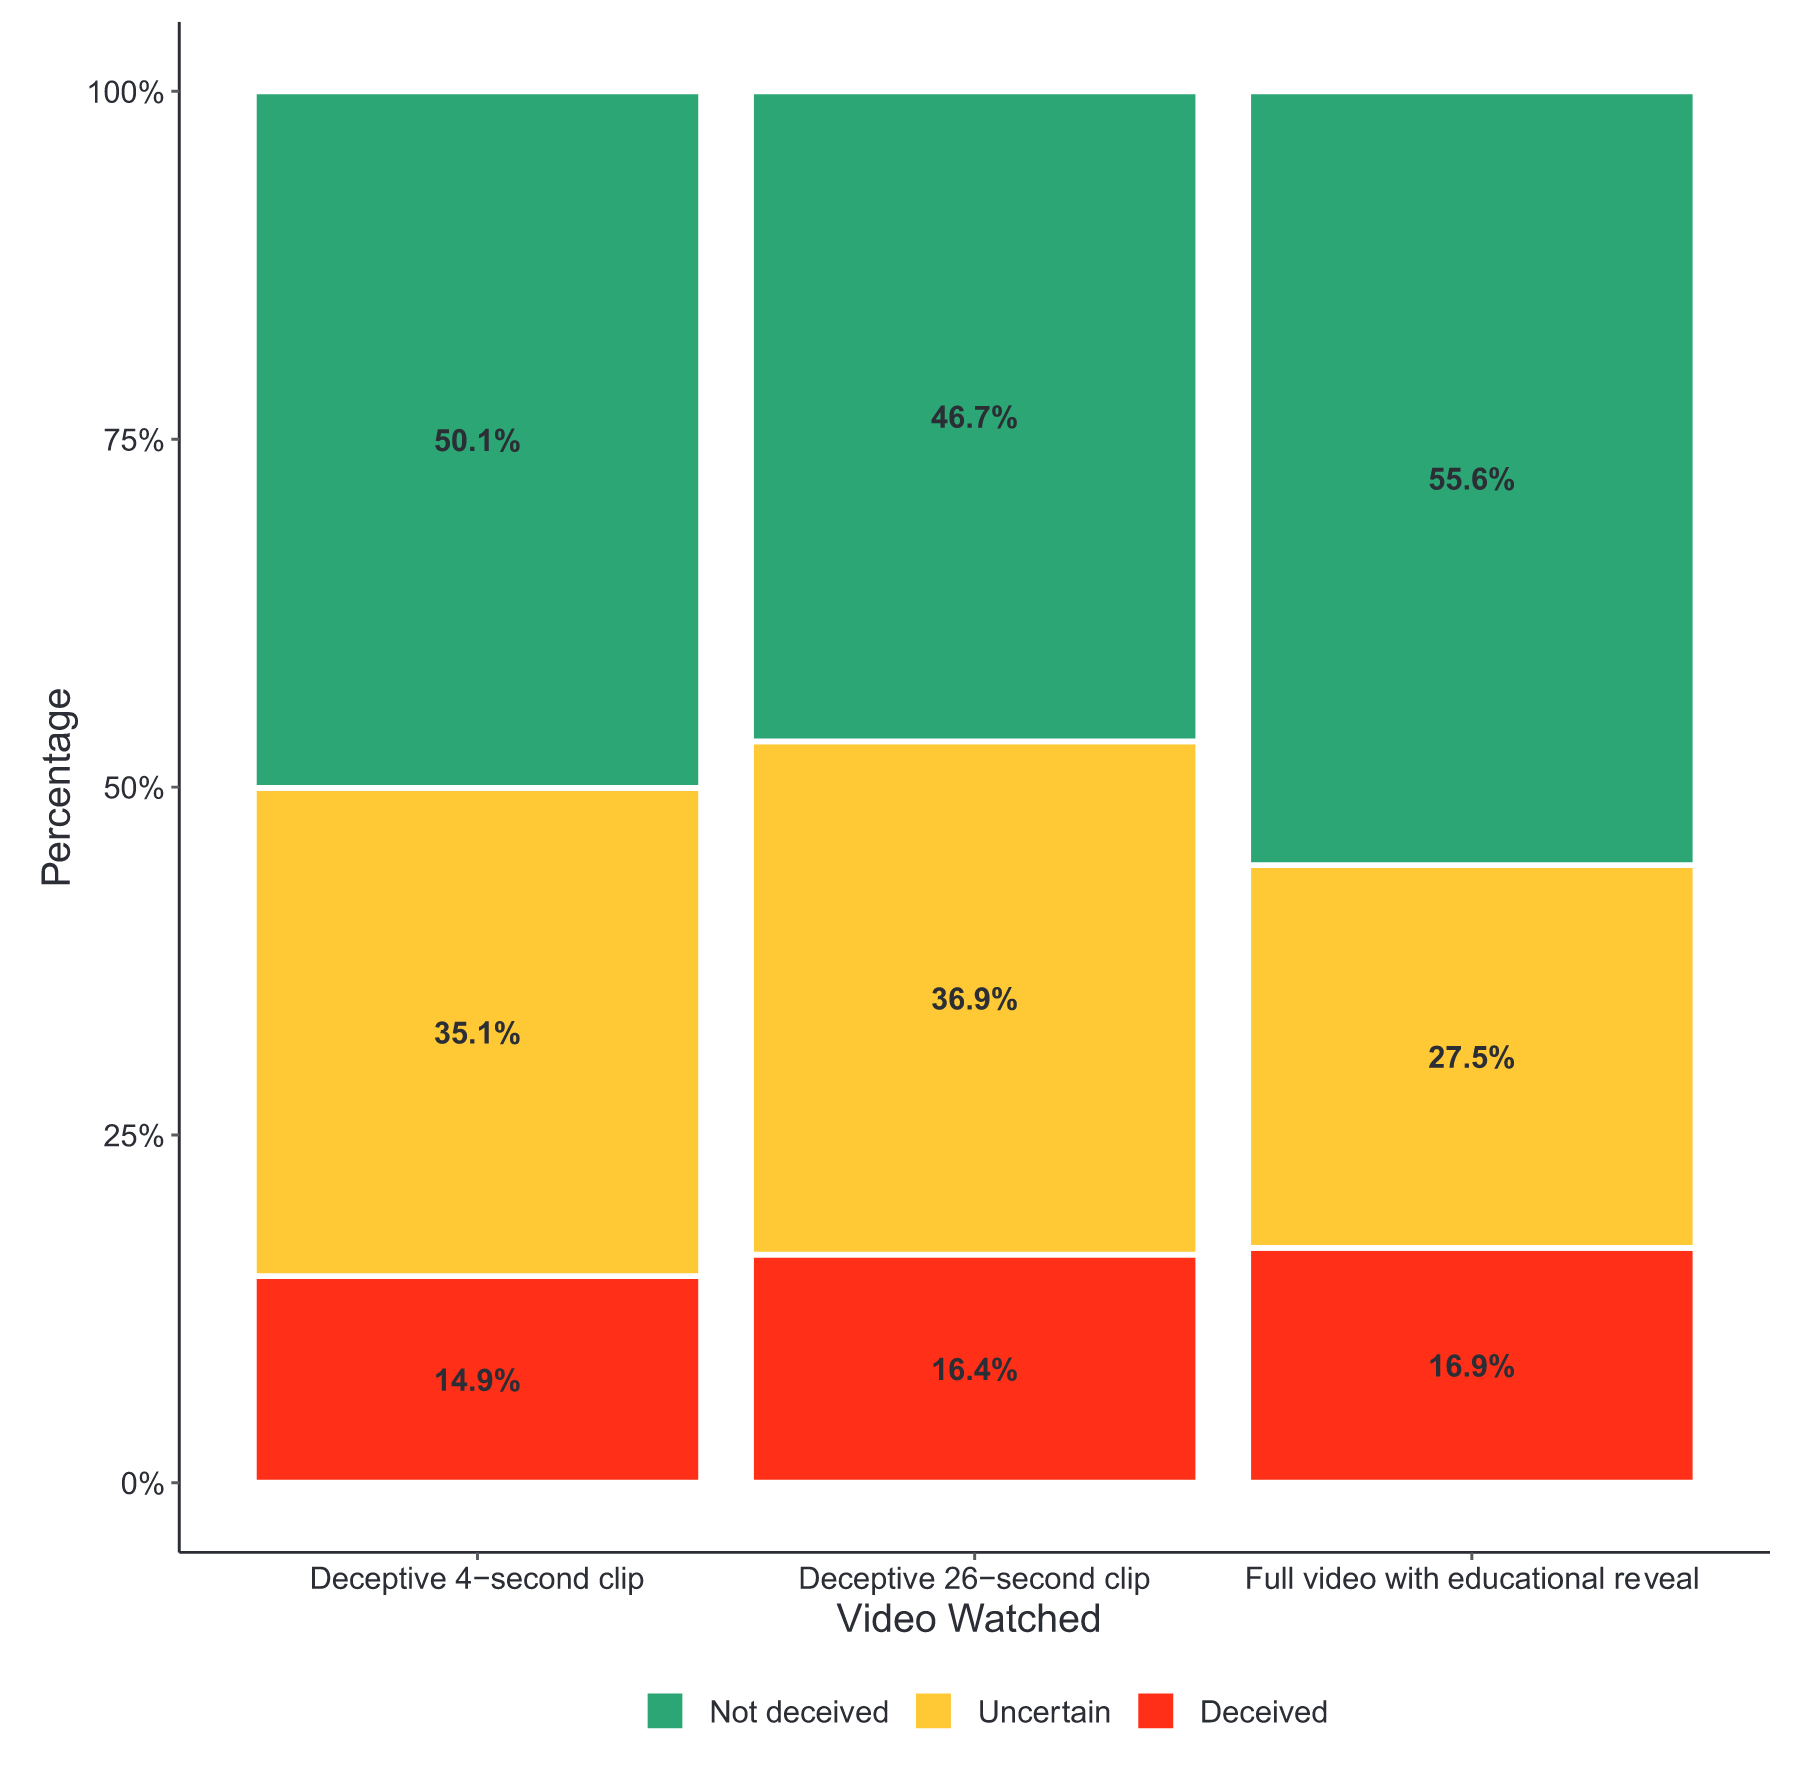
\includegraphics[width=0.75\textwidth]{./graphics/images/obamafake.png}
  \caption{Assessment of the truthfulness of the video, by treatment. \cite{vaccariDeepfakesDisinformationExploring2020}}
  \label{fig:obamafake-eval}
\end{figure}
The following results can be seen in figure \ref{fig:obamafake-eval}. The authors found that "overall, only 50.8\% of subjects were not deceived by the deepfake. This finding is surprising given the statement was highly improbable" \cite{vaccariDeepfakesDisinformationExploring2020}. 
I is also visible, that the deception rate was quite consistent over all three videos. Much more interesting was the author's second finding: "Importantly, however, the results support H2 — watching a deepfake that contains a false statement that is not revealed as false is more likely to cause uncertainty" \cite{vaccariDeepfakesDisinformationExploring2020}. \\
In an evaluation of the Obama/Peele Fake \citet{vaccariDeepfakesDisinformationExploring2020} conclude: "We have shown that political deepfakes may not necessarily deceive individuals, but they may sow uncertainty which may, in turn, reduce trust in news on social media." The authors also add, that these detrimental tendencies can lead to a downward spiral of trust loss in media and news in general. \\
In this context it is important to add that these cases might not even need manipulated video to spread fake news and uncertainty. Text can also suffice to spread misinformation, as could be seen during the Covid19 pandemic and often mentioned social media channels \cite{naeemExplorationHowFake2021}. Another awful example of how powerful just text can be, is the Q-Anon movement: \cite{zeeuwTracingNormieficationCrossplatform2020} investigated "[...] how ideas and objects travel from fringe online subcultures to large audiences on mainstream platforms and news outlets". The Q-Anon subculture has lead to several deaths in the real world (Pizzagate) and was related to the January 6 United States Capitol attack.

\subsubsection*{Uncanny valley effects}
\Citeauthor{weismanFaceUncannyEffects2021} studied the effects 3D animated talking head avatars, specifically doppelganger recreations of the participants. These 3D characters then could be used to convey messages to their real life counterpart. The messages were one pro- and on anti-AI statement recorded from the corresponding participant in advance. Using the participants' own voice, the avatar was both voiced and animated. The animation was accomplished using the software Reallusion CrazyTalk8. Two example avatars are depicted in figure \ref{fig:uncanny-avatars}.
\begin{figure}[h]
  \centering
  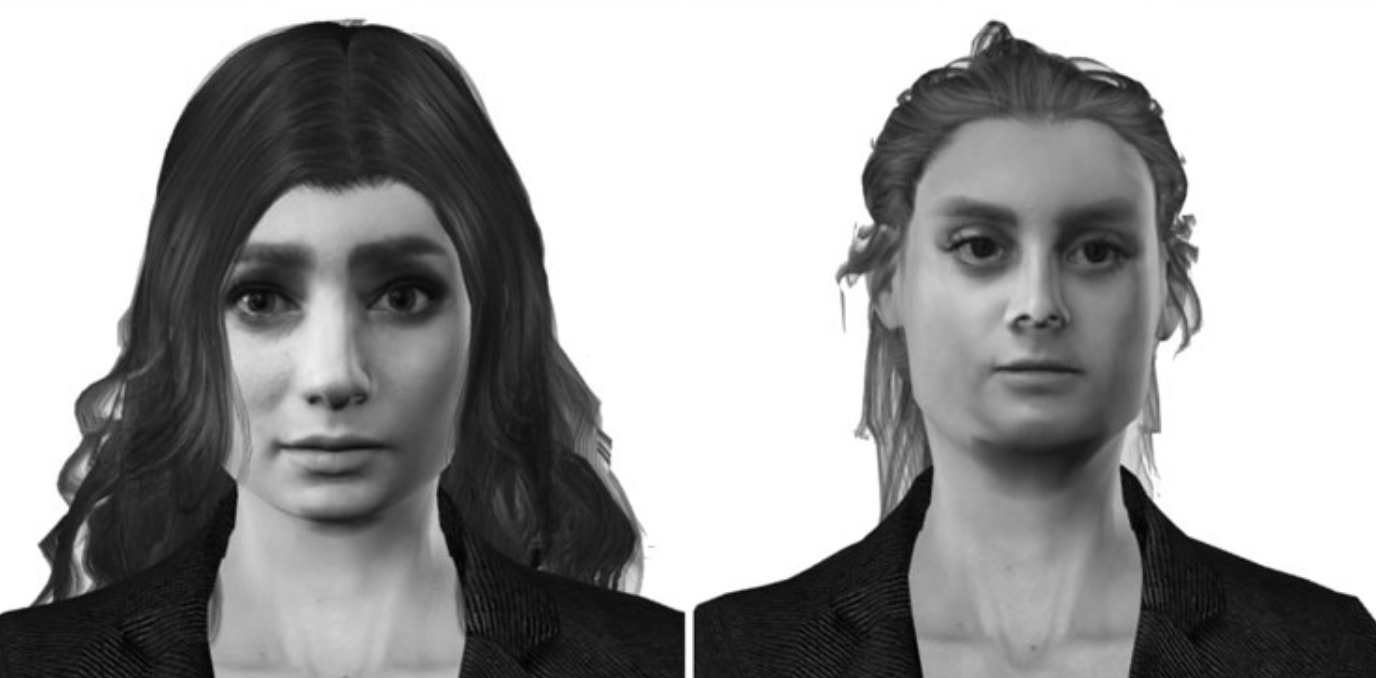
\includegraphics[width=0.75\textwidth]{./graphics/images/uncanny-avatars.png}
  \caption{Doppelganger avatars created with CrazyTalk8 \cite{weismanFaceUncannyEffects2021}}
  \label{fig:uncanny-avatars}
\end{figure}
CrazyTalk8 uses an algorithmic approach to move the targets head and lips based on audio, however it is not disclosed how the process exactly works. It is imaginable that the discrepancy between the participant's natural and real voice and the rather imperfectly looking and animated 3D character induces a significant amonunt of uncanny valley discomfort. This is amplified as the doppelgangers protrait the participants themselves, an appeareance which is very familiar. The authors willingly produced a highly uncanny perception in order to measure the trust loss due to the uncanny appeareance. In the study, some participants were exposed to their own voice and avatar (doppelganger), as well as another avatar and voice, who was unfamiliar to the participant. That way they could dial the uncanny valley feeling up and down. It was higher when the participant was subjected to its own doppelganger and lower when it was a different person.\\
The authors concluded that the uncanny valley effect mediated participant affect based AI trust. Uncanny valley perceptions were negatively related to affect-based trust. "Presenting individuals with a talking head featuring their own face decreased affect-based trust toward AIs relative to talking heads featuring a stranger's face or relative to simple audio playback" \cite{weismanFaceUncannyEffects2021}. \\
We've cited this paper, because we also introduced an uncanny vally test case a negative control group into our study (see section \ref{subsec:study design}). Different to our approach we want to remark that the study by \Citeauthor{weismanFaceUncannyEffects2021} is not suited to measure trust-issues caused by artificial intelligence technology accurately as there is no real control group that uses real footage or better AI technology (without or with less uncanny valley). We can infer, that the reduced trust is caused predominantly by the uncanny valley effect and not by the fact that it was created by AI-aided algorithms. We tried to address this study design difficulty by including real, non-fake material to be tested against in order to receive a base-line measurement of trust for real footage, free of any \gls{genai}.

\subsubsection*{Trust in synthetic Voices}
So far we have mostly mentioned papers which studied the visual part of DeepFakes. As explained earlier, this is most likely linked to the unavailiblity of easy to use, high quality audio voice clones. In the recent time this has changed. Several easy to use \gls{tts} services can be found on the internet. \Citeauthor{heiselbergAutomatedNewsReading2022} provide recent research about synthetic voices, or how they call it "neural voices". They provide a concise summary about their findings: "Results show that the participants divide into two types: the perspicacious listeners who realize or suspect that the news reading is artificially synthesized and, to some degree, are annoyed by it, and the oblivious listeners who believe the news is read by a human and are predominantly positive towards it. Participants from both groups pay particular attention to voice emotionality when evaluating the appropriateness of the neural news reader. Also, they tend to attribute human characteristics to the neural news reader. The participants single out the news messages as well as the media organization behind the news broadcast, rather than the neural voice itself as critical components constituting credibility. Transparency is of great importance when applying a neural voice in a news broadcast, since it is a prerequisite for credibility" \cite{heiselbergAutomatedNewsReading2022}. \\
For our work this is especially relevant as it set up in the environment of a news broadcast as well. In contrast to our study, it focussed on radio and the voice component alone. This reduced the surface are where the uncanny valley can act. Different to our works the authors conducted qualitative interviews instead of a quanitative analysis. To somewhat include a qualitative dimension as well, we gave our participants the option to justify their answers in free text forms. 

\subsubsection*{The disclosure of AI reduces trust}
As probably the most recent paper, we include \citetitle{toffTheyCouldJust2023} by \citeauthor{toffTheyCouldJust2023}. At the time of writing (December 2023) the cited paper has just been released as a pre-print and has not yet been peer-reviewed. \\
The authors conducted a stury using actual AI-generated journalistic content. Their focus lied on the effect of labelling AI-generated content. The studied sample consisted of audiences in the US and differnciate between polarized partisan lines. \\
They found that on average audiences perceive news labeled as AI-generated as less trustworthy, not more (see figure \ref{fig:toff-trust}). 
\begin{figure}[h]
  \centering
  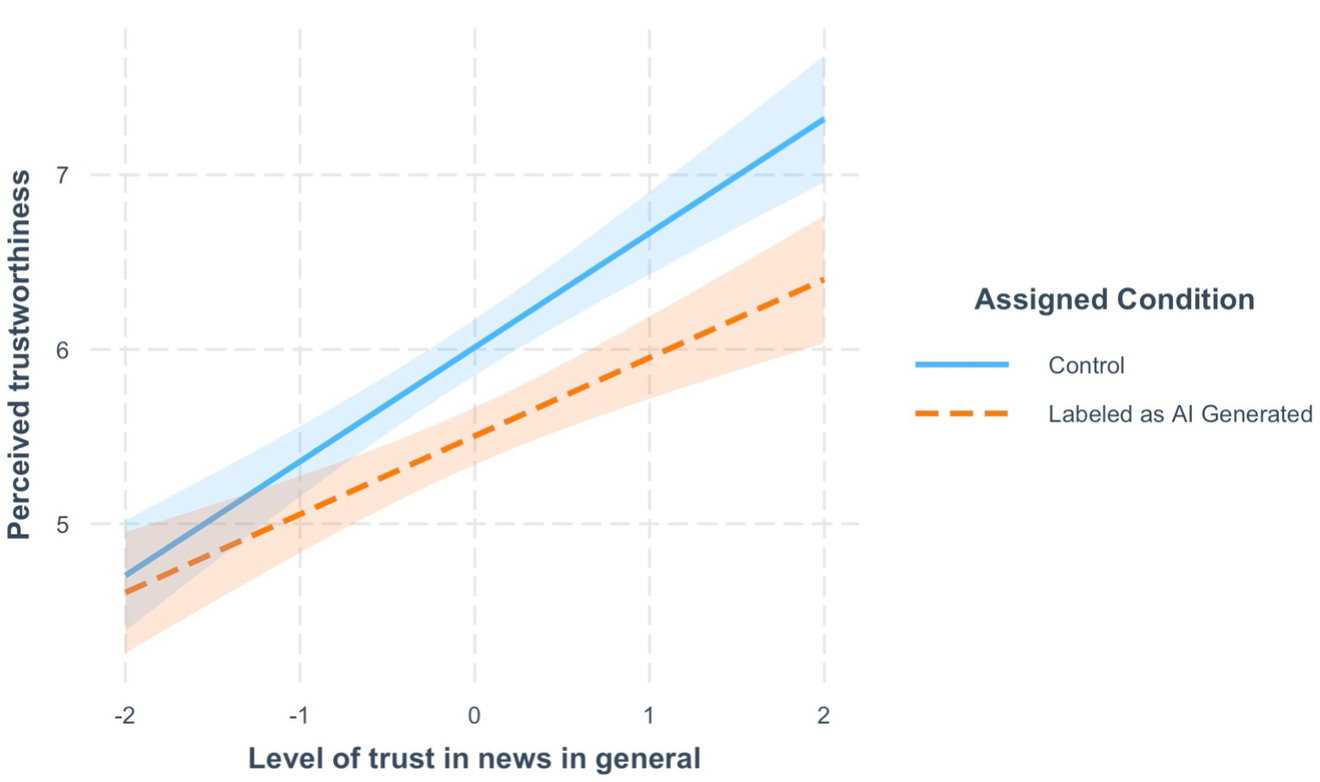
\includegraphics[width=0.8\textwidth]{./graphics/toff/Trust in news.png}
  \caption{Gaps in perceived trustworthiness associated with disclosure about the use of generative AI varied as a function of prior levels of trust in news, holding all other variables at their mean values \cite{toffTheyCouldJust2023}.}
  \label{fig:toff-trust}
\end{figure}
Furthermore, they found that these effects were largely concentrated among those whose pre-existing levels of trust in news were higher to begin with and among those who exhibit higher levels of knowledge about journalism (refered to as PNK) as depicted in figure \ref{fig:toff-PNK}.
\begin{figure}[h]
  \centering
  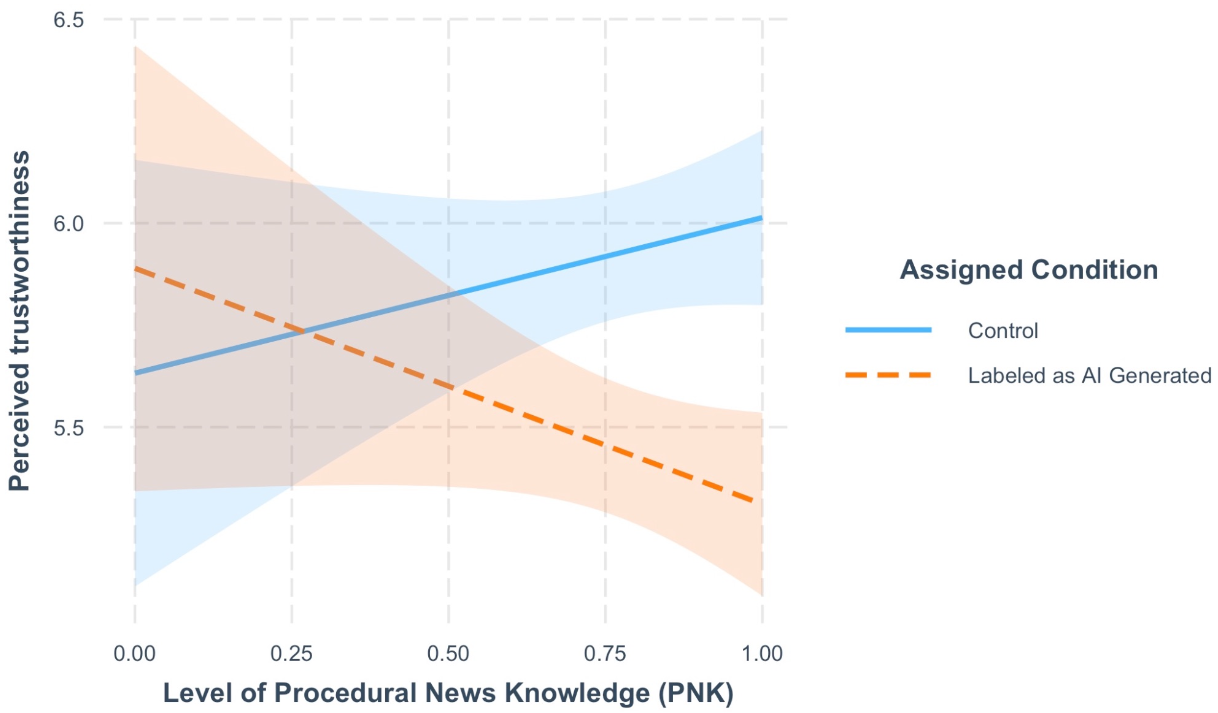
\includegraphics[width=0.8\textwidth]{./graphics/toff/PNK.png}
  \caption{Gaps in perceived trustworthiness associated with disclosure about the use of generative AI varied as a function of procedural news knowledge (PNK), holding all other variables at their mean values. \cite{toffTheyCouldJust2023}.}
  \label{fig:toff-PNK}
\end{figure}
They also found that negative effects associated with perceived trustworthiness are largely counteracted when articles disclose the list of sources used to generate the content. \\
In contrast to our work, \citeauthor{toffTheyCouldJust2023} used AI generated text as the object of investigation. This a point where our works differ, because our work had humans "in the loop" at several touchpoints. We used AI to aid the production side of how the content was conveyed, not the content itself. 
\todo{write confirmation or difference}


\section{Countermeasures}
\label{sec:rel-work-counteringdf}
\subsubsection*{Technical solutions are not Sufficient}
As soon we encountered negative usecases of synthetic media the call for efficient countermeasures arises. Since we are dealing with deep learning techniques the a frequent suggestion is to counter fire with fire and use deep learning to train a synthetic media detector. At this point it must be mentioned, that anti-deepfake technology, like forensics and AI-based detection will always have its boundries. The efficacy will always depend on the technologies ability to detect deepfakes. With better detection come better methods for generation. It's an arms race that improves both parties and gives \gls{gan} its name. \\
Because of that, other solutions in the domain of \textbf{media provinence} could provide more safety, than forensic detection. In this context, "Project Origin" has be mentioned. An alliance of media producers and broadcasters want to develop a "technical provenance approach, in conjunction with media education and synthetic media detection techniques [and] help to establish a foundation for trust in media" \cite{ProjectOrigin}. The alliance includes organisations such as \textit{BBC, Radio Canada, New York Times and Microsoft}. This lead to the creation of the \gls{c2pa}, the formulation of a technical standard to achieve to goals forumlated earlier. This project is today backed by major hardware (\textit{Canon, Nikon, Sony, Leica, Panasonic, ARM}) and software companies (\textit{Adobe, Microsoft, AWS, AVID}), media resellers distributors and providers \textit{BBC, Radio Canada, dpa, france-tv, shutterstock, universal music}. \gls{c2pa} is currently being implemented by the industry. \\
All in all, technical solutions can only contribute a minor part in solving the problem of fake news with synthetic media. The following authors have conducted research in these areas and provide alternatives to just technical solutions. 

\subsubsection*{The positive effect of media literacy}
\citeauthor{hwangEffectsDisinformationUsing2021} investigated the protective effect of media literacy education in the context of deepfakes. We have to point out that the authors use the term Deepfake frequently in their paper, but it seems that their understanding of Deepfakes is analogous to fake news. After all they do not mention deepfakes in the context of artificial intelligence once, which contributes to our understanding of their interpretation. Their study also does not use any sort of AI generated content but rather exposed the participants to fake news in textual form. Prior to the test, participants received education: General education about disinformation and deepfake-specific education. A control group which received no education was also included. \\
We still included this study as the authors were able to show that an increase of media literacy of any form has a protective effect against fake news. For our study we retrieved media literacy infromation from our participants with a separate questionaire about their media usage and familiarity with synthetic media and artificial intelligence.
\todo{confirm or differ if literacy effects resilience}

\subsubsection*{The positive effect of Priming}
Actually related to DeepFake Faceswaps is as study by \citeauthor{iacobucciDeepfakesUnmaskedEffects2021} where they tried to measure the effects of information \textit{priming} and \textit{bullshit receptivity} on deepfake recognition and resulting sharing intention. Information priming in this context is defined as "an improvement in performance in a perceptual or cognitive task, relative to an appropriate baseline, produced by context or prior experience" \cite{iacobucciDeepfakesUnmaskedEffects2021}. The priming serves the purpose of increasing the awareness about certain topics and therefore can be understood in a similar matter as the media literacy suggestions of \citeauthor{hwangEffectsDisinformationUsing2021}. \\
The amount of priming is measured against the the participants ability to recognize deepfakes (DF recognition). This was measured by asking: "The similarity of the remake to the original scene is due to the actor's abilities and not to digital video editing technologies." In adddition to the DF recognition the authors also determined a bullshit (BS) receptivity index for each participant. This index is being measured according to \cite{pennycookReceptionDetectionPseudoprofound2015}: Participants were asked to rate the profoundness of pseudoprofound sentences on a 5-point scale from 1 = "not at all profound" to 5 = "very profound" (Examples: "Your teacher can open the door, but you must enter by yourself"; "A river cuts through a rock not because of its power but because of its persistence"). Higher scores hint towards an inability to detect pseudoprofound statements. \\
Based on participants BS receptivity and DF recogntition the authors surveyed the measurements before and after priming. \\
\citeauthor{iacobucciDeepfakesUnmaskedEffects2021} summarize their results in three ways: \\
Participants in the priming condition showed greater DF recognition than the participants in the control condition. \\
Priming users with DF knowledge influences their ability to recognize a DF, but only when they are not strongly inclined to the reception of BS. \\
Their hypothesis about reduced sharing intention could also be confirmed as higher levels of DF recognition (induced through priming) reduced intention to share the video through attitudes toward the video. \\
It total "results indicate that the development of strategies to counter the deceitfulness of DFs from an educational and cultural perspective might work well, but only for people with a lower susceptibility to believe willfully misleading claims. Finally, through a serial mediation analysis, we show that DF recognition does, in turn, negatively impact users' sharing intention, thus limiting the potential harm of DFs at the very root of one of their strengths: virality. We discuss the implications of our finding that society's defense against DFs could benefit from a simple reasoned digital literacy intervention" \cite{iacobucciDeepfakesUnmaskedEffects2021}.

The listed methods all provide some degree mitigation to the deepfake problem on an individual level. At the size of a society, laws and policies should help as well. Different to public opinion, there are already laws in place which should give societal protection for both personal harm and disinformation tactics. Defamation, infringements of one's own image, privacy intrusion, these are all offenses not exclusive to synthetic media misuse. Therefore no specific AI-Act is needed to counter misuse. Because of that, we did not research lawmaking literature in this context as they are already extensively studied in other domains. The missing component to counter the threats might be the consequent enforcement of the existing laws in the virtual space. 

\subsubsection*{Literature Conclusion}
We have listed several studies about the effects of some forms of synthetic media. In regard of mitigation at the individual level, education and increasing media and deepfake literacy are efficient ways to reduce threats by deepfakes. Overall we had to realize that the available literature does rarely cover newer forms of \gls{genai}.
We conclude that research involving \gls{genai} created media is still scarce. This is understandable due to the novelty of the technologies, their complexity and the availability of tools for creation. \\
Generative AI is advancing at such a rate that it's impossible keep all developments in sight. Research has just caught up with the outcome from FaceSwap DeepFakes which today look antiquated in the light of ChatGPT and \gls{sd}. 
It is obvious that the researching community has to continue to follow the call from \citet{hancockSocialImpactDeepfakes2021} and study. A call that the authors of this paper were happy to comply.

\chapter{Methodology}
After we have established a theoretical Background as well as an overview over existing works we will now move on to the means we took to conduct our studies. We will start with the description of the technical implementation and then move on to the actual study. Still, in order to better understand the reasons why we chose certain technologies we want to first describe one central thought in our work, the spectrum of artificiality depicted in figure \ref{fig:spectrum}.
\begin{figure}[h]
  \centering
  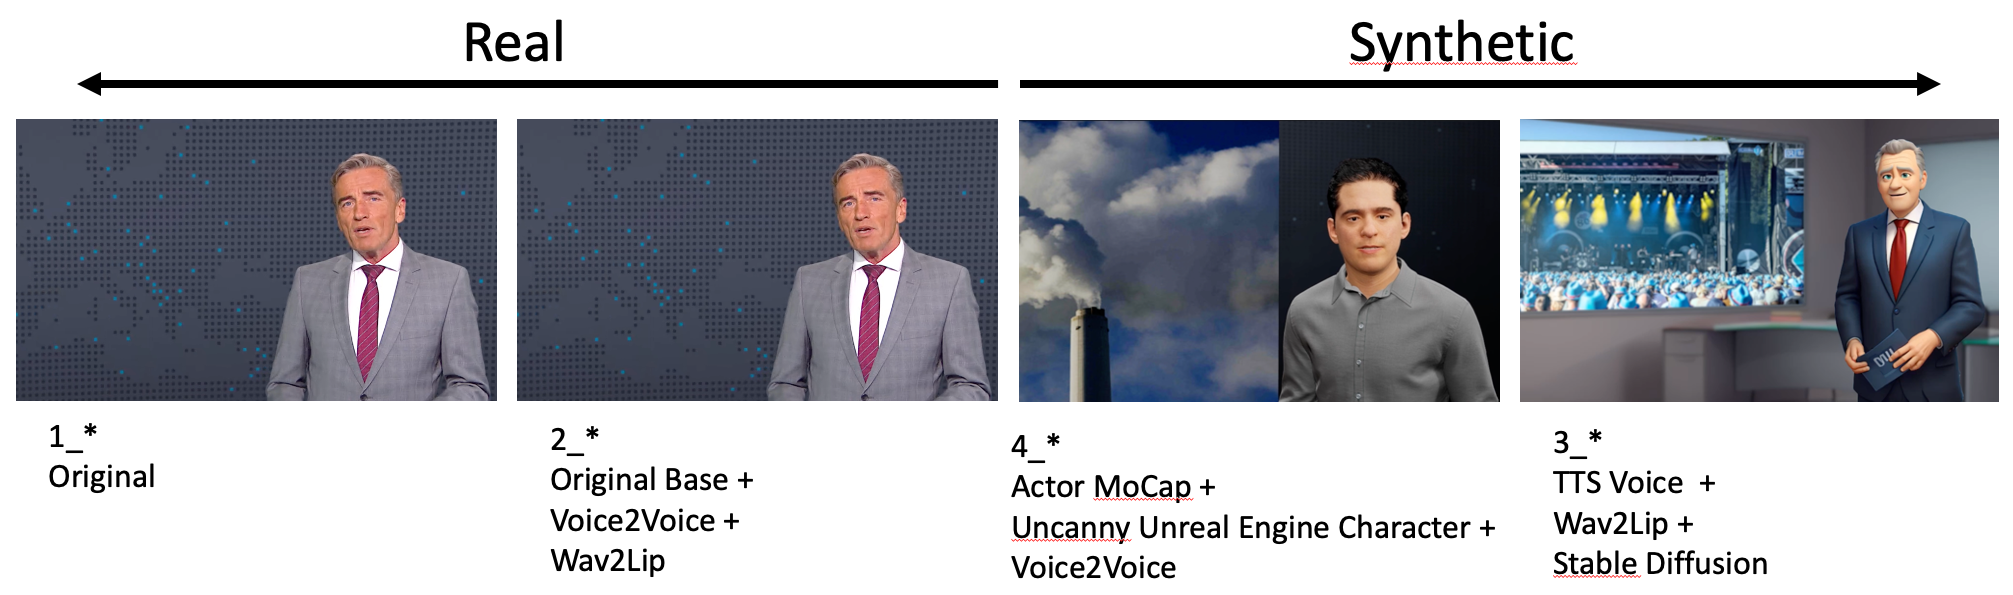
\includegraphics[width=1\textwidth]{./graphics/images/spectrum-art.png}
  \caption{Spectrum of artificiality}
  \label{fig:spectrum}
\end{figure}
On the left end, we have 100\% unaltered footage, whereas on the right end, we have a very uncanny looking, synthetic case. In between these extremes the amount of artificiality increases from left to right. The spectrum set our goals for what we wanted to create and lead to the selection of tools. A more detailed description of the thought process behind the study design will be provided in section \ref{subsec:study design}. 

\newpage
\section{implemented Technologies}
\label{implementation}
Most of the development and training has been conducted on a remote Linux Server of the \gls{hff} and film munich via SSH. Many projects featured a Gradio webui. That way, these tools could easily be accessed from remote hosts via port-forwarding. The \gls{hff} workstation featured an Intel(R) Xeon(R) Gold 6254, 128GB of Memory and a Nvidia RTX A6000 GPU with 48GB of VRAM. \\
The code was checked in at a repository via the \gls{br} at gitlab.ard.de. CI/CD was provided with a privately hosted gitlab runner. \\
During the paper, two projects were coded. The first, \gls{dvt}, provided all necessary implementations for the synthetic voices, including dataset pre-processing and training. The second is an implementation of \gls{w2l} with face upsampling using GFPGAN. Both of the projects were built in a containerized way using Docker to ease the installation of dependencies whilst working on the remote machine without root access. This also ensured high portability across systems in case we had to switch to another machine. Docker images were built with a CI Pipeline and then pushed to a private registry at gitlab.ard.de. \\
An instance of Stable Diffusion was also used without containerisation.  \\
For one of the test cases (right in figure \ref{fig:spectrum}), unreal engine was used on Windows workstation at the \gls{br}.

In the following we will give a closer insight to the generation process of several assets, such as \gls{tts}, \gls{rvc}, \gls{sd} and unreal engine.

\subsection{Voice Cloning Toolkit}
\label{sec:dvt}
While we had some previous experience in the video domain (Face swapping and Unreal Engine), we had almost none in the audio domain. Therefore we had to figure out feasible ways to create synthetic voices. There are some commercial solutions available which deliver excellent results but we wanted to see how far we can get with open source solutions. In the domain of faceswaps there are already integrated toolkits for data gathering, quality control, pre-processing and training. However this was not the case for voice cloning, which is why we decided to combine several tools into one tookit. These were CoquiTTS, an open source \gls{tts} engine (see section \ref{sec:tts}) and \gls{rvc}, which is used for \gls{v2v} generation. 

\begin{figure}[h]
  \centering
  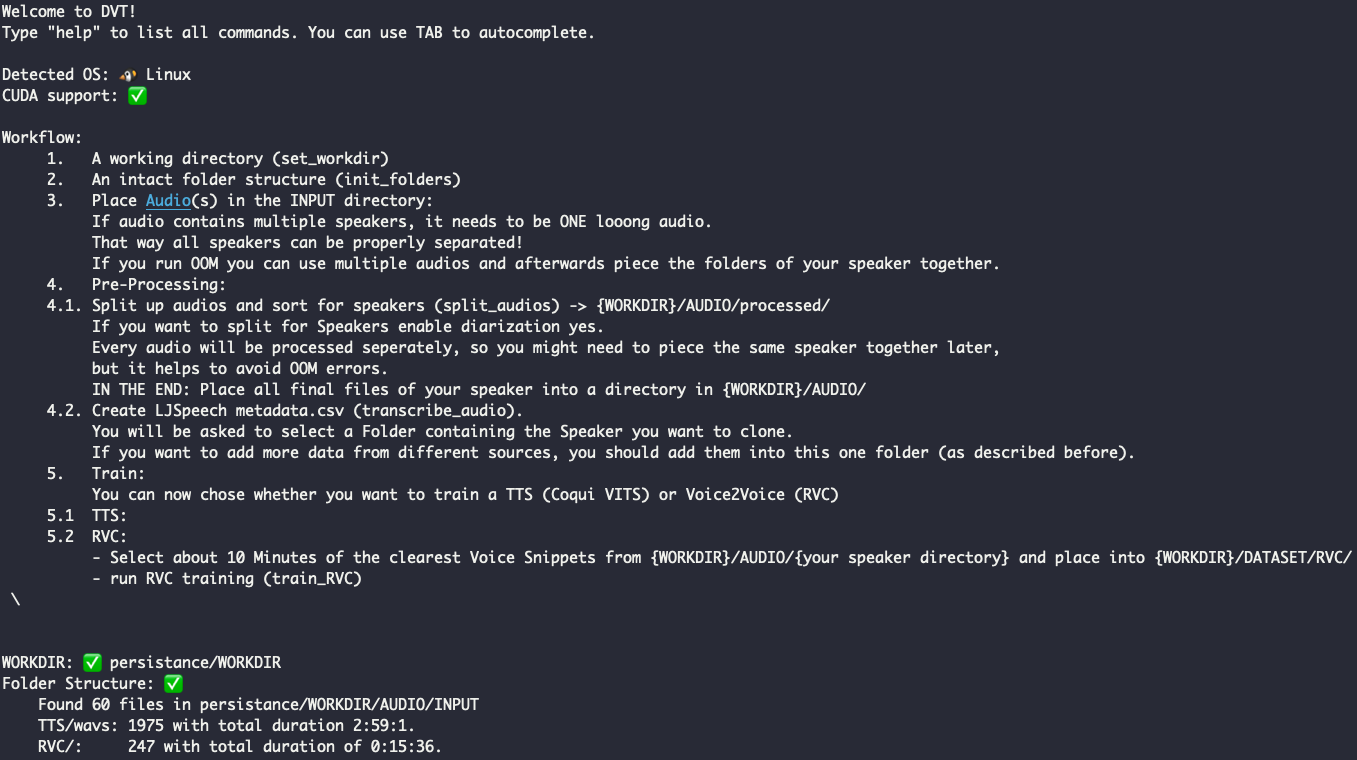
\includegraphics[width=1\textwidth]{./graphics/images/dvt-screen.png}
  \caption{Start screen of "Danilo's Voice Toolkit" DVT}
  \label{fig:dvt-interface}
\end{figure}

\gls{dvt} is a command line interface (see figure \ref{fig:dvt-interface}) and serves as wrapper for CoquiTTS and \gls{rvc} and adds methods for importing raw training data and preprocessing it. \\
\gls{dvt} is launched as a docker container with several forwarded ports. The current directory at launch time is considered to be the working directory for a certain project and is set as the workspace for the project. Several folders are created for storing the data, downloading required models and persisting them on the local filesystem. After the setup is done, one can start working by either placing files in the corresponding \verb|AUDIO INPUT| folder. For the case \gls{dvt} is running on a remote machine, as it was in most of our cases, we have added a web-based filebrowser into the docker container which needs to be started by calling \verb|filebrowser| in \gls{dvt}. Once it is up, we can browse to its port and explore the filesystem and upload required data. This is only reasonable for smaller datasets. In the case of our TTS Training Data (30 Gigabytes), downloading a tar archive via \verb|wget| and unpacking it was more reliable. 

In the following we will treat the production and training process of the regarding technologies (\gls{tts} and \gls{rvc}) in general, then explain the corresponding training data requirements and in the end summarize everything by walking through the whole workflow, from data gathering until training the model. Inference is almost trivial and is well documented for both \gls{tts} and \gls{rvc}.

\subsubsection{Text To Speech}
% General
CoquiTTS is a comprehensive \gls*{tts} tool which can be used as open source which can be deployed on own systems and at the same time drives a commercial variant "Coqui Studio". As explained in background section \ref{sec:tts} there are various ways to accomplish text to speech. We decided to go with the VITS model. Coqui uses so called "receipes" to set up a training run. As they are language specific, we relied heavily on the documentation of \Citeauthor{mullerThorstenVoice2023} who contributed a lot of work to advance the german language within the Coqui project.
With the receipes by \Citeauthor{mullerThorstenVoice2023} it is quite easy to get started. It goes without saying that each training has the option of extensive hyperparameter tuning but this was way beyond the scope of this paper and we therefore went with the basic settings provided by \Citeauthor{mullerThorstenVoice2023}, except that we increased the batch size to speed up training on our A6000. \\
Most of our development effort did not go into the training, but into the dataset preparation, which we will disclose in the next paragraph.

% Preprocessing need
\textbf{Data Requirements} \\
Regarding the Dataset structure it seemed simple: The central ressource for training a VITS TTS model are voice samples and corresponding transcription. We discovered from the Coqui community that around two to four hours of speech should deliver the best quality. In order to avoid \gls{oom} errors the audio needs to be split up in segments of maximum 10 seconds length. Lastly each and every clip needs accompanying text (example in figure \ref{fig:metadata.csv}).
\begin{figure}[h]
  \centering
  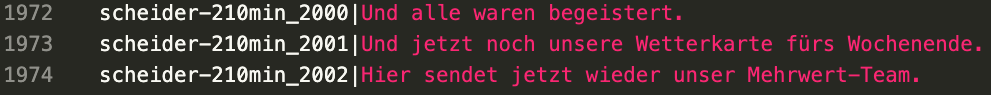
\includegraphics[width=1\textwidth]{./graphics/images/tts/csv.png}
  \caption{Excerpt of the TTS training metadata.csv file}
  \label{fig:metadata.csv}
\end{figure}
But getting to the formatted Dataset turned out to be quite time consuming with some space for automation.

% Concrete Workflow
\textbf{Concrete Workflow} \\
In the following we want to give a detailed example how we worked on our TTS Dataset. The final workflow is outlined in figure \ref{fig:dvt-tts-wf}.
\begin{figure}[h]
  \centering
  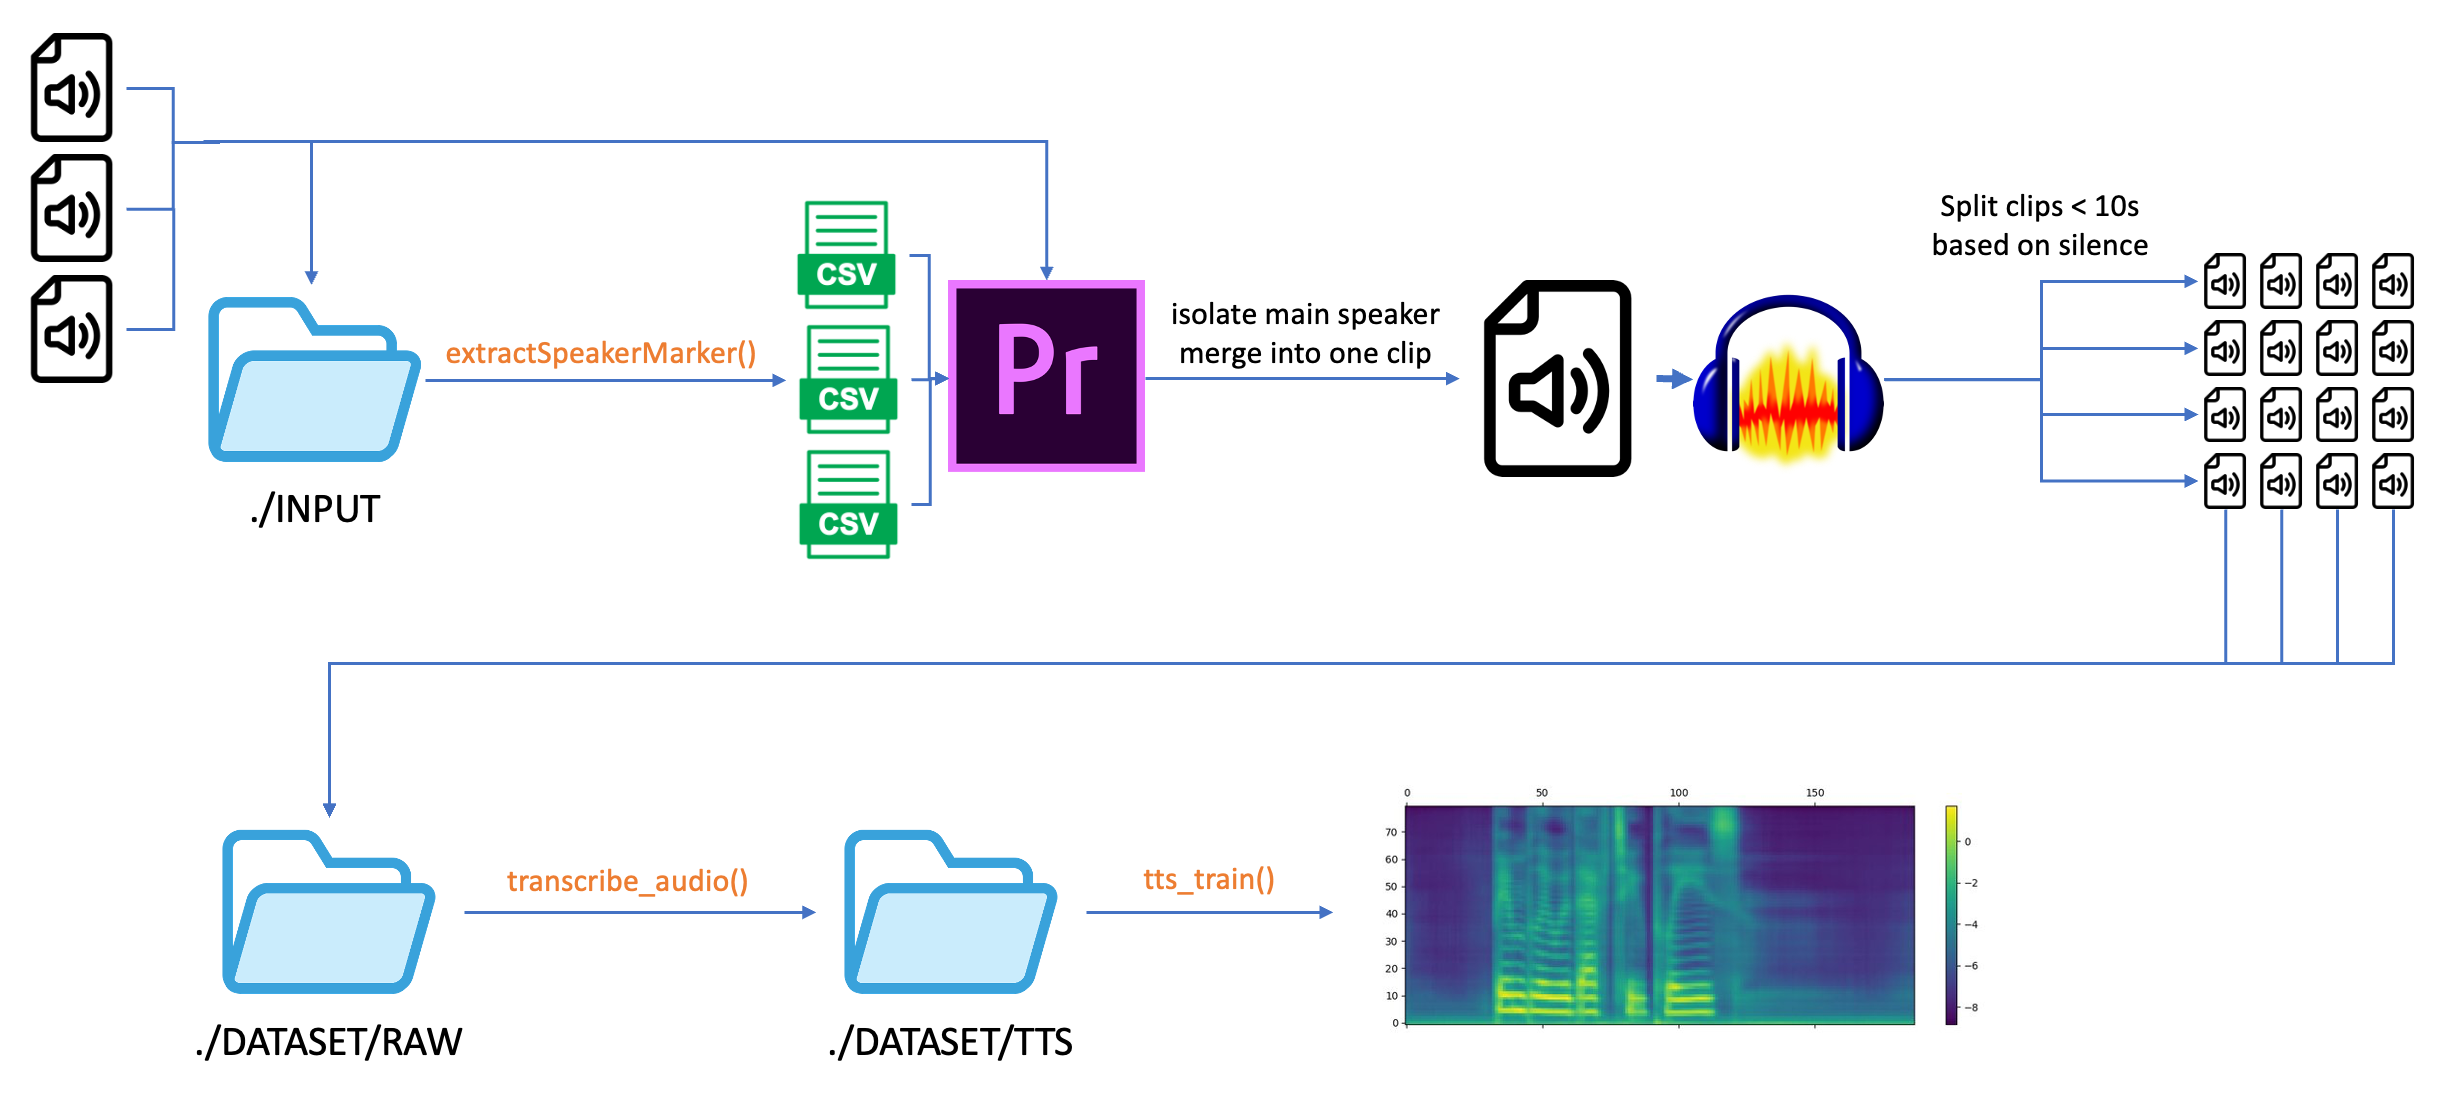
\includegraphics[width=1\textwidth]{./graphics/images/tts/tts prpro.png}
  \caption{Data preprocessing workflow for TTS training: using \gls{prpro} and Audacity for workaround}
  \label{fig:dvt-tts-wf}
\end{figure}
A good voice clone starts with a smart target selection. Therefore we had to determine a suitable environment for our test cases. As we have hinted earlier and will decribe further is section \ref{chap:study}, we chose a controled news show as the environment. TTS voices in general perform best in consistent voices where no special (emotional) intonation is required. A newscast ist perfect in this regard because of the neutral narration on the content. 
According to this requirement we aimed for four hours of speech extracted from \gls{br} news shows "BR24". We ended up with 60 shows which acounts to a total runtime of 30 hours. From each we extraced approximately 5 minutes of the anchorman's voice.\\
In the end our dataset contained 2002 individual clips with transcription. Getting there from 60 hours of news broadcast was quite an undertaking that could never be feasible without automation, which is where our partially automated preprocessing workflow comes in. \\
We used several tools to aid the dataset creation process, based of various open source projects \cite{micaAudioSplitterUsing2023}, \cite{harperEndtoEndToolkitVoice2023}: \textit{Pyannote speaker diarization} helps to distinguish multiple speakers within one audio track. \textit{OpenAI Whisper} provides audio to text transcription. \textit{NVIDIA NeMo} is used for the normalisation of the transcribed texts. To give an example numbers like "42" would get normalized to the corresponding word "forty-two". This is necessary for the training process to avoid ambiguity as all input texts are being normalized before handing them over to the \gls{tts} engine. \\
First we tried a fully automated way for the dataset creation which is depicted in figure \ref{fig:dvt-tts-original}.
\begin{figure}[h]
  \centering
  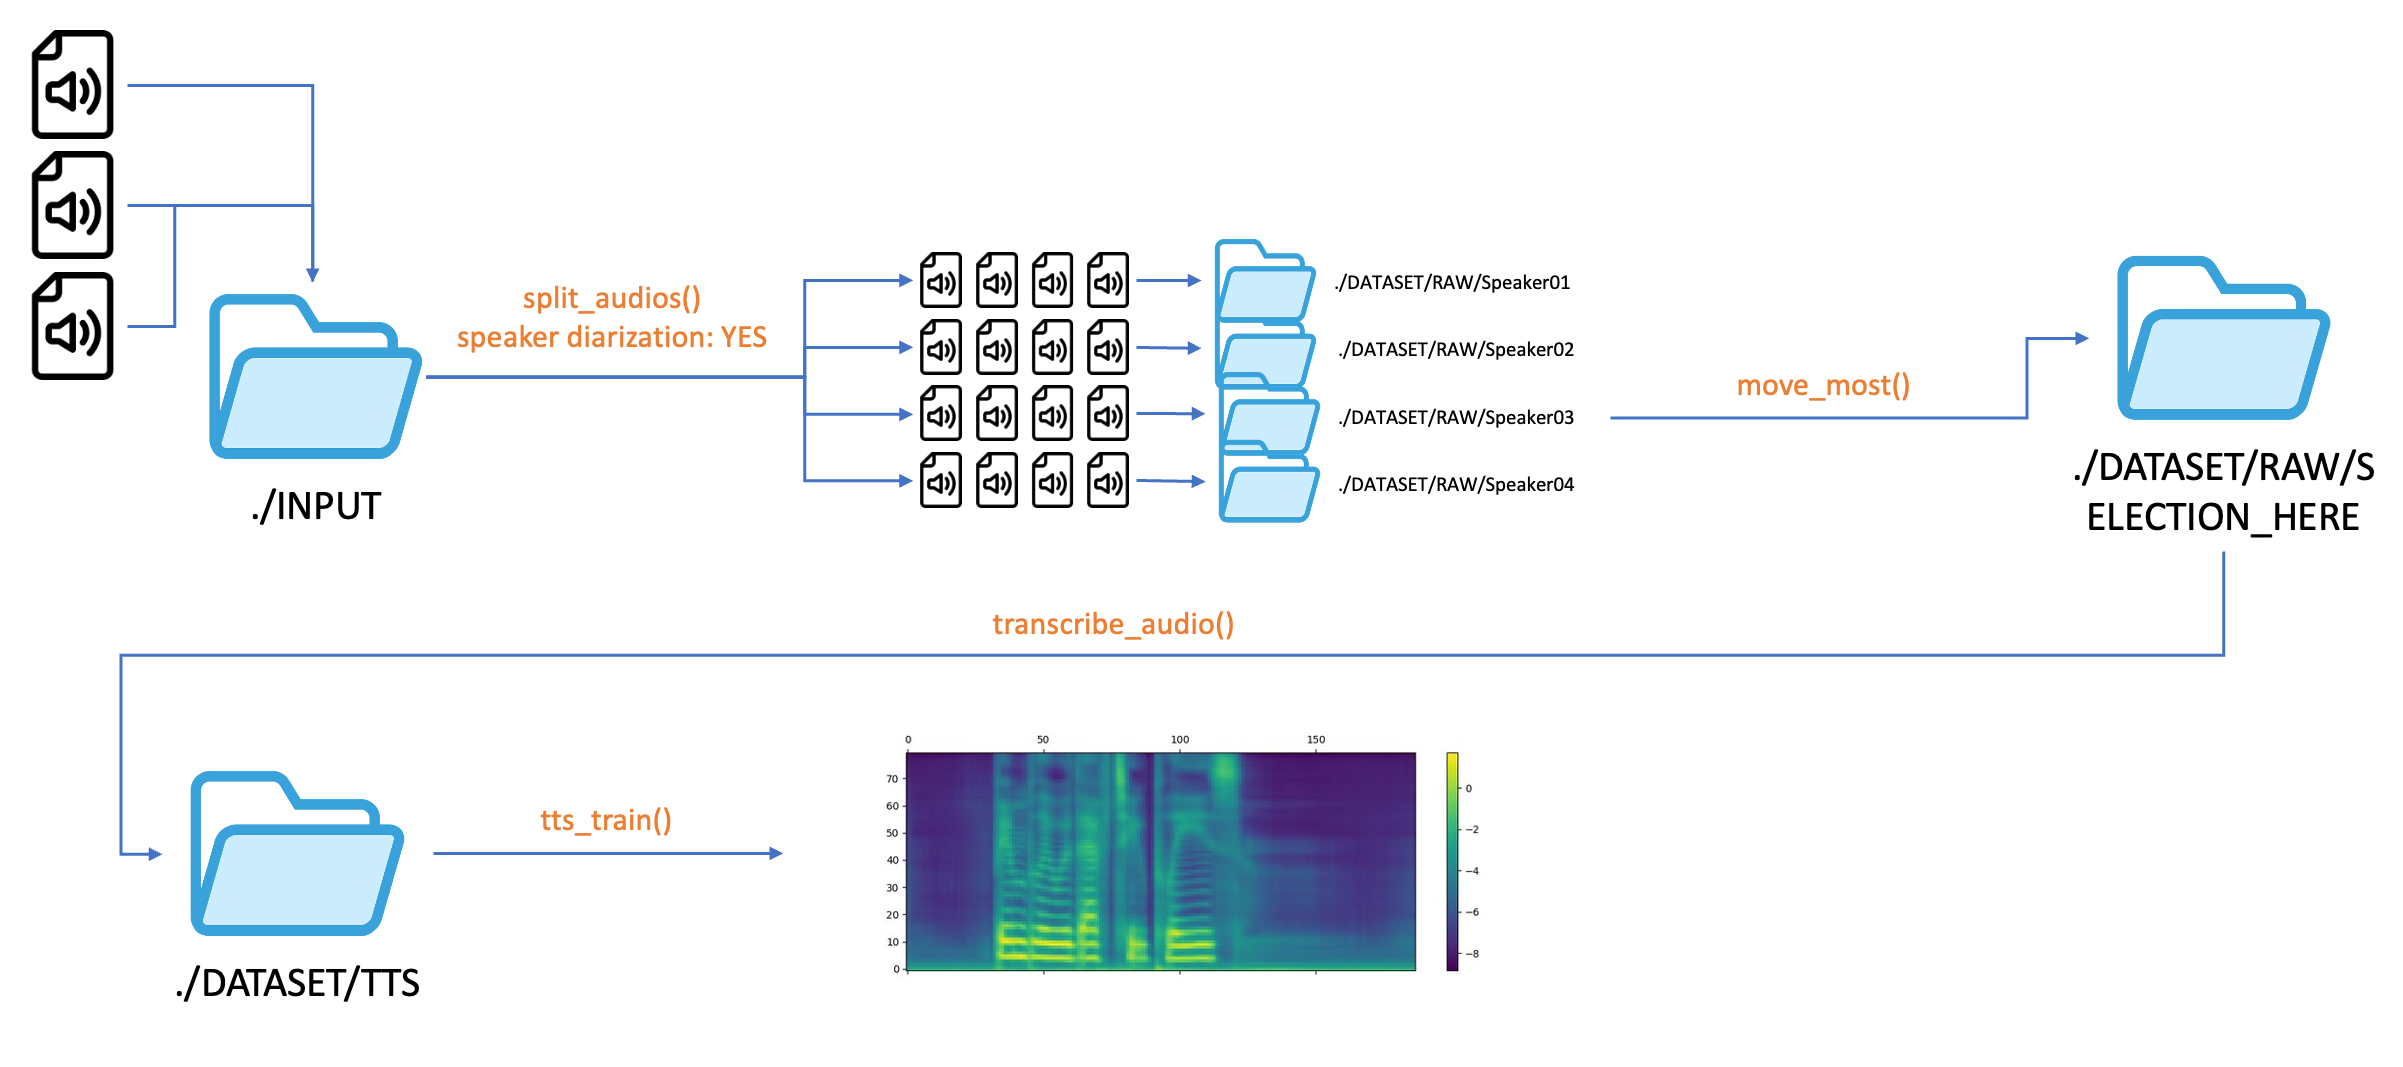
\includegraphics[width=1\textwidth]{./graphics/images/tts/tts dvt only.png}
  \caption{fully automated data preprocessing workflow for TTS in \gls{dvt} (not practicable)}
  \label{fig:dvt-tts-original}
\end{figure}
In this case we input one or multiple audiofiles and start the process. Based on the tools we've just mentioned, the audio gets transcribed and marked with a speaker ID.
It is then cut up into pieces of maximum length of 10 seconds, based on the transcription timecodes and placed in a dedicated directory based on the speaker ID. The folder with the most files, which is the folder of the anchorman's voice is moved to the TTS Dataset directory and again transcribed and receives the corresponding metadata.csv file with the necessary transcription for tts training (see figure \ref{fig:metadata.csv}). \\
This process works quite well besides rarely adding false speakers to the anchorman's directory. But there is one downside of this method which, unfortunately, makes it unusable. The transcription timecodes, provided by Whisper, which are used to cut the audios into pieces are not accurate enough and often cut parts of a spoken word away. That results in the corresponding TTS voice sounding chopped up as well. This issue could be fixed by using a cutting mechanism which relies on silence in the audio as a cutting signal instead of the transcription timecodes. Although an implementation could have been derived from one of the referenced github projects, we opted against it, because we would then lose the speaker diarization funcionality, which we needed, because our news segments contained so many different speakers. \\
Instead we opted for more time consuming manual workflow (figure \ref{fig:dvt-tts-wf}) in conjunction with the previously mentioned tools: Instead of cutting the the audios in \gls{dvt}, we added a subtitle export functionality (\verb|extractSpeakerMarker()|)for each speaker as a csv file. We then imported the subtitle files of the anchorman into the Video editing software \textit{\gls{prpro}}. Unfortunately this is not natively supported by \gls{prpro} which is why we had to rely on an extension called \textit{Markerbox} \cite{montgomeryMARKERBOXFreeMarker}. This turned out to be the quickest alternative next to reverse engineering the \gls{prpro} XML format or purchasing software. In the end we ended up with marking in the timeline (see figure \ref{fig:premier-markers}). 
\begin{figure}[h]
  \centering
  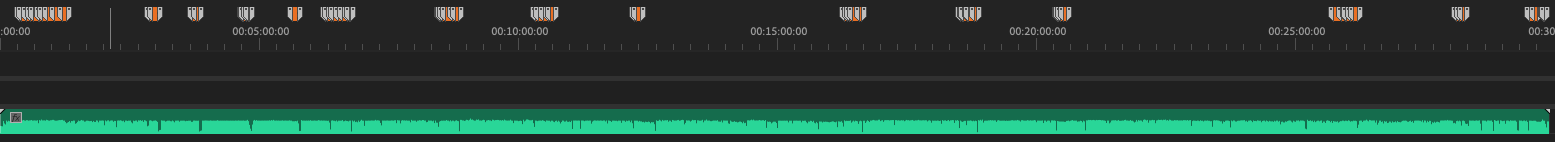
\includegraphics[width=1\textwidth]{./graphics/images/tts/premier with markers.png}
  \caption{Audio file in \gls{prpro} with markers of main speaker}
  \label{fig:premier-markers}
\end{figure}
Now we were able to manually cut aways all sections of other speakers very quickly as we had the visual aid of the markers in the timeline. Once we had isolated the main speaker we exported the audioclip. From each 30 minute news segment, we extract approximately five minutes of anchorman-only talk.\\
Next we needed to chop up the five minute piece into audios of maximum 10 seconds length based on silence detection. Though this could have been automated as discussed earlier, we didn't want to spend more time on such implementations but just get the Dataset ready as quickly as possible. Instead we chose \textit{Audacity} to confidently detect silence and render out all clips at once. \\
Now we had all clips cut out cleanly, so we uploaded them again into \gls{dvt} to finalize the dataset creating by performing one last transcription with text normalization (\verb|transcribe_audio()| to end up with a correct metadata.csv file (see figure \ref{fig:metadata.csv}). \\
Now, given that all files have been generated and placed in the right directories, starting a TTS training is rather easy. Within \gls{dvt} we invoke \verb|tts_train| and we will be guided to start a new training run with a given name and some minor parameters,like batch size and training epochs. While the training will start, a tensorboard is also spun up in the background in order to monitor the training process. It can be accessed with a web browser, if ssh port forwarding is setup properly (see figure \ref{fig:tensorboard}).
\begin{figure}[h]
  \centering
  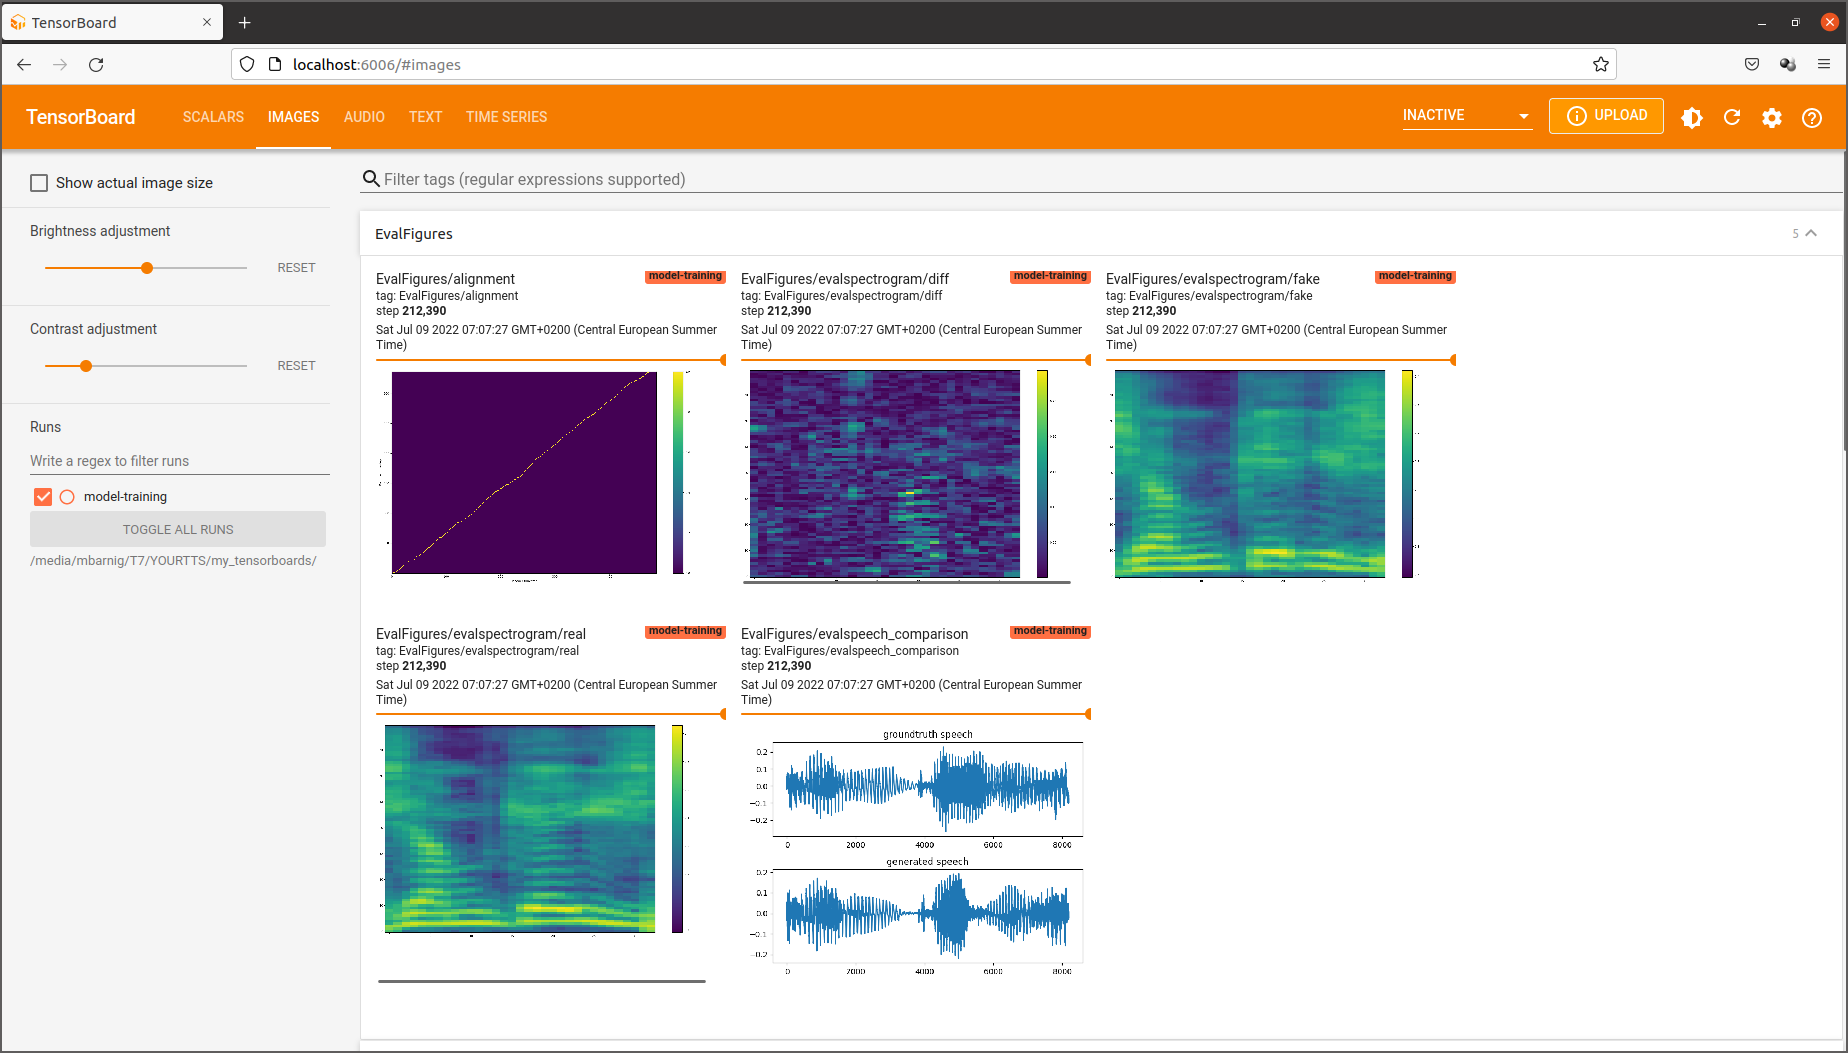
\includegraphics[width=0.8\textwidth]{./graphics/images/tts/tensorboard.png}
  \caption{CoquiTTS Tensorboard \cite{TensorboardPngMbarnig2022}}
  \label{fig:tensorboard}
\end{figure}
Tensorboard provides many interesting insights to the training process, plotting loss graphs, showing mel spectrograms and preparing generated audio files for easy playback. By judging these difference sources one can determine easier, wether the training is finished or not. 

% Inference
Now that the model is trained, inference is straight forward. For further details we encourage to check out the CoquTTS documentation. A basic CLI command to synthesize a sample looks like this:
\begin{lstlisting}
  tts --model_path "path/to/checkpoint.pth" --config_path "path/to/config.json" --out_path "path/to/outputFile.wav" --text "Text to be synthesized."
\end{lstlisting}

\textbf{Possibilities for quality improvements} \\
After the \gls{tts} Audio is generated it might be necessary to do some manual corrections to the audio track. Most imperfections are related odd sentence flow or chopped consonants towards the end of a sentence. This can be done in any editing software. We rarely had to correct anything for our model but certainly looked to cut the audio to the right positions of the video so that it matches as good as possible. \\
In addition we could also upscale the quality by applying \gls{rvc} on top of the \gls{tts} generated audios. This can not correct odd sentence flow or chopped words but add some depth to the speech quality. We decided against this improvement to have more distinctiveness between the test cases, but in a production system this might be a viable solution in order to improve \gls{tts} quality. 

\subsubsection{Voice to Voice Conversion}
%General
To convert our speech recordings to the voice of the anchorman we have used \gls{rvc}. Compared to \gls{tts}, \gls{rvc} is pretty straight forward. Regarding \gls*{dvt}, almost no adaptations to the original \gls*{rvc} \cite*{RVCProjectRetrievalbasedVoiceConversionWebUI2023} code have been made. \gls*{dvt} mostly serves as a CUDA runtime environment to provide all drivers, dependencies and AI models required to run \gls{rvc}. We added is the aforementioned \verb|filebrowser| to make file transfers to a remote GPU Server easier. Of cource, we can employ our preprocessing tools to aid the dataset generation process.\\
As depicted in figure \ref{fig:rvc-gradio}, \gls{rvc} features a Gradio user interface with several tabs in the top. Most importantly training and Model inference. For training, most hyperparameters are already set, only the Dataset location needs to be set. Inference is also done in the GUI. \\
\gls{rvc} was initially based a project for singing voice conversion, a feature which is implemented in \gls{rvc} as well. During inference voices, as well as singing voices can be converted to previously trained models. Before converting a singing voice we would need a clean vocal track. For that reason, the developers added the \gls{uvr} to a seperate tab of the GUI. With the utility the main vocals can be seperated from background music in order to convert the voice only.

%Data requirements
\textbf{Data Requirements} \\
For a good \gls{rvc} model only 10 minutes of speech are required. It is also less important than for \gls{tts} that sentences are comlete. If a word is cut of we haven't experienced any issues. Because of that we can fully use the speaker diarization and cutting process we initially built for \gls{tts}. 

%concrete Workflow
\textbf{Concrete Workflow} \\
As can be seen in figure \ref{fig:rvc-wf}, the preprocessing workflow is much leaner compared to \gls{tts}.
\begin{figure}[h]
  \centering
  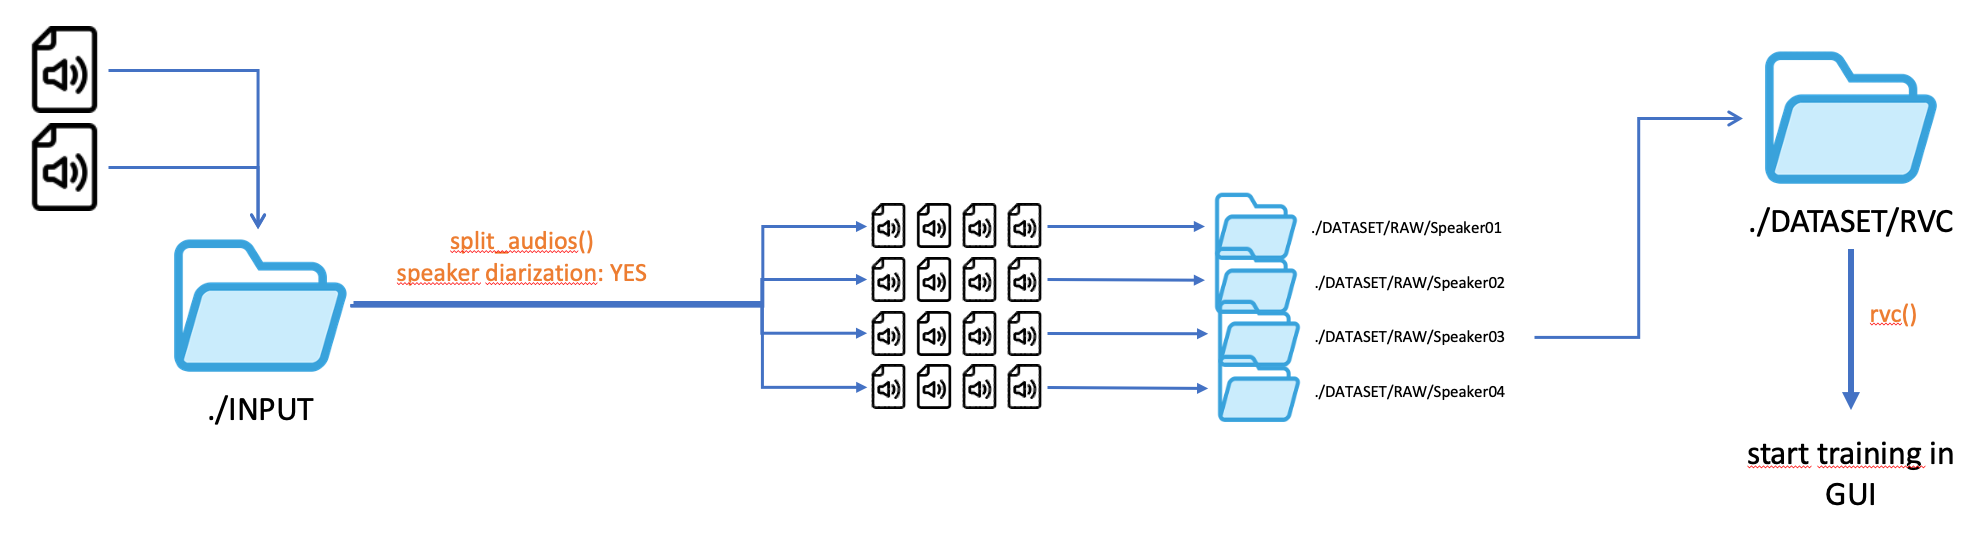
\includegraphics[width=1\textwidth]{./graphics/images/rvc/rvc-workflow.png}
  \caption{Data preprocessing workflow for RVC training}
  \label{fig:rvc-wf}
\end{figure}
As we know that we can extract approximately 5 minutes from every 30 minutes news show we need two of them for the 10 minutes training material. They get placed into the INPUT directory. Invoking DVT's \verb|split_audios| method triggers the speaker diarization and segment splitting workflow, based on a transcription and corresponding timecodes. \\
We end up with a subdirectory for each speaker of each input audio. We could now use \verb|filebrowser| to look through the speakers and listen in to the audios and then move the right audios into the \verb|/DATASET/RVC| directory. Or we can use \verb|move_most| which will go through all speaker folders and move those with most data into \verb|/DATASET/RAW/SELECTION_HERE|. Now we can move all data from here into \verb|/DATASET/RVC|. \\
Once 10 minutes of snippets all under 10 seconds are in the RVC directory we can start the \gls{rvc} UI within \gls{dvt} using \verb|rvc|. From there we can start the training by entering the dataset directory and clicking two buttons. The GUI, together with the online documentation is quite easy to understand and thus won't be explained further. This also counts for inferencing/converting voices with \gls{rvc}.

\subsection{Lip remapping}
 After we created the auditive part, we need to adjust the visual part as well. This was done, in all cases but the unreal engine case, with the help of \gls{w2l} \cite{mukhopadhyayWav2LipAccuratelyLipsyncing2023}. Similar to the development of \gls{dvt} we implemented the \gls{w2l} project as a portable docker container as well. Different to \gls{dvt} the \gls{w2l} container features a Gradio interface only (see figure \ref{fig:w2l-gradio}). This eases the file handly process as the hosts filesytem ist not required. Everything is stored inside the container during runtime and can be downloaded via the UI in the webbrowser.
 \begin{figure}[h]
  \centering
  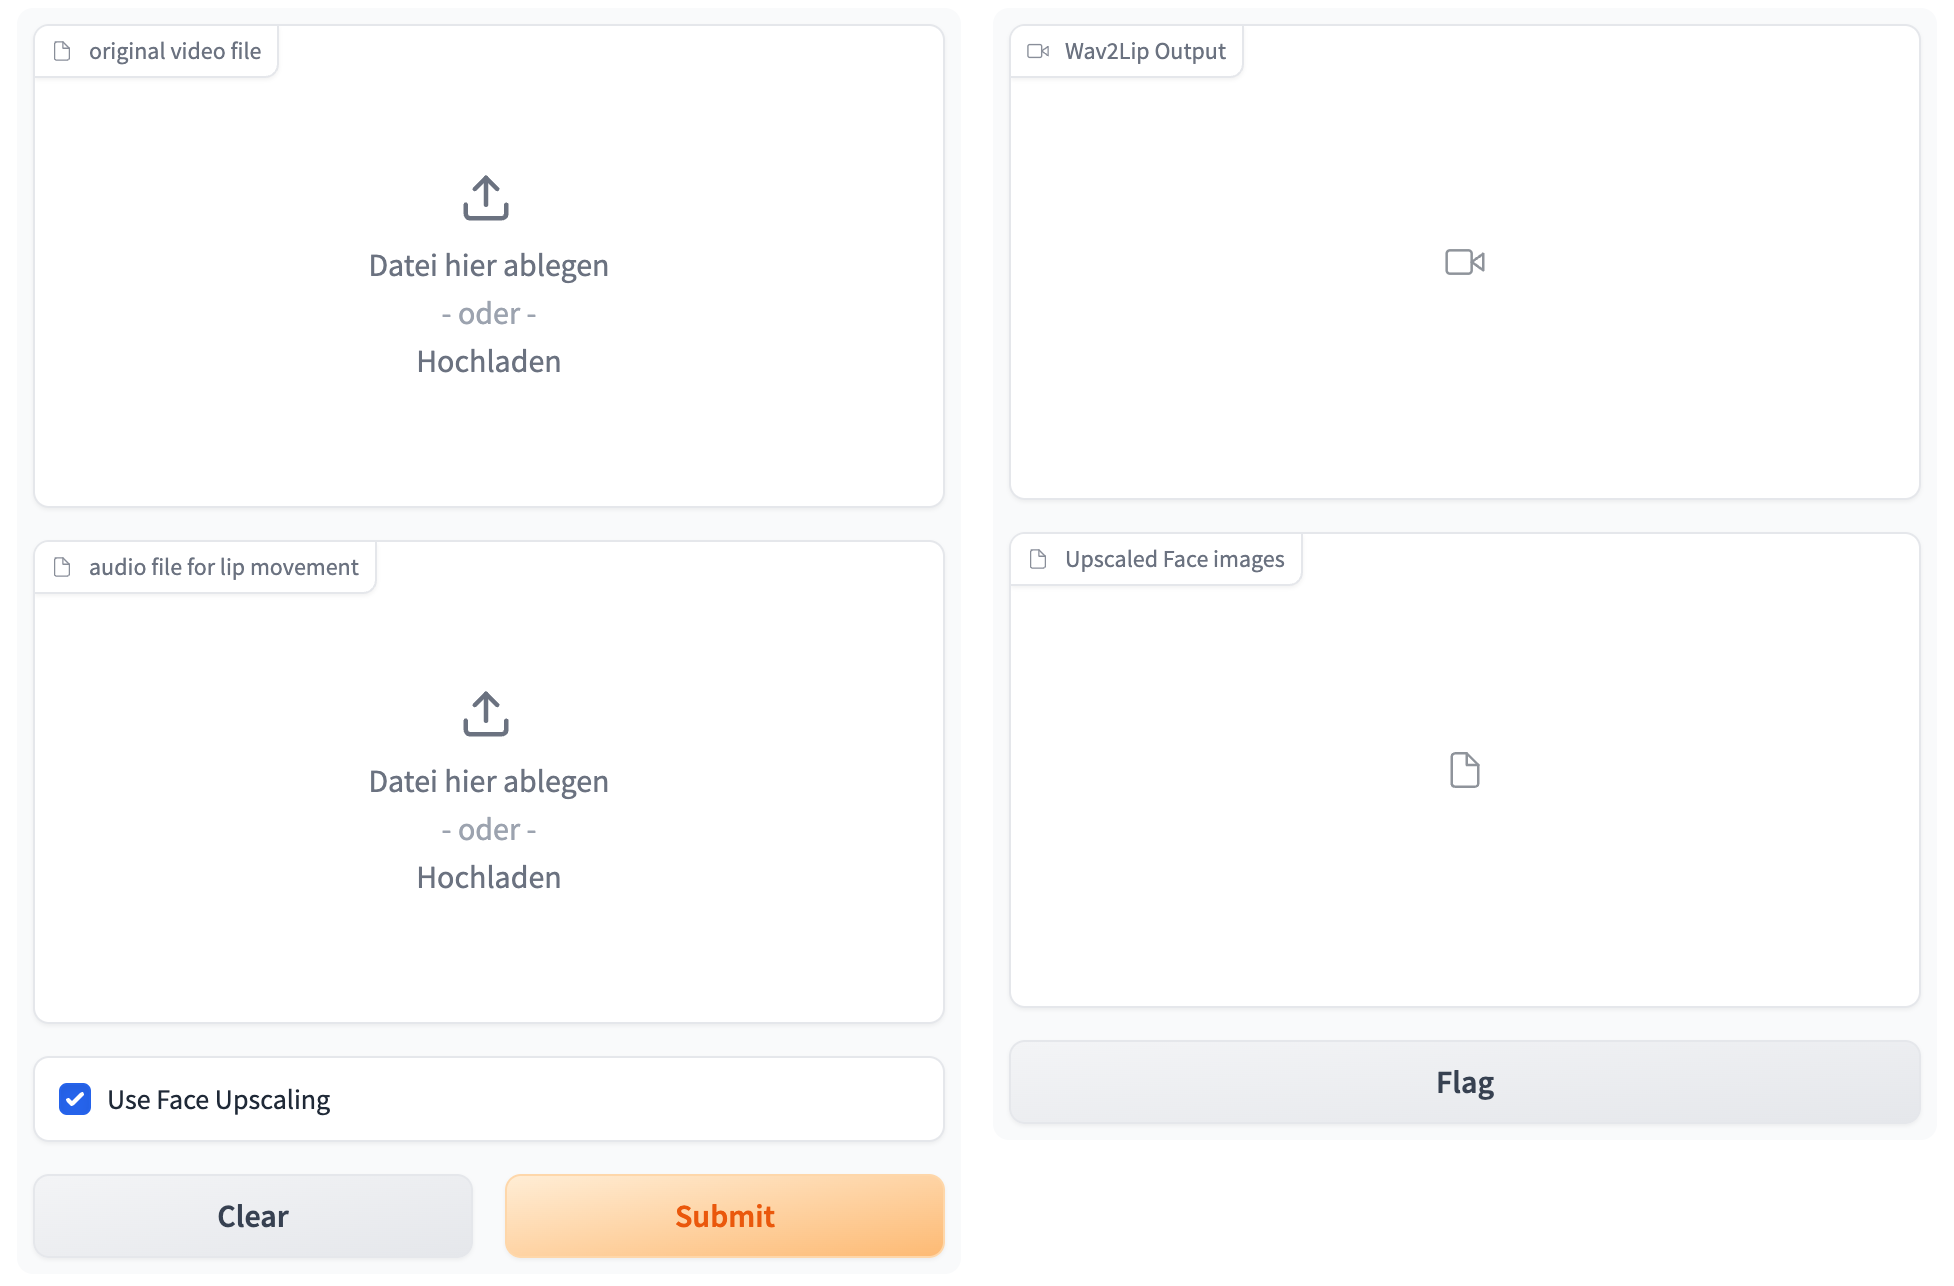
\includegraphics[width=0.9\textwidth]{./graphics/images/wav2lip/w2l-gradio.png}
  \caption{\gls{w2l} Gradio Webinterface}
  \label{fig:w2l-gradio}
\end{figure}

\textbf{Concrete Workflow} \\
The usage is fairly simple. Upload a video and corresponding audio into the interface and execute \gls{w2l}. To create best results in regards of timing, it is advised to precisely edit the audio and video beforehand so that they have exactly the same length. \\
One downside of the public implementation of \gls{w2l} is, that its lip synching model has been trained of a very low resolution of 96x96 pixels, which is not sufficient for today's standards of high definition. At a resolution of 1080p a resolution of at least 256x256 would be required. To mitigate this problem we've added a facial reconstrution library in the form of \textit{GFPGAN}, inspired by the Wav2Lip-GFPGAN GitHub project \cite{sainyAjaysainyWav2LipGFPGAN2023}.
The complete workflow is depicted in figure \ref{fig:w2l workflow} below.
\begin{figure}[h]
  \centering
  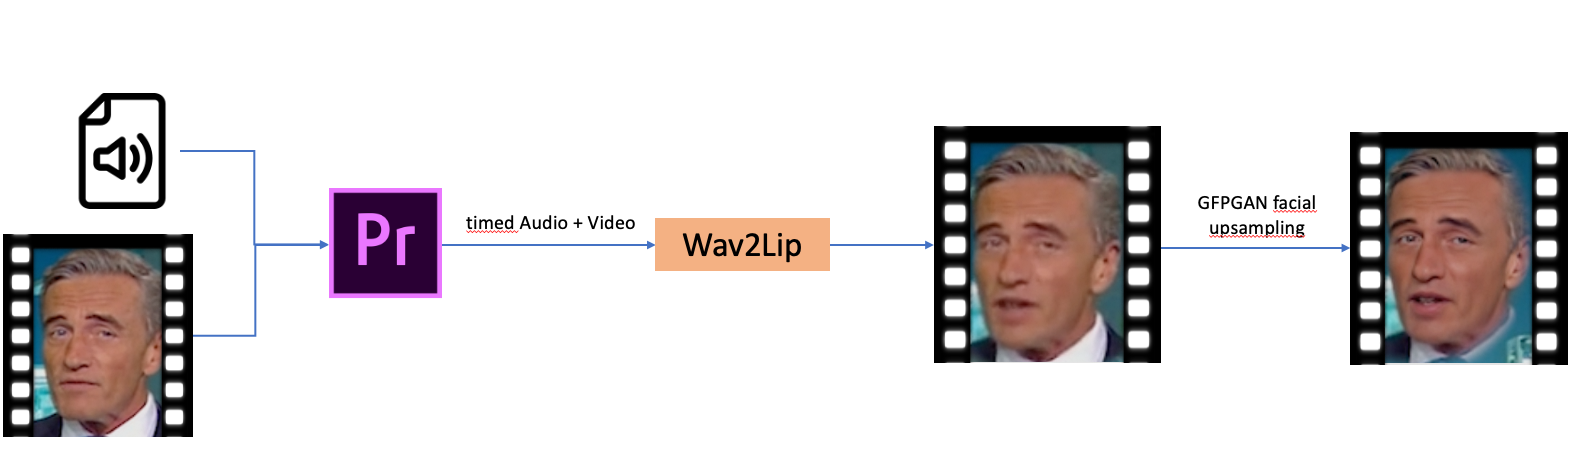
\includegraphics[width=1\textwidth]{./graphics/images/wav2lip/w2l workflow.png}
  \caption{Workflow for wav2lip}
  \label{fig:w2l workflow}
\end{figure}
Since the GFPGAN upsampling significantly increases the processing time, it can be disabled for quicker testing. Once finished, the video can be downloaded as an image sequence from to a local computer. The reason for why we chose to work with the image sequence instead of an already merged video is that we wanted to reduce the video conversion touchpoints as we lose quality with every lossy video encoding. Lastly, the image sequences and audios need to be put back together in \gls{prpro}. Sometimes minor retouches were performed in \gls{ae}.

\textbf{Possibilities for quality improvements} \\
The process of GFPGAN upsampling every frame individually introduces a small flickering effect in the facial area of the final rendering. This could be mitigated further with deflickering software but is one step we chose not carry out. \\ Alternatively to GFPGAN, it would have been possible to use the previously discussed face swapping technologies (section \ref{sec:face-swapping}) to upsample the \gls{w2l} results. We've tested the workflow using \textit{Inswapper} and the results were not satisfying: 1) Using Inswapper on top of the blurry \gls{w2l} output the result was blurry as well. It seems that Inswapper applies the blurriness to the generated image as well. This makes total sense in the case of motion blur, but is counterproductive in our case. 2) Using Inswapper on top of GFPGAN upscaled results did not work either. Still a little bit of flickering could be perceived, probably because Inswapper tries to mimic the lighting as good as possible. Also useful in regular cases, but not in ours. \\
Probably a good solution would have been to use \gls{dfl}. There are some examples on the internet which confirm \gls{w2l} in combination with \gls{dfl} as a working approach. We decided against the use of \gls*{dfl} because of the added effort for training a \gls{dfl} Model (2 weeks) and the significant post processing needed for every of our videos. 


\subsection{Stable Diffusion Video}
\label{sec:sd-video}
To further increase the degree of artificiality in our videos, we decided alienate the images with the use stable diffusion. In section \ref{sec:stable-diffusion-bg} we have established the image generator as versatile tool for many applications. The astonishing development can be credited to the active community by large amounts. For our project we've used the \gls{auto1} stable Diffusion front end with several extensions for better video processing. \\
There are two challenges with \gls{t2i}: \textit{control} and \textit{consistency}. A prompt to resemble a news anchor inside a TV studio will never remotely resemble our real anchorman. As a first, the random seed needs to be turned off. To increase the consistency at least a bit, every frame needs the same random noise as a starting value. But this cannot help us with movement of an object within the scene. In our case it is especially important that at least the lips somewhat match to the spoken audion. Luckily the \gls{sd} community had come up with a solution: ControlNet. 

\begin{figure}[h]
  \centering
  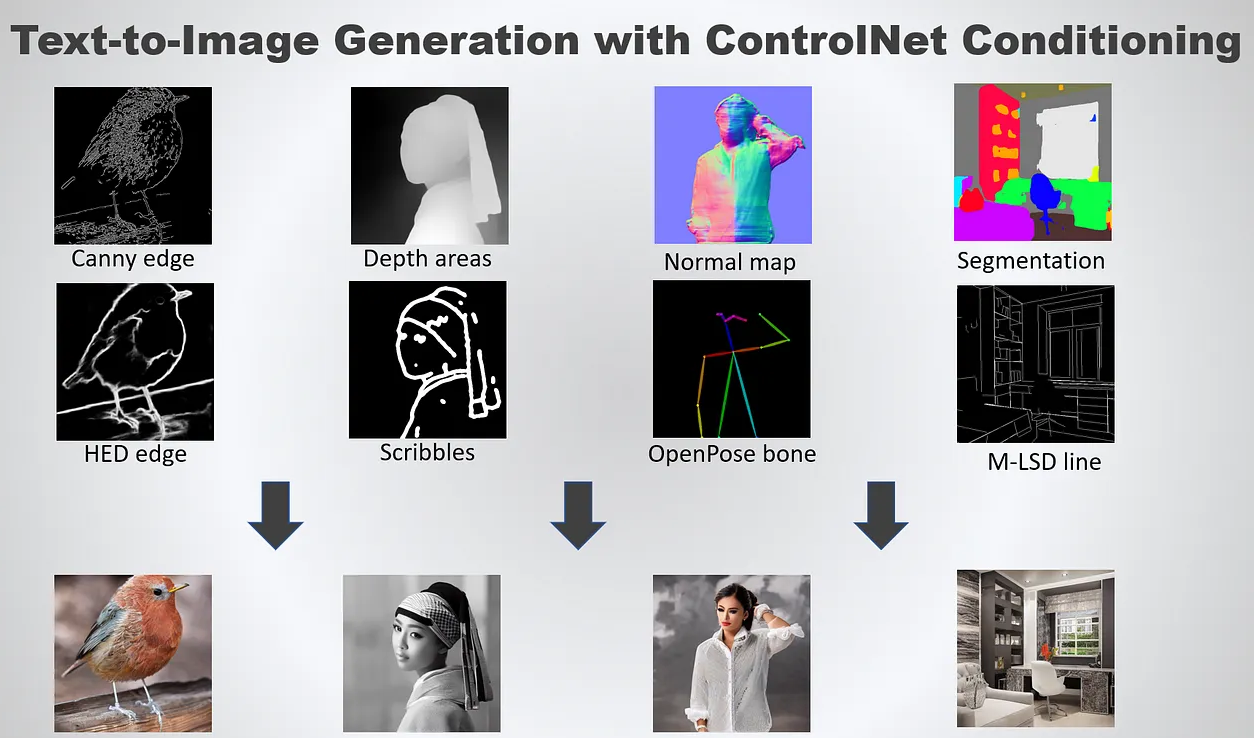
\includegraphics[width=0.8\textwidth]{./graphics/images/diffusion/ControlNet.png}
  \caption{ControlNet examples \cite{foongIntroductionControlNetStable2023}}
  \label{fig:ControlNet}
\end{figure}

In addition to text prompts, ControlNet enables the user to input additional features (see figure \ref{fig:ControlNet}) such as scribbles, various edge detection outputs, depth maps, normal maps, segmentation maps and many more. The most important controller for our purposes however was \textit{OpenPose}, which is how we created results like in figure \ref{fig:scheider-real-sd}. OpenPose extracts the gesture and facial expressions from the anchorman and feeds them into the diffusion process. For gestures and even finger movement OpenPose works quite well. Regarding the facial movement the OpenPose captures do not provide enough markers to track faces in high fidelity. Although a lot of facial expression details are lost in the process it is enough to somewhat animate the mouth and eye movement. \\
Now, after we could mitigate the \textit{control} problem we are facing the next issue. For a moving image impression we need multiple frames per second, for digital video 25 \gls{fps} to be precise. Although ControlNet helps a lot in regards of the controled categories (gesture and facial expressions) the rest of the image will look different in each frame. Also fixing the seed value does not solve the consistency issues. Figure \ref{fig:controlnet-issues} shows some of these effects.
\begin{figure}[h]
  \centering
  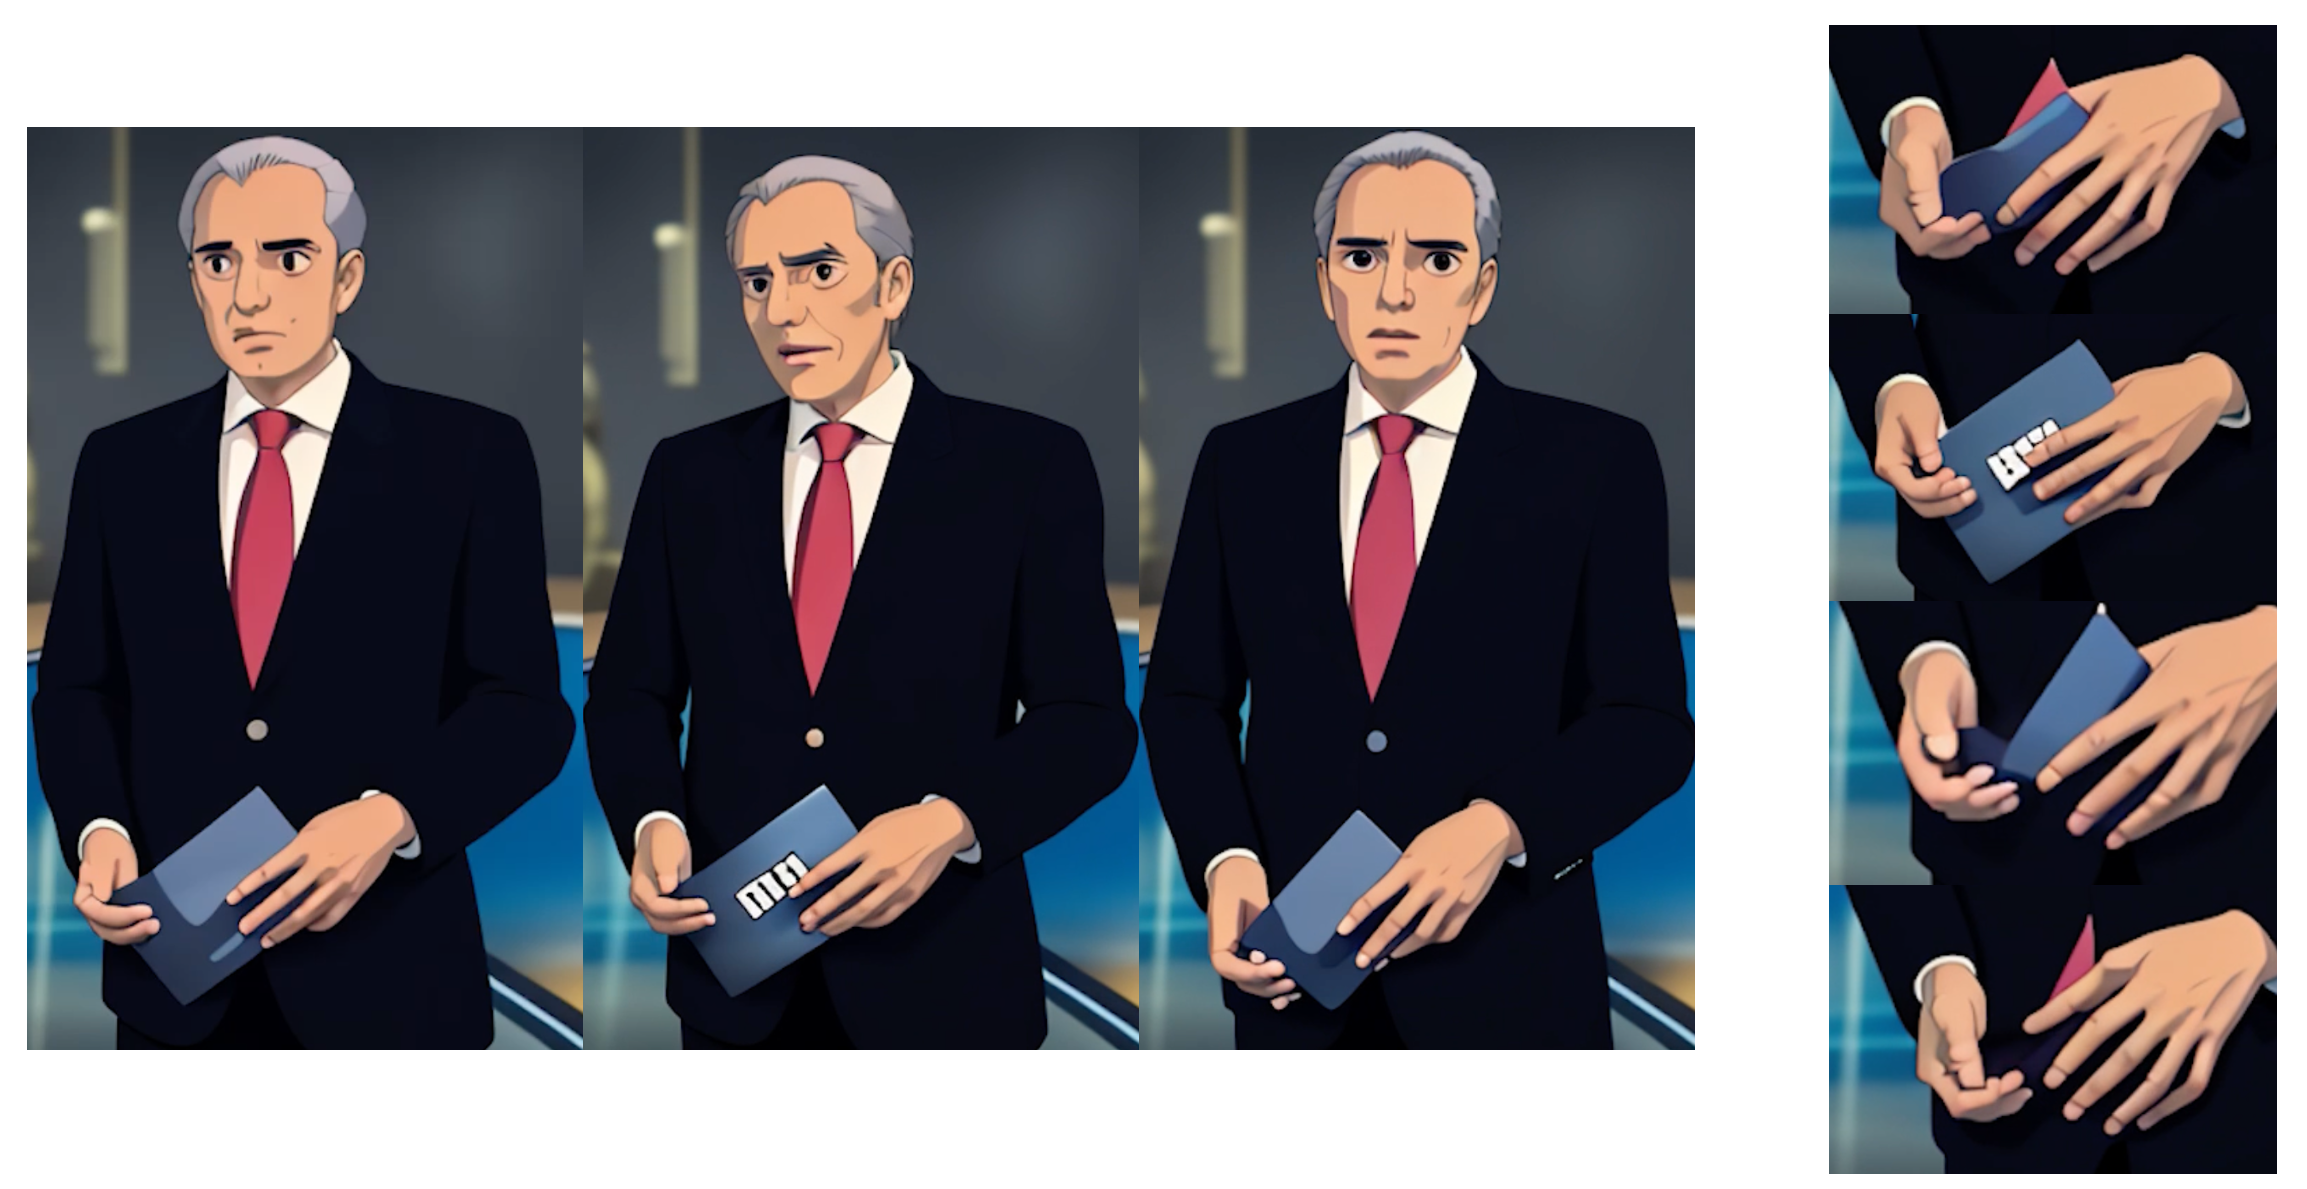
\includegraphics[width=0.8\textwidth]{./graphics/images/diffusion/ControlNet-issues.png}
  \caption{Consistency problems: Studio Ghibli LoRa, fixed seed, ControlNet OpenPose}
  \label{fig:controlnet-issues}
\end{figure}
While the posture of the hands is often okay, the card he is holding frequently changes. These effects appear everywhere in the frame, like the color of his buttons or his tie. Watching these twitches in 25 \gls{fps} is very unpleasant and greatly reduces the overall quality of the video. \\
One way of fixing consistency is by using other ControlNet layers like depth maps or \textit{Canny}. A downside of incresed ControlNet activity is reduced control using the text prompts. Consistency is also model dependent, so we tried out various models. After a lot of trial and error we ended up with the results seen in figure \ref{fig:scheider-real-sd}.

\textbf{Concrete Workflow} \\
Prior to the \gls{sd} input, the base videos were created using Wav2Lip and \gls{tts} OR \gls{rvc} as described earlier. We cropped the video to feature only the actor. This reduced processing time, increased quality and improved consistency because the area of attention was smaller and focussed. \\
After having generated the main actor we composited him to the final clip using \gls{ae}. Because the background was  twitching as well, due to consistency issues we decided to key it away, as only the actor is important for the scene. We accomplished this by generating a depth map with \gls{auto1} and using the map as the isolation criterion. Afterwards we composited the actor on a studio image background. The complete \gls{sd} workflow is depicted in figure \ref{fig:sd-full-workflow}. 

\begin{figure}[h]
  \centering
  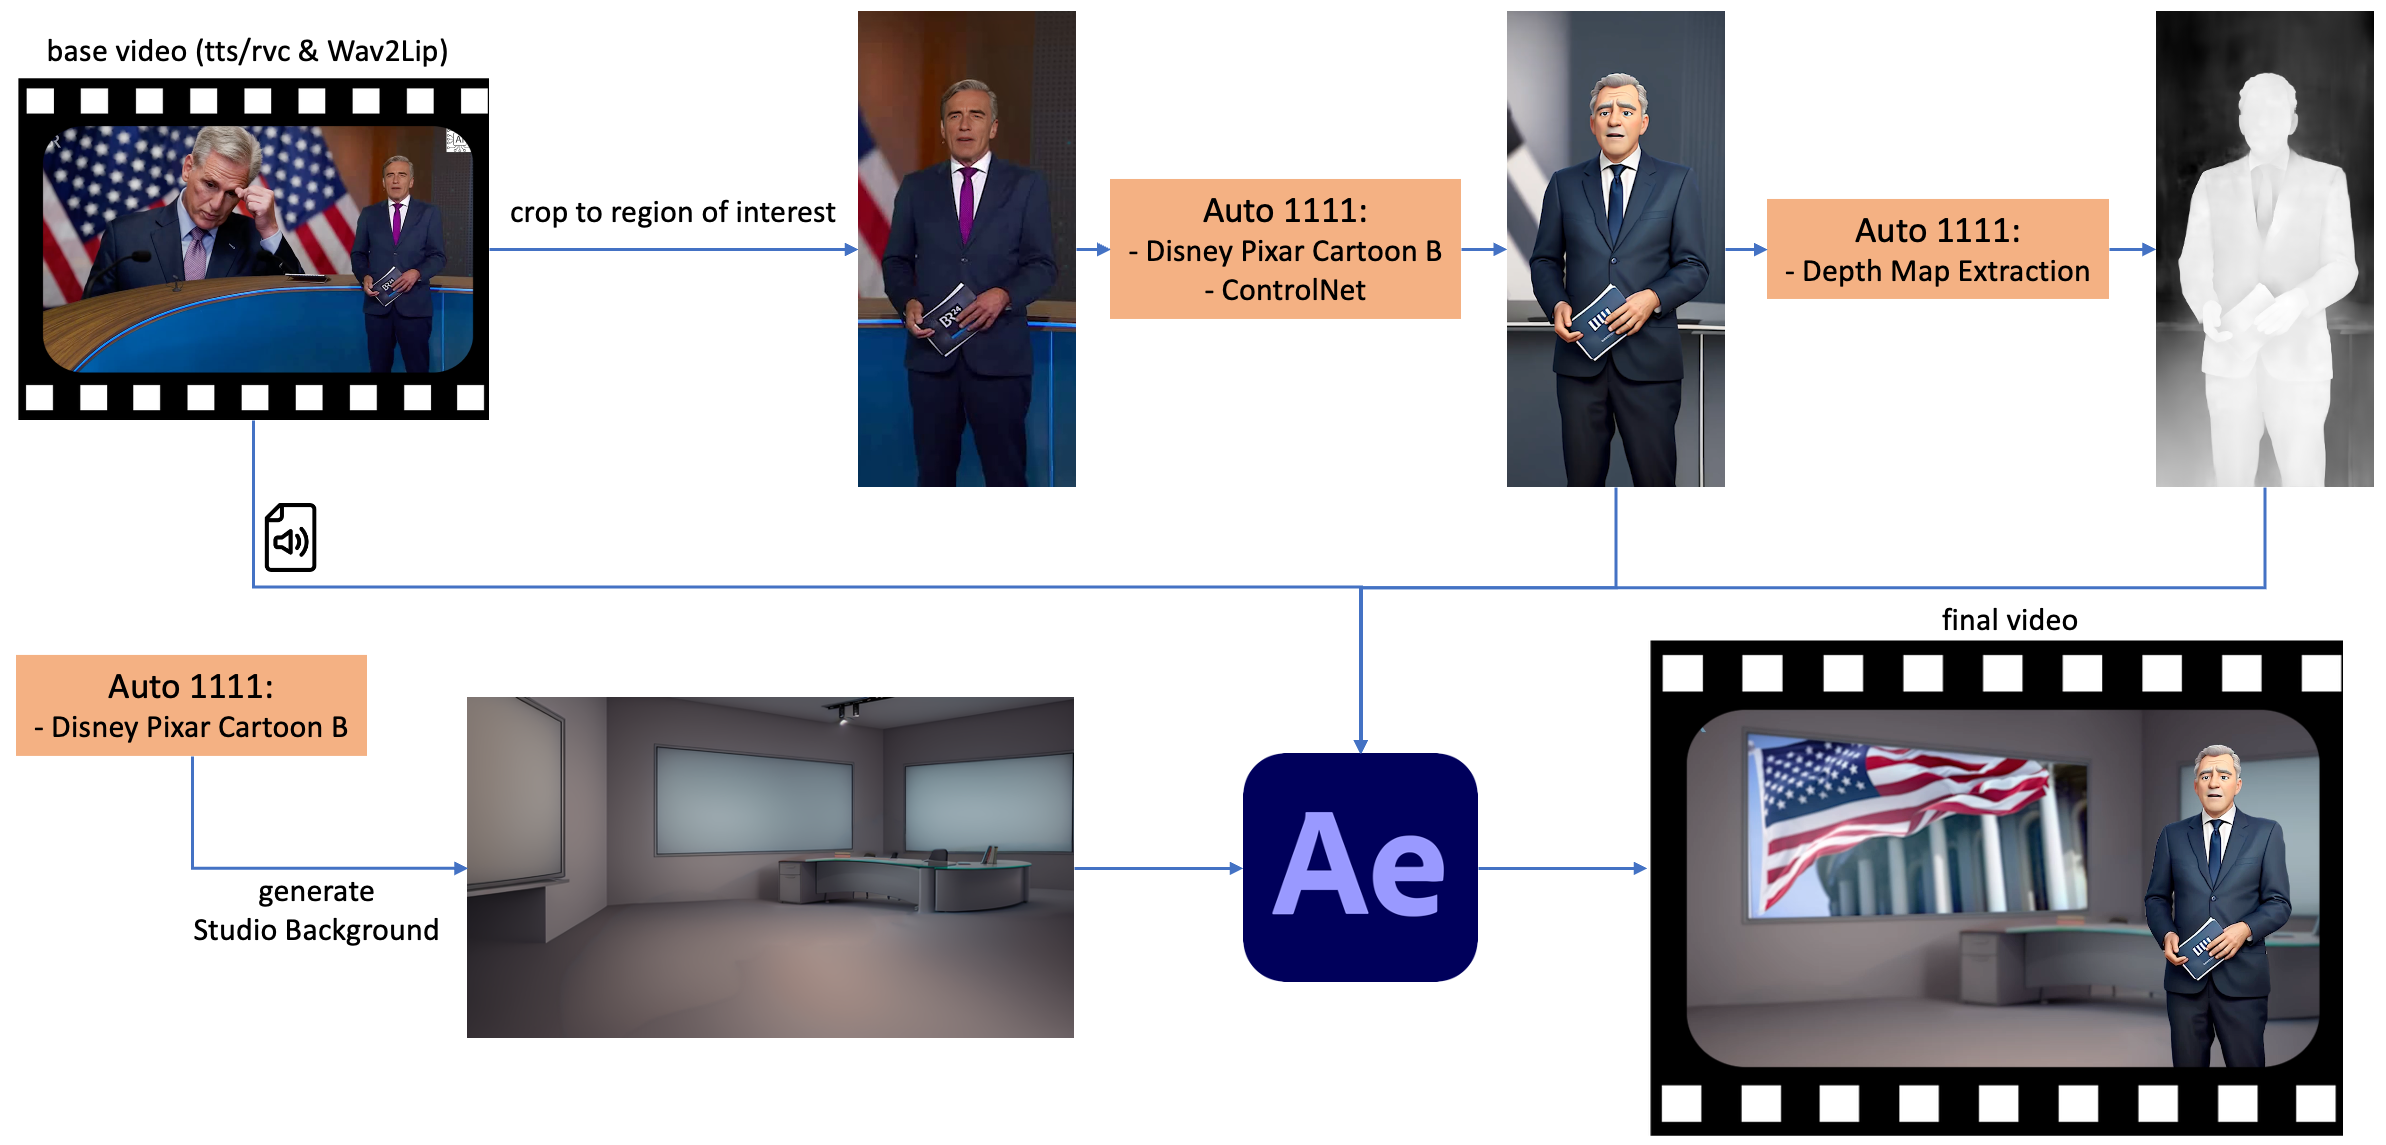
\includegraphics[width=1\textwidth]{./graphics/images/diffusion/sd-workflow.png}
  \caption{Our Stable Diffusion video workflow}
  \label{fig:sd-full-workflow}
\end{figure}

At the time of writing we can report that the ControlNet workflow might already be outdated. In July of 2023 \textit{Animate Diff} was released and offers an alternative workflow to ControlNet. During the making of our experiments Animate Diff was not tested and documented good enough so we could not test it in a reasonable timeframe but it seems in some cases to deliver much better results that ControlNet in both dimensions, control \textit{and} consistency. In November of 2023 Stability AI also released the first Stable Video Diffusion foundation model and shows to have a lot of future potential. 

\subsection{Game-Engine: Unreal Engine}
For the extreme end of our artificiality spectrum (figure \ref{fig:spectrum}) we decided to repurpose an existing project conducted in Unreal Engine. It was part of a master practical at LMU during the summer semester of 2023 under the supervision of Prof. Dr. Johanna Pirker. A detailed report of the practical is available as well, but we will include the most important finding in the following section. \\
The goal of the practical was to glimpse into the possibilities of virtual production, learning basic 3D modelling and the operation of \gls{ue} and accompanying software. To give the goal a concrete example, we wanted to recreate a news show from \gls{br} television which made it an ideal candidate for this paper as well. \\
Although it is quite easy to get started with \gls{ue}, realising complex projects is a difficult untertaking. The main reason lies in the fact that \gls{ue}'s main purpose is aggregating many different assets and giving them logic. Surely it is possible to model, rig and animate characters within \gls{ue} but there are various specialised tools for all of the named tasks: maya, zbrush, blender, iClone Character creator, to just name a few. Doing all of these things is certainly possible in \gls{ue} but has its limits. \\
Mastering many tools takes a lot of time which is why we focussed only on the integrated tools of \gls{ue}. It is quite impressive what can be done with only \gls{ue} in approximately 200 hours of work, but it is also clearly visible that there is a lot of room for improvement. \\
The generated results have neither to do with \gls{genai} nor do they look particularly impressive, probably mostly because the Character is quite uncanny. Still we decided to employ the technology for our paper as well as virtual production is expected to play a huge role in the coming year in regards of synthetic media. In our case we used the renderings as a negative control group for our study. We expected the uncanny avatar to produce the worst credibility due to the uncanny valley effect. A hypothesis we could confirm. For further details please refer to chapter \ref{chap:study}. \\ 
\todo{add data to support hypothesis}
Because of its relevance to synthetic media we decided the include a thorough documentation of the unreal workflow.

\subsubsection*{Unreal Engine Basics}
Before we could start building anything specific, we had to learn some basics of \gls{ue}. There are plenty of free tutorials available online so we first followed. As can be seen from figure \ref{fig:ue-basic-tutorial} the results can look quite impressive after a few hours of learning. This hast to do with \gls{ue}'s excellent library of high quality meshes (3D objects) and easy lighting system. However things look very differently as soon as one tries to create own meshes, textures or characters. 

\begin{figure}[h]
  \centering
  \begin{subfigure}{0.45\textwidth}
    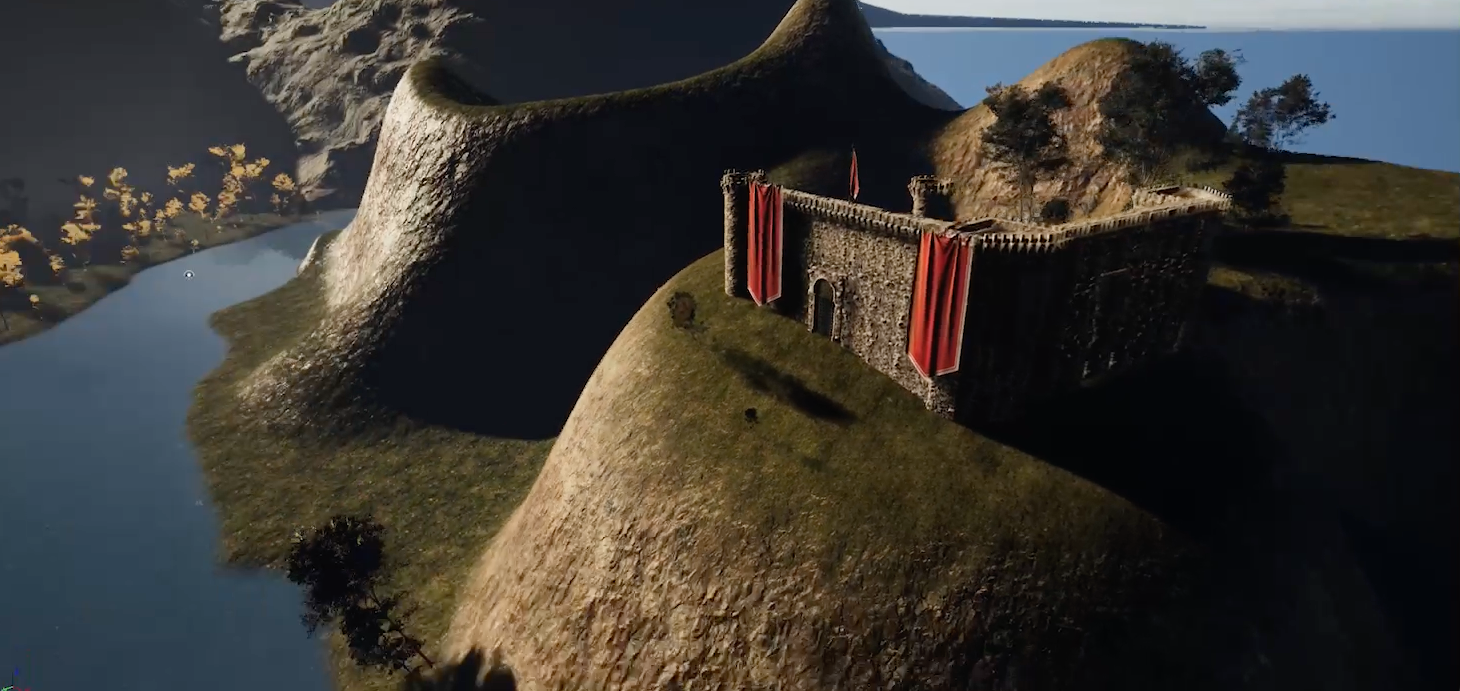
\includegraphics[width=\linewidth]{graphics/images/unreal-engine/Basics/Landscape-Castle.png}
    \caption{Tutorial result: castle}
  \end{subfigure}
  \begin{subfigure}{0.45\textwidth}
    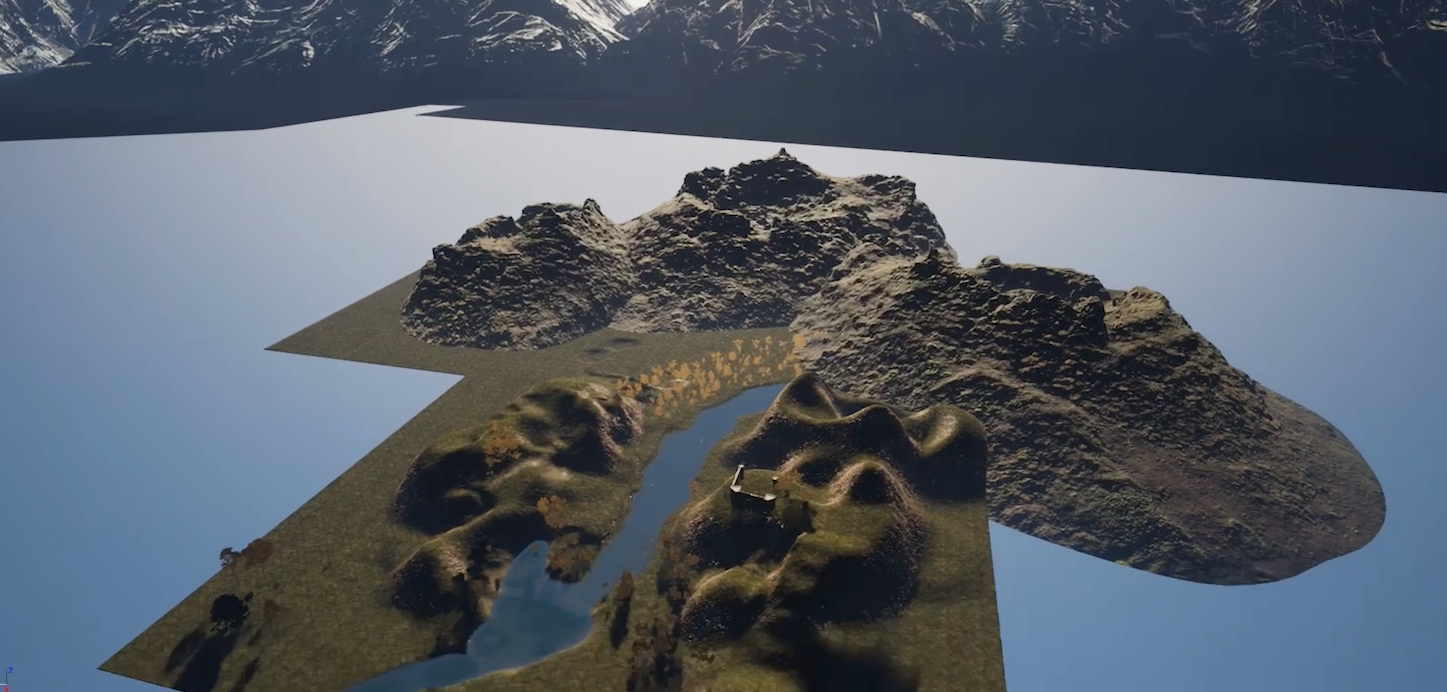
\includegraphics[width=\linewidth]{graphics/images/unreal-engine/Basics/Landscape-Overview.png}
    \caption{Tutorial result: landscape}
  \end{subfigure}

  \begin{subfigure}{0.45\textwidth}
    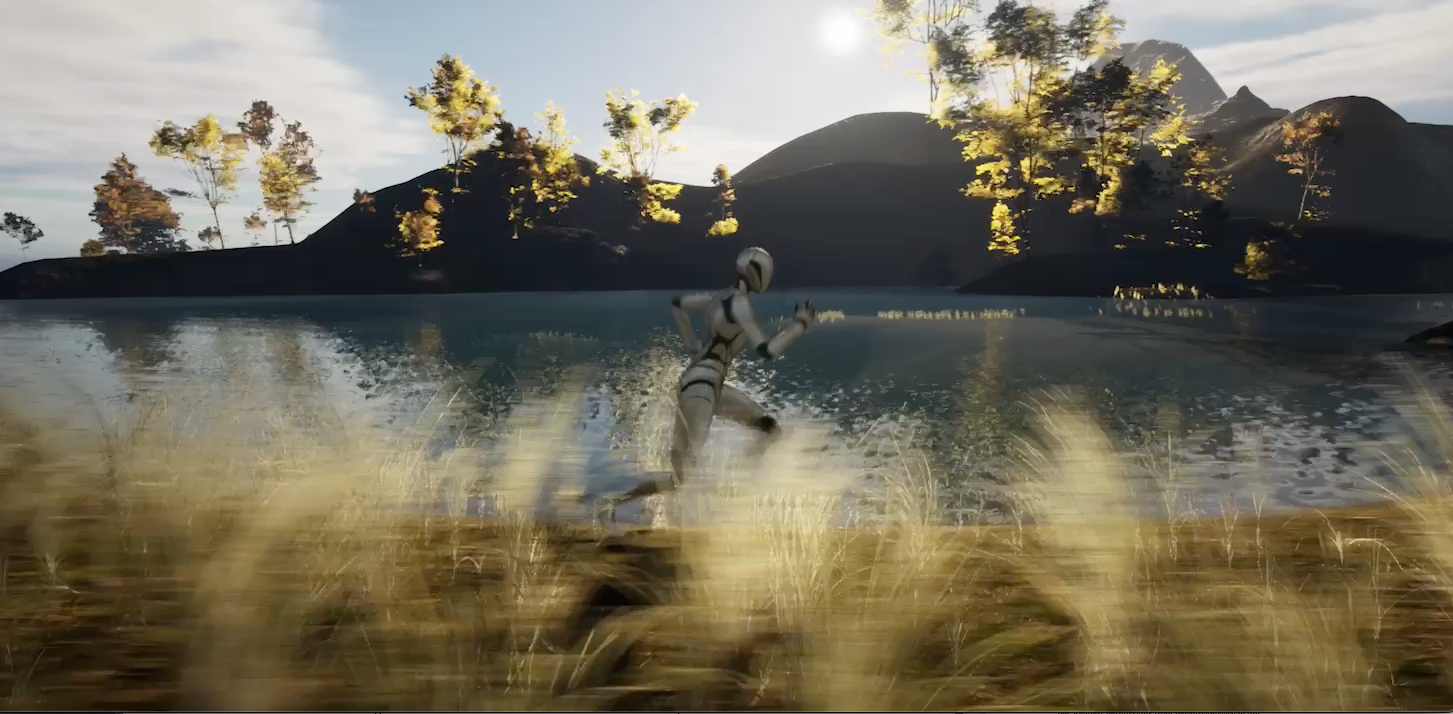
\includegraphics[width=\linewidth]{graphics/images/unreal-engine/Basics/Landscape-running.png}
    \caption{Tutorial result: character running}
  \end{subfigure}
  \begin{subfigure}{0.45\textwidth}
    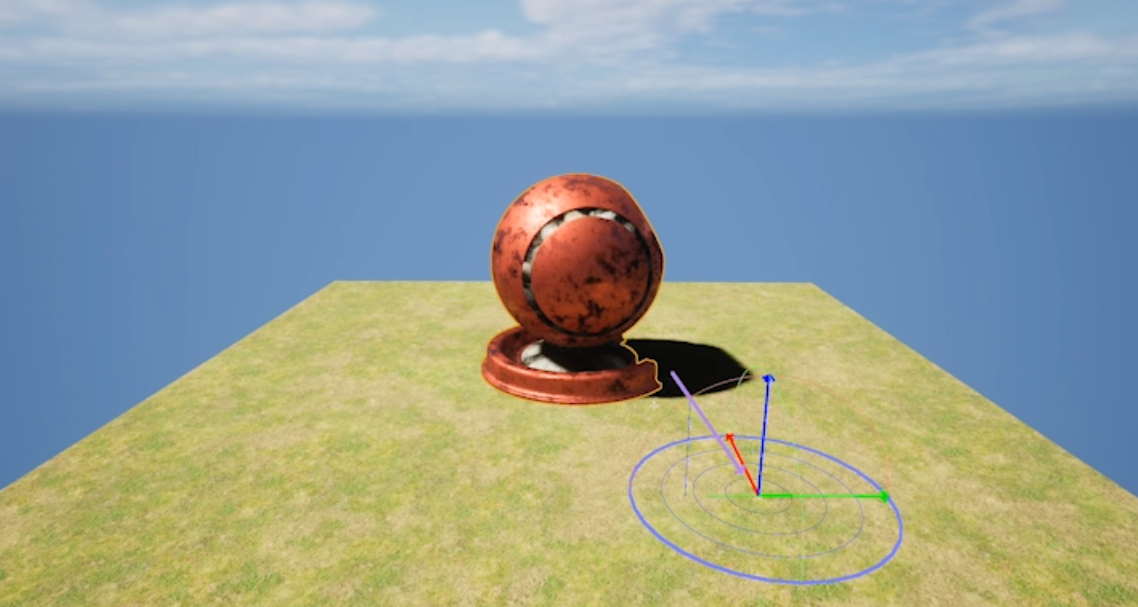
\includegraphics[width=\linewidth]{graphics/images/unreal-engine/Basics/Texture.png}
    \caption{Tutorial result: basic texture}
  \end{subfigure}
  \caption{Results from first tutorial}
  \label{fig:ue-basic-tutorial}
\end{figure}

\subsubsection*{Studio Build}
As we've just mentioned, modeling and texturing are extensive topics on their own. \gls{ue} excels at utilizing and rendering a wide range of objects, including a vast library of assets that can be used for free. Many of these assets are even scanned, providing incredible realism. However, when it comes to modeling custom objects like the studio itself, achieving realism becomes much more challenging. Professional 3D artists would be required to achieve the desired level of accuracy and detail at this point. Nonetheless, it was fascinating to learn the possibilities that Unreal Engine offers even when relying solely on the engine itself. \\
We built the studio with very few elements (see figure \ref{fig:ue-studio-build}). A shiny white floor for reflective lighting, a semicircle backdrop, the main anchorman desk and some generic studio lights at the ceiling. Due to our lacking knowledge about modelling and texturing it does not look very realistic but the similarities to the real counterpart are clearly visible. We tried to at least create a realistic replica of the main desk using photogrammetry (figure \ref{fig:photogrammetry-desk}), but it did not work as expected due to the semi-transparent parts. As an alternative to photogrammetry it would have been interesting to explore how \gls{nerf} or gaussian splatting would have performed in this domain but due to time constrains couldn't be tested during the practical. \\ 
It is to be mentioned that \gls{genai} is becoming very useful in these domains as \gls{sd} is already capable of creating 3D objects with ease. That way modelling and texturing will very likely become much more accessable to semi-professional and amateur users.

\begin{figure}[h]
  \centering
  \begin{subfigure}{0.45\textwidth}
    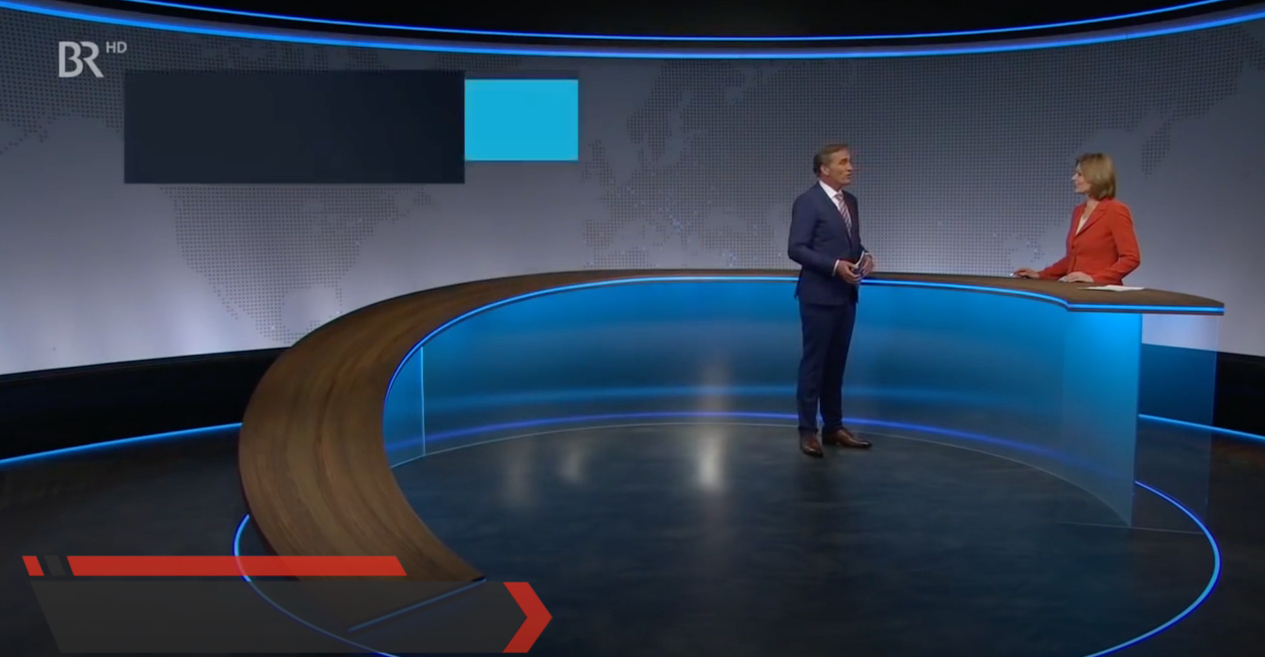
\includegraphics[width=\linewidth]{graphics/images/unreal-engine/studio/Studio-real.png}
    \caption{Real Studio for comparison}
  \end{subfigure}
  \begin{subfigure}{0.45\textwidth}
    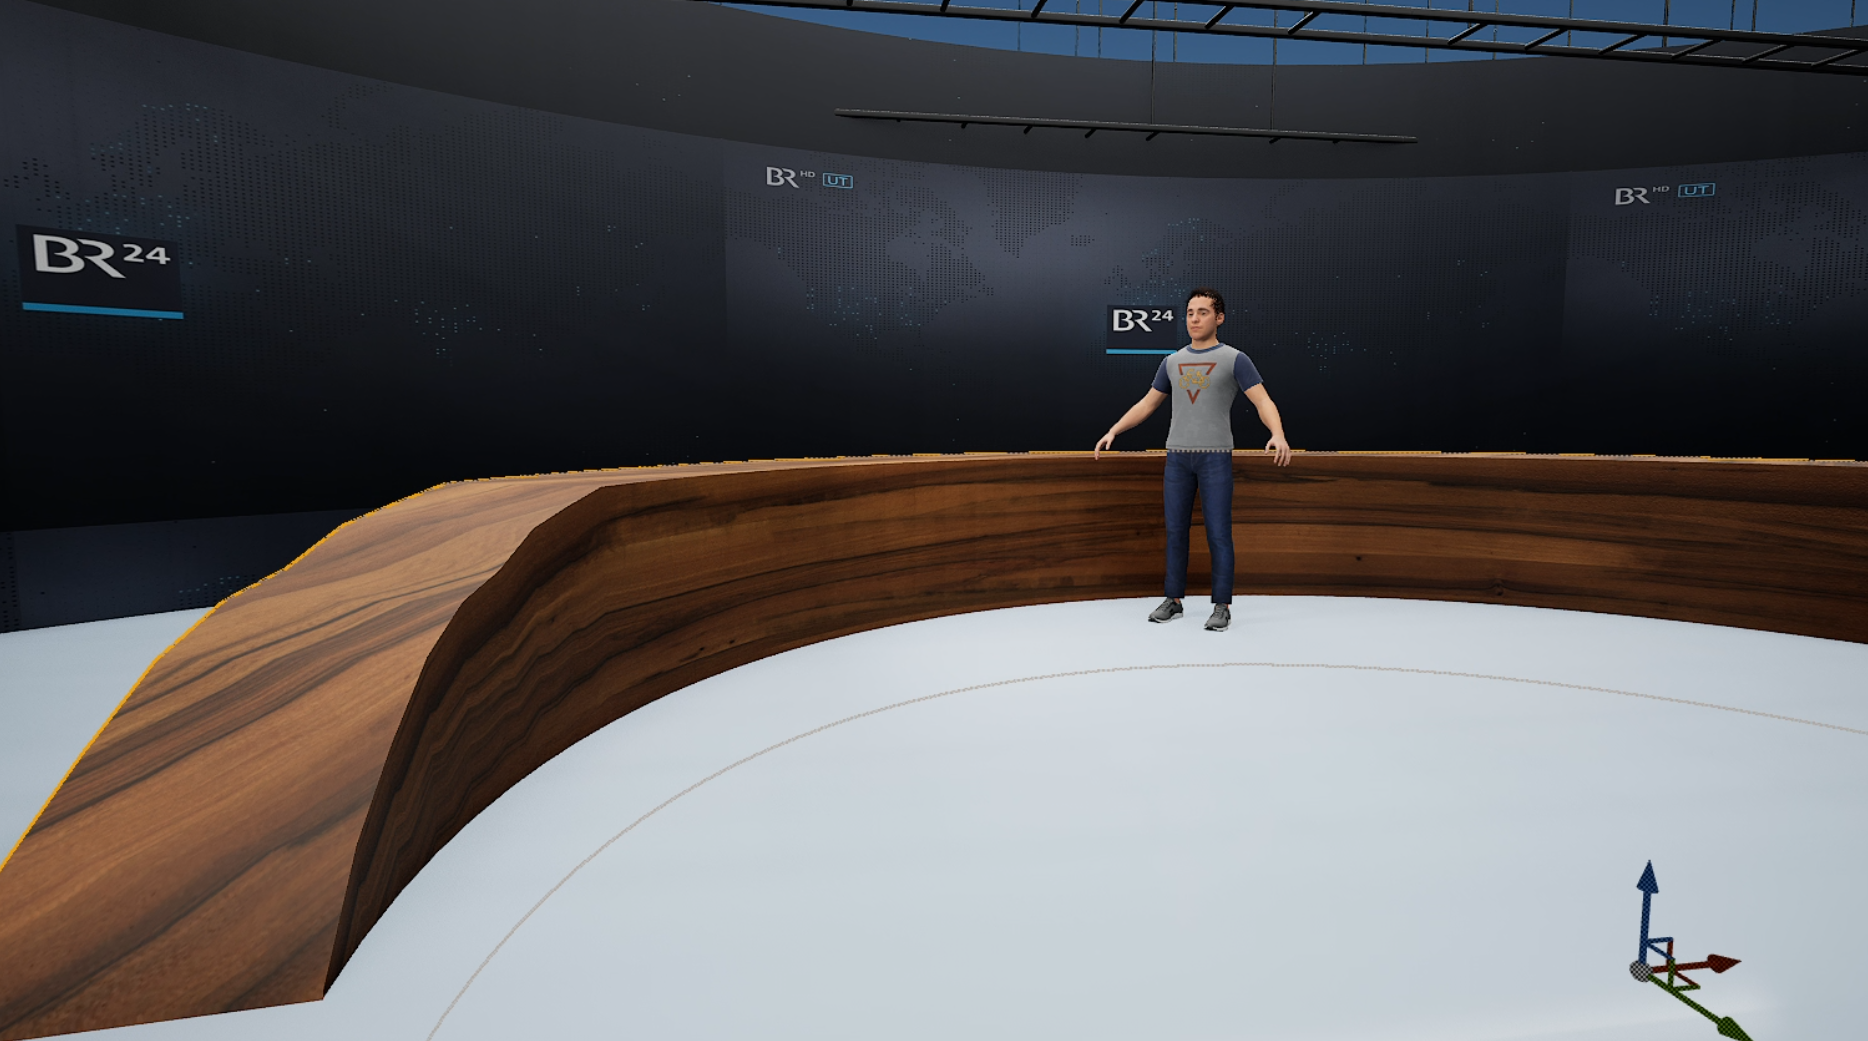
\includegraphics[width=\linewidth]{graphics/images/unreal-engine/studio/Studio-Comparison.png}
    \caption{Studio recreation modelled in \gls{ue}}
  \end{subfigure}

  \begin{subfigure}{0.45\textwidth}
    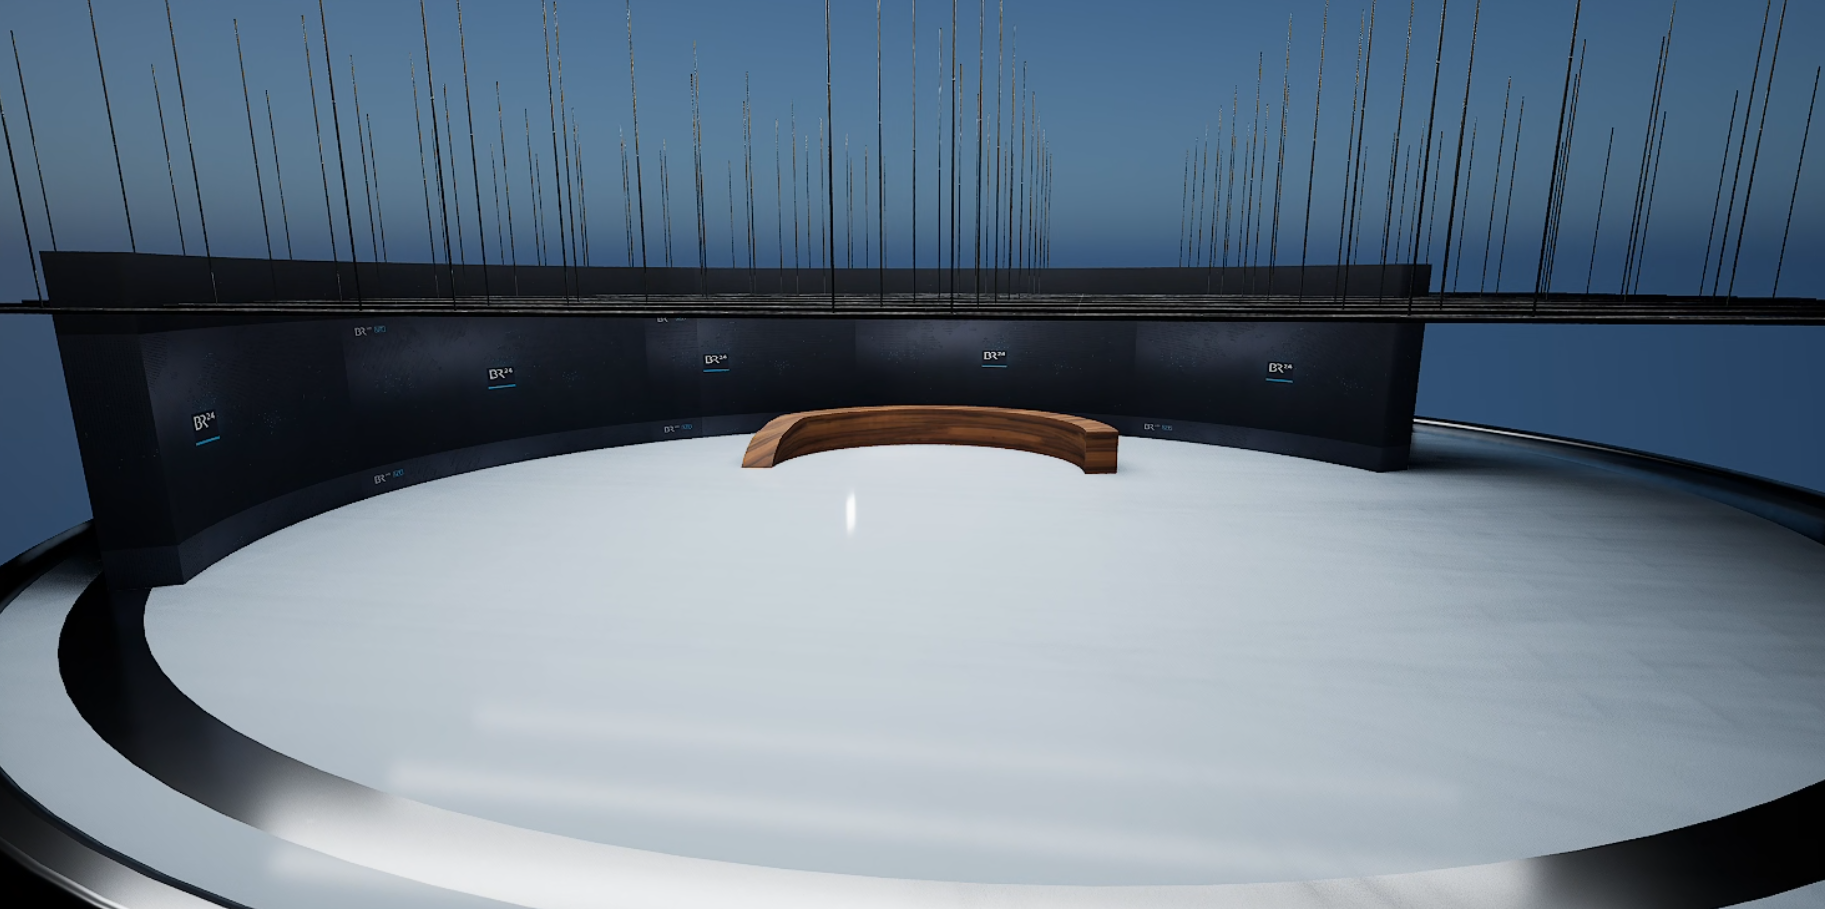
\includegraphics[width=\linewidth]{graphics/images/unreal-engine/studio/studio-totale.png}
    \caption{Studio lighting}
  \end{subfigure}
  \begin{subfigure}{0.45\textwidth}
    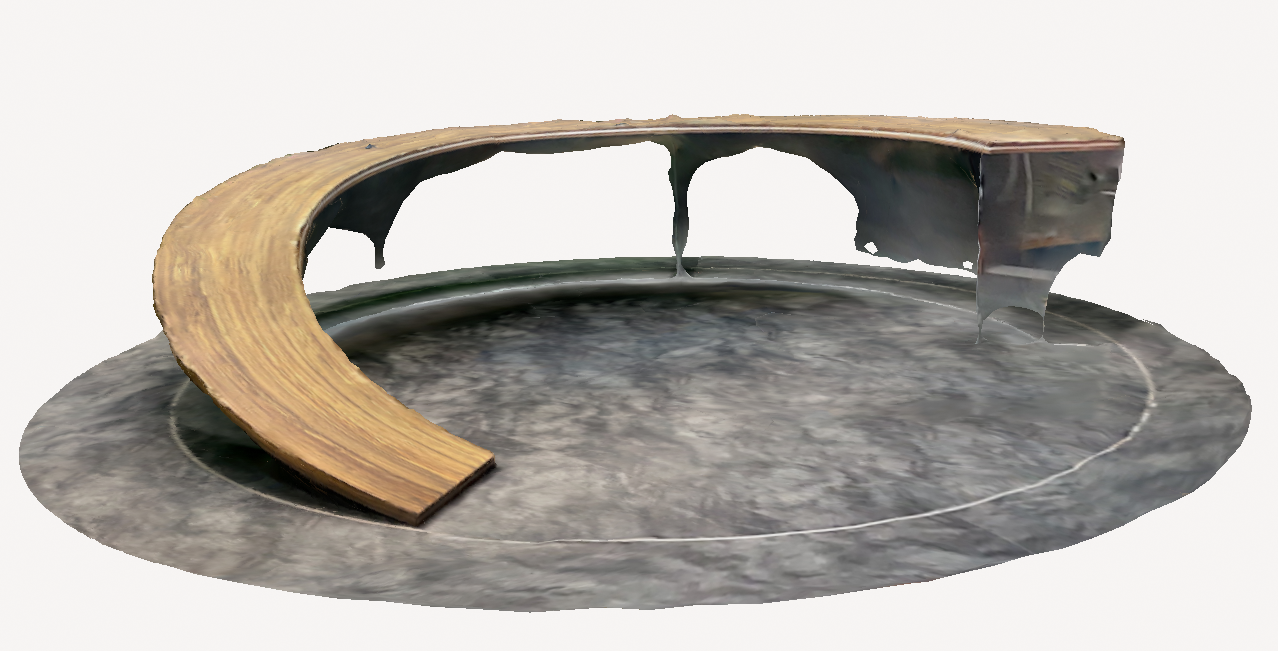
\includegraphics[width=\linewidth]{graphics/images/unreal-engine/studio/Photogrammetry-Desk.png}
    \caption{Experiment: photogrammetry scan of main desk}
    \label{fig:photogrammetry-desk}
  \end{subfigure}

  \caption{Unreal Engine TV Studio Build}
  \label{fig:ue-studio-build}
\end{figure}

\subsubsection*{Camera and Media Playback Logic} 
With the studio in place, a camera system needed to be implemented. \gls{ue} already provides support for \textit{cine-cameras}, which offer various settings reminiscent of their real-world counterparts, such as aperture, exposure, focal length, and focus. Initially, transitioning between cameras seemed straightforward using the integrated \textit{set view Target with blend} method. It was easy to set up multiple cameras within the scene and cut or animate between them using the mentioned method. This approach resembled the camera robots used in the real studio, utilizing easy-ease keyframes, which was advantageous. \\
However, there was a significant limitation with the existing method. While it effectively moved and rotated the view to the desired position, other parameters such as focal length, focus distance, and aperture did not change until the transition was complete. As a result, after the transition, these settings abruptly shifted, creating an undesirable visual effect. This behavior was unacceptable when aiming for smooth transitions. \\
To fix these issues it was necessary to develop a seperate camera system with custom control over the animation using \gls{ue}'s visual scripting language \textit{blueprint}. The scene now includes a Master-Camera controlled by a blueprint script \ref{fig:blueprint}. This blueprint inherits methods for updating all relevant camera parameters, including a transition time that can be passed into the function call.
\begin{figure}[h]
  \centering
  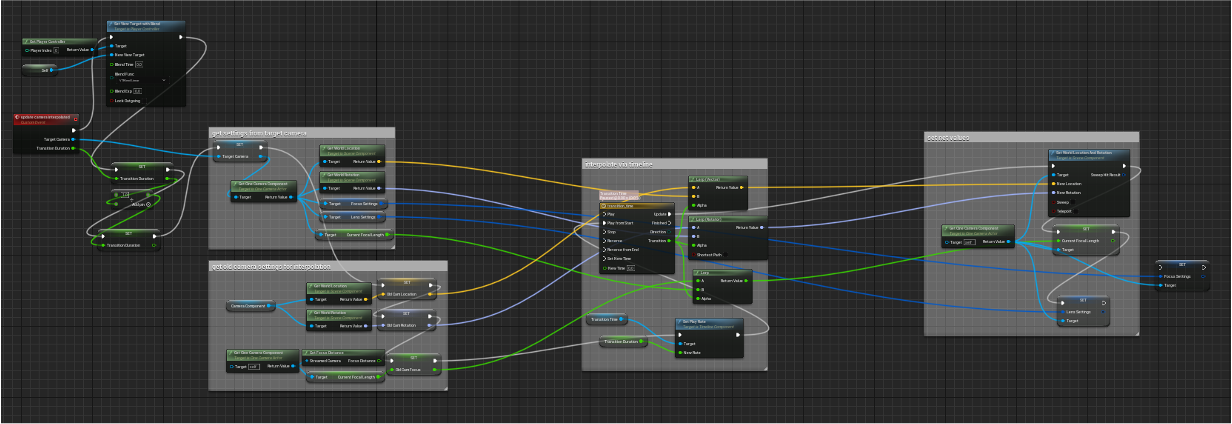
\includegraphics[width=1\textwidth]{graphics/images/unreal-engine/blueprint.png}
  \caption{Camera Blueprint}
  \label{fig:blueprint}
\end{figure}
With the custom camera system in place, an endless number of cameras can be set up and animated between, which proves to be quite useful. Two example cameras are depicted in figure \ref{fig:cameras}.

\begin{figure}[h]
  \centering
  \begin{subfigure}{0.45\textwidth}
    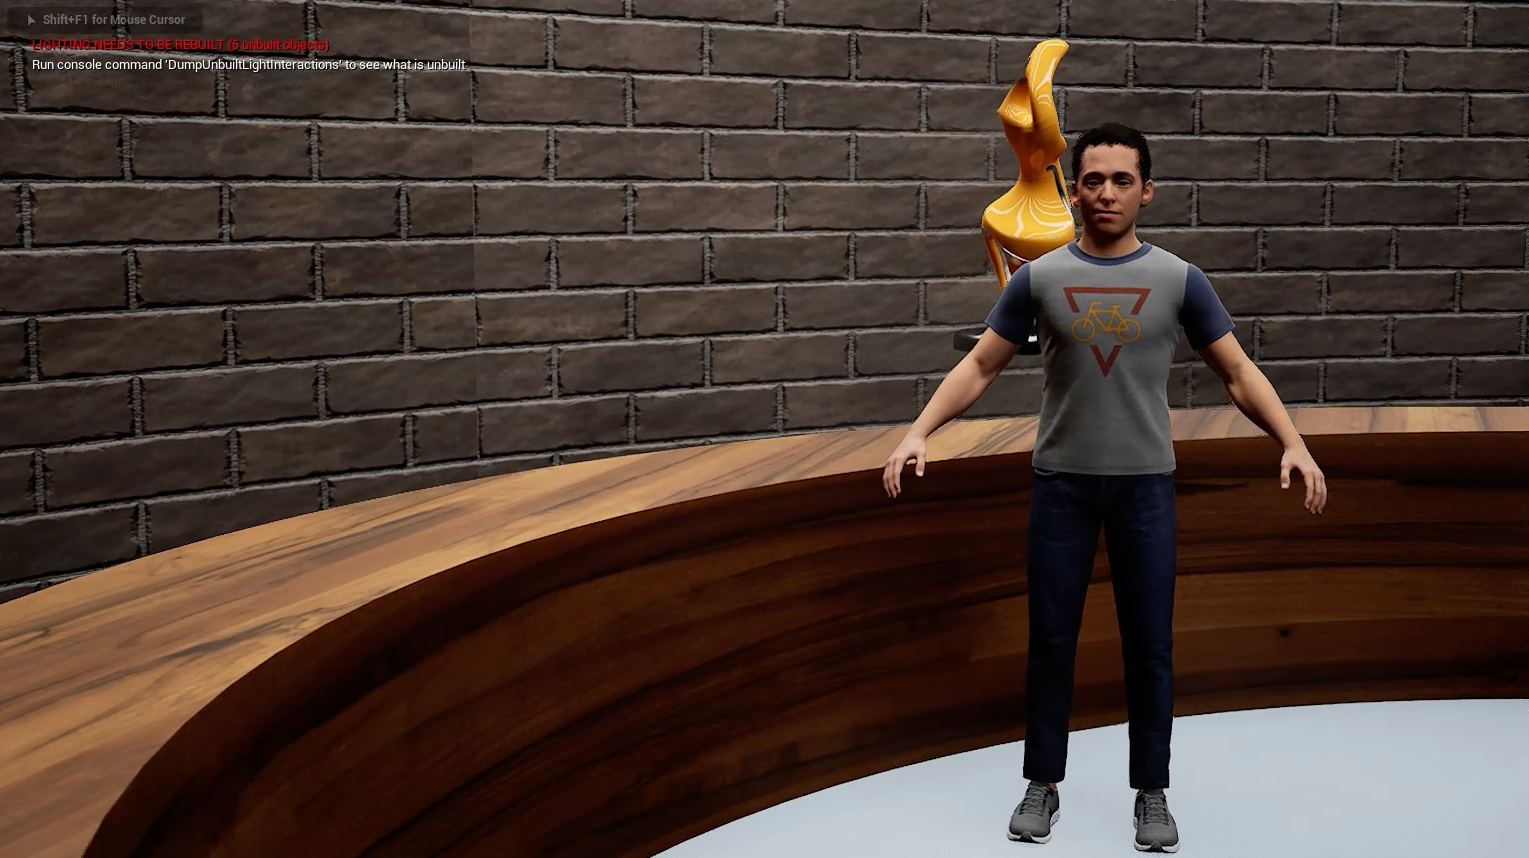
\includegraphics[width=\linewidth]{graphics/images/unreal-engine/camera angles/medium closeup.png}
    \caption{medium shot}
  \end{subfigure}
  \begin{subfigure}{0.45\textwidth}
    \includegraphics[width=\linewidth]{graphics/images/unreal-engine/camera angles/close up.png}
    \caption{medium close-up}
  \end{subfigure}
  \caption{two virtual camera examples in the studio}
  \label{fig:cameras}
\end{figure}

In many news formats, graphics presentations play a significant role. Analogously to the camera logic we had to implement a blueprint for the media playback in the background of the anchorman (see figure \ref{fig:ue-media}). These presentations can be implemented in various ways, such as changing the background image or displaying a floating image next to the host. To better understand how BR24 accomplishes this, we spent time with video engineers on the show. The complexity of their system was overwhelming: BR24 has hundreds of templates for how hosts can present content, all rendered in real-time using a \textit{viz.rt} graphics engine. \\
To keep the practical within a manageable scope, we decided to implement only one mockup display behind the news host, as depicted in Figure \ref{fig:ue-media}. The technical implementation of this feature is well-documented in \gls{ue} tutorials. It involves using a \textit{media-player} feature that renders a material onto a plane mesh.
We've briefly considered using separate software like \gls{obs} to render graphics, but opted against it. Introducing another piece of software would have added complexity and reduced customizability. It would have also run against the idea of doing as much as possible inside UE. \\
Similar to the camera system, additional functionality had to be added to the projection plane to use it in the desired manner. This was achieved by leveraging the knowledge gained from developing the camera system. Custom blueprints were created to control the behavior of the projection plane and expose callable methods. This enabled control over parameters such as opacity, fade-in/fade-out effects, loading and changing display images during runtime, and playing and pausing video media. \\
However, one issue remained with the projection plane: the images are not yet standardized, resulting in distortion. This will need to be addressed by applying appropriate adjustments to ensure the images appear undistorted. Additionally, camera positions need to be set to ensure the content in the background aligns appropriately with the projection.

\begin{figure}[h]
  \centering
  \begin{subfigure}{0.45\textwidth}
    \includegraphics[width=\linewidth]{graphics/images/unreal-engine/media/slide-real.png}
    \caption{real media panel reference}
  \end{subfigure}
  \begin{subfigure}{0.45\textwidth}
    \includegraphics[width=\linewidth]{graphics/images/unreal-engine/media/slide-inplace.png}
    \caption{media panel visible}
  \end{subfigure}
  \caption{virtual media display}
  \label{fig:ue-media}
\end{figure}

\subsubsection*{Character Build}
\gls{ue} provides its own toolset for creating comprehensive virtual characters, so called \textit{Metahumans}, which facilitates character creation to some extent. Like \gls{ue}, the Metahuman editor facilitates quick results but has limitations to modeling and texturing—customization options. To mitigate this problem, specialized software such as \textit{iClone Character Creator} or 3D animation software like \textit{Maya} or \textit{Blender} could be utilized. During the practical these alternatives could not be covered, which is why we relied solely on \gls{ue}'s Metahuman editor. \\
Metahumans are currently undergoing active development and evolving rapidly. Editing Metahumans is done through a cloud rendering web application in the browser, which is then synced to \gls{ue}. Creating a new character can be done from scratch or based on a real human, however, the method to achieve this changed over the course of several weeks, which shows the pace of development. In December of 2023 \textit{gaussian avatar} are available in first, experimental implementation. This will drastically improve future workflows. \\
For our case, we initially had to employ a workflow called "mesh to metahuman", which required a 3D mesh of a head to be imported into \gls{ue}. From there, it could be converted into a Metahuman. We captured a head scan using the same photogrammetry workflow as with the studio table. The scan yielded exceptional results, as depicted in figure \ref{fig:head-photogrammetry-scan}. \\
Unfortunately, the resulting Metahuman character did not bear much resemblance to the scan, as shown in Figure \ref{fig:metahuman-result}. With more expertise in character modeling, it may be possible to improve the likeness to a large extent. \\
During our research, \gls{ue} version 5.2 was released, introducing a new workflow that utilizes the faceID lidar sensors of an iPhone to capture facial performance data. The results were much better than the "mesh to metahuman" workflow. Still, the Metahuman character creator lacks customization options in various aspects, hindering us to achieve higher likeness.

\subsubsection*{Character Animation}

Next we needed to bring the character to life through animation. There were several options for achieving that objective, including using prerecorded performance data or implementing a live capture workflow. For the news format, a responsive and quick-to-produce approach was desirable, making the live version preferable. However, implementing a full live capture system would require extensive tracking hardware, such as a full-body tracking suit. These suits can range in cost from 2.000€ to 5.000€ and can be complex to calibrate. Given the time constraints, a simpler and more cost-effective solution was chosen for the prototype. \\
Firstly, facial tracking using the iPhone's FaceID sensors. This allows for tracking of facial expressions and head rotation. Unreal Engine provides easy support for this, requiring only an iPhone on the same network as the Unreal PC and sometimes necessitating custom firewall settings. One challenge, however, is directing the gaze of the eyes towards a virtual camera. If the eyes do not look into the camera, the character can appear uncanny.
\begin{figure}[h]
  \centering
  \includegraphics[width=0.5\textwidth]{graphics/images/unreal-engine/MH/bent-head.png}
  \caption{Uncanny results from our animated metahuman}
  \label{fig:uncanny mh}
\end{figure}
Secondly, the rest of the body received an idle animation in the form of simple breathing. That way the body looked more natural while the face was driven by an actor recording the moderation using the iPhone FaceID sensor. The end result has a lot of room for improvement. Especially the face animations look quite uncanny (see figure \ref{fig:uncanny mh}). The eyes don't focus the camera and only few facial landmarks are animated. This has to do with technical limitations of the facial capture as there are too few facial landmarks being tracked. \\
All in all the performance falls deep into the uncanny valley making it the perfect example for our negative control group. 


\newpage
\section{Study}
\label{chap:study}
During our research and work in the film and television industry we have encountered various anecdotal assessments about trust towards synthetic media. In regards to the scarce research landscape in such a young topic we decided to conduct our own exploratory study in the area of synthetic media trust and credibility. \\
As there are many different methods of creating synthetic media, we wanted to test them against each other and see how they perform. This resulted in our main research question (RQ1) of how the artificiality of synthetic media influences trustworthines. Other questions in neighbouring fields were postulated along the way (refer to \ref{tab:research-questions}).

\begin{table}[h]
  \centering
  \begin{tabularx}{\textwidth}{l|X}
    \textbf{Research Question/Hypothesis} & \textbf{Description}\\
    \midrule
    RQ1a & Will video artificiality have an impact of trustworthines?  \\
    \midrule
    RQ1b & Does age, education or profession impact the effects in RQ1a?  \\
    \midrule
    RQ1c & What effect does the screen size have on the effects in RQ1a?  \\
    \midrule
    RQ2a & What effect does an "AI Logo" label have?\\
    \midrule
    RQ2b & Does age, education or profession impact the effects in RQ2?  \\
    \midrule
    RQ2c & What effect does the screen size have on the effects in RQ2?  \\
  \end{tabularx}
  \caption{Research Questions and Hypothises}
  \label{tab:research-questions}
\end{table}

\subsection{Study Design}
\label{subsec:study design}

Our goal was to find out more about the relationship of various types of synthetic media and their trustworthines. In chapter \ref{chap:background} we have treated the relevant technologies we have aquired over the time. With access to these tools we wanted to design a study that utilizes them in a practical scenario which is close to a daily practice use case. We therefore chose the TV newscast as a good testing environment. It provided sufficient control, yet the ability to experiment with \gls{tts}, \gls{v2v}, \gls{sd} or even \gls{ue}. \\
The newscast set the content. We chose to build upon existing news and not invent any to keep them realistic. This should have eliminated bias towards unrealistic news, but unfortunately we did not take into account differing knowledge. We will address this issue later while discussing the limitations of our study. \\
We decided to craft our study around the aforementioned spectrum of artificiality as depicted in figure \ref{fig:spectrum}. By introducing an increasing amount of synthetic media at each stage, we were hoping to measure effects on trust. The artificiality therefore was one of our most important independent variables. The artificiality has close ties to the uncanny valley effect. Using several questions, we calculated a perceived index for each video. To avoid ambiguity with the term AI, we will name this index \gls{ri} instead of "artificiality Index". High /gls{ri} is analogous to low artificiality and a low uncanny valley effect.\\
We anticipated that the content itself would also have some effect on the judgements. To mitigate these issues we created a second video at each quality level but filled it with different content. That way we were able to controle and compare results in both content groups. \\
Discussions about \gls{genai} lead quickly to the call of marking footage, that has been created with AI. We wanted to address this topic and decided to test for this as well. We did this by placing an AI logo in the upper corner of half of the videos. The meaning of the AI logo was explained in advance. To be ethically correct we informed the participants that the AI Logo marks AI generated content in some cases, but can also be wrongly marked in other cases. While our study was already running, we discovered the paper by \citeauthor{toffTheyCouldJust2023}, where the authors conducted similar testing in the domain of AI generated texts. Unfortunately we couldn't incorporate their findings to optimize our study design. But since the AI mark test was just an add-on to our main research question this wasn't too much of a missed opportunity. Please refer to table \ref{tab:video-table} for a clear overview about the artificiality level, content and AI Logo marking strategy.


\begin{table}[h]
  \centering
  \begin{tabularx}{\linewidth}{c|c|X|X}
    
    \textbf{ID} & \textbf{AI Logo} & \textbf{Content} & \textbf{Artificiality}\\
    \midrule
    1\_1 & in group B & German unification day celebrations  & None: real video from broadcast \\
    \midrule
    1\_2 & in group A & USA, McCarthy impeachment  & None: real video from broadcast \\
    \midrule
    2\_1 & in group B & Smartphone usage decreased at Oktoberfest  & audio generated with \gls{v2v} conversion, video real+\gls{w2l} \\
    \midrule
    2\_2 & in group A & Introduction of new traffic management system  & audio generated with \gls{v2v} conversion, video real+\gls{w2l} \\
    \midrule
    3\_1 & in group B & Youth music festival in bavaria  & audio generated with \gls{tts}, video real + \gls{w2l} + style transformation with \gls{sd} \\
    \midrule
    3\_2 & in group A & US democratic party under pressure  & audio generated with \gls{tts}, video real + \gls{w2l} + style transformation with \gls{sd} \\
    \midrule
    4\_1 & in group B & Robert Habeck visits Gamescom  & audio generated with \gls{v2v} conversion, video filmed in \gls{ue} \\
    \midrule
    4\_2 & in Group A & Biden visits middle east  & audio generated with \gls{v2v} conversion, video filmed in \gls{ue} \\
  \end{tabularx}
  \caption{Description of our test videos}
  \label{tab:video-table}
\end{table}

Finally we needed to layout our test videos in a specific way to avoid side effect measurings by the content of the videos, the order of the videos (sequence bias) and the AI marking of the videos (see table \ref{tab:video-table}): \\
In total there were eight videos, two for each of the four artificiality stages. In Group A, the second video within an artificiality stage was marked by the AI Logo. Group B had it reversed, meaning the first video of each stage was marked. \\
During interrogation each participant was randomly assigned to Group A or B. This measure was meant to compensate for side effects created by content variation. The size of the groups was continously balanced so that Groups A and B stayed at similar sizes. \\
Within each group, the participant was the presented to all the eight video one after the other. The order of the videos were randomized for each participant, in order to mitigate sequence bias. All questions in regards to a specific video were answered alongside the concerning video, while no other video was present. This, in addition to the random sequence was meant to reduce direct comparability effects.

In addition to the video questionaire we've asked for basic demographic information. 
Our study encompasses both, a between subject design (A/B Group division) and a within subject design (analysis within Group A or B). However sample size within the groups was probably too small for certain tests.

\subsection{Procedure and Participants}
The study was designed as an online questionaire, conducted via the survey platform "soSci survey", hosted by the University of Munich. The survey was reachable via a single URL. The URL was spread among various media companies, university groups and the author's personal contacts. \\
After following the URL, a visitor was immediatly assigned to group A or group B of the questionaire. It survey itself was divided into 3 stages: 1) general and democraphical questions, 2) main video evaluation, 3) post-questionaire evaluation and study explanations. \\ 
During the second stage, all videos were presented to the participant in a randomized sequence. Along with each video the participant had to answer five questions on a likert scale of \textit{one} to \textit{six}.
\begin{enumerate}
  \item The content of this video is true.
  \item This video seems trustworthy.
  \item The anchorman is real.
  \item The anchroman's voice is real.
  \item The video has a good quality.
\end{enumerate}
In addition to the likert scale the participants also had the opportunity to answer any of the questions with additional free text remarks. \\
During the post-questionaire we questioned how focussed the participants were during the survey and how serious they listened to the videos. On a scale of \textit{one} ot \textit{three} we received a meaninglessnes mean of 1.138 (closer to 1 is better) and distraction of mean of 1.318 (closer to 1 is better). On a four steps scale of how much the participants enjoyed the study (from \textit{not at all} to \textit{very much}) we received a mean of 3.185 (closer to 4 is better). According to these values we infer that our gathered data accurately represents our participants meaning and isn't skewed by their unwillingnes to participate. \\
After all questions were answered, we provided an explainatory video for the study with a call to further spread the survey among friends and colleagues. We further incentivised participants to take part in the study by offering 50€ to be given away in a lottery after the study has been finished.

In total we could gather N=195 valid participants. Regarding the age distribution the median lies at 30-34 (see \ref{fig:age-distribution}).
\begin{figure}[h]
  \centering
  \includegraphics[width=1\textwidth]{graphics/images/statistics/age-plot.png}
  \caption{sample age distribution}
  \label{fig:age-distribution}
\end{figure}
The distribution of industrial sectors show a focus on IT (24.6\%) and creative media (39.5\%) (table \ref{tab:frequenciesForBranch}) while most participants were currently employed (50.3\%) or in education (28.2\%) (table \ref{tab:frequenciesForOccupation}). 
\begin{table}[h]
	\centering
	\caption{Frequencies for industrial sector}
	\label{tab:frequenciesForBranch}
	{
		\begin{tabular}{lrrrr}
			\toprule
			Sector & Frequency & Percent & Valid Percent & Cumulative Percent  \\
			\cmidrule[0.4pt]{1-5}
			agriculture & $2$ & $1.026$ & $1.026$ & $1.026$  \\
			production & $6$ & $3.077$ & $3.077$ & $4.103$  \\
			construction & $2$ & $1.026$ & $1.026$ & $5.128$  \\
			trade & $1$ & $0.513$ & $0.513$ & $5.641$  \\
			gastronomy \& tourism & $1$ & $0.513$ & $0.513$ & $6.154$  \\
			transport \& logistics & $3$ & $1.538$ & $1.538$ & $7.692$  \\
			IT & $48$ & $24.615$ & $24.615$ & $32.308$  \\
			finance \& insurance & $6$ & $3.077$ & $3.077$ & $35.385$  \\
			healthcare & $12$ & $6.154$ & $6.154$ & $41.538$  \\
			education & $18$ & $9.231$ & $9.231$ & $50.769$  \\
			government & $9$ & $4.615$ & $4.615$ & $55.385$  \\
			creative & $77$ & $39.487$ & $39.487$ & $94.872$  \\
			environmental & $1$ & $0.513$ & $0.513$ & $95.385$  \\
			other & $9$ & $4.615$ & $4.615$ & $100.000$  \\
			Total & $195$ & $100.000$ & $ $ & $ $  \\
			\bottomrule
		\end{tabular}
	}
\end{table}
\begin{table}[h]
	\centering
	\caption{Frequencies for occupation}
	\label{tab:frequenciesForOccupation}
	{
		\begin{tabular}{lrrrr}
			\toprule
			Occupation & Frequency & Percent & Valid Percent & Cumulative Percent  \\
			\cmidrule[0.4pt]{1-5}
			in school & $1$ & $0.513$ & $0.513$ & $0.513$  \\
			apprentice & $10$ & $5.128$ & $5.128$ & $5.641$  \\
			student & $44$ & $22.564$ & $22.564$ & $28.205$  \\
			employed & $98$ & $50.256$ & $50.256$ & $78.462$  \\
			civil servant & $11$ & $5.641$ & $5.641$ & $84.103$  \\
			self employed & $26$ & $13.333$ & $13.333$ & $97.436$  \\
			unemployed & $2$ & $1.026$ & $1.026$ & $98.462$  \\
			pensioner & $3$ & $1.538$ & $1.538$ & $100.000$  \\
			Total & $195$ & $100.000$ & $ $ & $ $  \\
			\bottomrule
		\end{tabular}
	}
\end{table}
We have also collected data about last educational institution graduated, gender and country but these factors had no relevant effects and thus can be ommitted. \\
In regard of the uses display device the smartphone, laptop monitors and larger external monitors were quite evenly distributed (compare table \ref{tab:frequenciesForDevice}). We will compare this self assessment with our measurements later on.
\begin{table}[h]
	\centering
	\caption{Frequencies for display device}
	\label{tab:frequenciesForDevice}
	{
		\begin{tabular}{lrrrr}
			\toprule
			Device & Frequency & Percent & Valid Percent & Cumulative Percent  \\
			\cmidrule[0.4pt]{1-5}
			smartphone & $59$ & $30.256$ & $30.256$ & $30.256$  \\
			laptop & $66$ & $33.846$ & $33.846$ & $64.103$  \\
			external monitor & $70$ & $35.897$ & $35.897$ & $100.000$  \\
			\bottomrule
		\end{tabular}
	}
\end{table}
Lastly, we asked participants which of the the factors (video content, video quality or AI-Logo) had the strongest influence to their judgments in regards of the perceived trustworthiness (see figure \ref{fig:most-influence}).
\begin{figure}[h]
  \centering
  \includegraphics[width=.5\textwidth]{graphics/images/statistics/most-influence.png}
  \caption{sample's judgement about most influential trust factors.}
  \label{fig:most-influence}
\end{figure} 

\subsection{Results}

Before we start with further analysis we wanted to address the topic of handling Likert scales. We are aware of the ongoing discussion about wether Likert scales can produce and be interpreted as metric data or if it can only supply ordinal data. The central argument against is, that equidistance between the options cannot be ensured. Devaluing these scales to ordinal data would prohibit arithmetic operations with the values as well as many statistical tests. Many Likert scales use a scale of four items and there are recommendations to increase the number of Likert scale points to make it closer to continuous scales and normality \cite{wuCanLikertScales2017a}. We complied by using six points, instead of four. In our next research we will most likely use ten or eleven points as suggested by \Citeauthor{hodgePhraseCompletionScales2007}. We further assume our Likert measurements to be metric, however we checked some parametric tests with their non-parametric counterparts to ensure they wouldn't deliver drastically different results in regards to significance.

\subsubsection{Measuring Artificiality}

As mentioned in during study design, we wanted to measure the perceived artificiality to confirm our artificiality spectrum was right. We did this by asking wether the anchorman or the anchorman's voice were true and calculated the mean of the two values. This value we call \gls{ri}. Figure \ref{fig:all-RIs} plots the \gls{ri}s for each video across both subgroups (A and B). 

\begin{figure}[h]
  \centering
  \begin{subfigure}{0.3\textwidth}
    \includegraphics[width=\linewidth]{graphics/images/statistics/RIs/11_RI.png}
    \caption{\gls{ri} distribution 1\_1}
  \end{subfigure}
  \begin{subfigure}{0.3\textwidth}
    \includegraphics[width=\linewidth]{graphics/images/statistics/RIs/12_RI.png}
    \caption{\gls{ri} distribution 1\_2}
  \end{subfigure}
  \begin{subfigure}{0.3\textwidth}
    \includegraphics[width=\linewidth]{graphics/images/statistics/RIs/21_RI.png}
    \caption{\gls{ri} distribution 2\_1}
  \end{subfigure}
  \begin{subfigure}{0.3\textwidth}
    \includegraphics[width=\linewidth]{graphics/images/statistics/RIs/22_RI.png}
    \caption{\gls{ri} distribution 2\_2}
  \end{subfigure}
  \begin{subfigure}{0.3\textwidth}
    \includegraphics[width=\linewidth]{graphics/images/statistics/RIs/31_RI.png}
    \caption{\gls{ri} distribution 3\_1}
  \end{subfigure}
  \begin{subfigure}{0.3\textwidth}
    \includegraphics[width=\linewidth]{graphics/images/statistics/RIs/32_RI.png}
    \caption{\gls{ri} distribution 3\_2}
  \end{subfigure}
  \begin{subfigure}{0.3\textwidth}
    \includegraphics[width=\linewidth]{graphics/images/statistics/RIs/41_RI.png}
    \caption{\gls{ri} distribution 4\_1}
  \end{subfigure}
  \begin{subfigure}{0.3\textwidth}
    \includegraphics[width=\linewidth]{graphics/images/statistics/RIs/42_RI.png}
    \caption{\gls{ri} distribution 4\_2}
  \end{subfigure}
  \begin{subfigure}{0.45\textwidth}
    \includegraphics[width=\linewidth]{graphics/images/statistics/RIs/RI1_all.png}
    \caption{\gls{ri} distribution of *\_1}
  \end{subfigure}
  \begin{subfigure}{0.45\textwidth}
    \includegraphics[width=\linewidth]{graphics/images/statistics/RIs/RI2_all.png}
    \caption{\gls{ri} distribution of *\_1}
  \end{subfigure}
  \caption{Unreal Engine TV Studio Build}
  \label{fig:all-RIs}
\end{figure}

\todo{H1a Low artificiality leads to more trust.}
\todo{H1b AI Logo will reduce trust in low artificiality situations, but will increase trust in high artificiality situations.}

\textbf{VORGEHEN:}

\todo{factor analysis}
Result: Very high correlation of all tested results

Explain Choice for Realism Index (not artificiality Index..)

\todo{correlation of our quality with trust}
and with all other values als evident from Factor analysis.

Confirmed main research question.

\todo{Logo Analysis}

Compare with Toff et al: 
- AI Label is less trustworthy
- Effect is stronger with higher levels of knowledge about journalism

Very slight indications. 

Probably due to the reason that quality has the much larger effect.
Content was too different. Videos were not comparable as we mainly measured the quality vs trust. 

We cannot measure t-tests within other groups. 

How to still measure Logo effect? 


T-Test normality heavily skewed
central limit theorem ab 30.

Assumption: Good gets worse. Bad gets better. 

No significant influence but very vague assumptions from talks. 
Too many disturbance by quality and content!
Stagewise regrouping also delivered no significance.
This had normal distribution but no significance. 

\todo{device has influence, but not significant}
Manova showed significance but ANOVAs could not debug the exact cases.
We would assume similar effect like with logo: 
worse on good, 

\todo{age effect: significant in MANOVA but cant debug Anovas}
Too few in subgroups. 
Grouping in three groups made calculation possible. is significant but no significance when looking at inidivual cases.

\todo{branch effect}
ANOVA shows notnow difference for RI or Trust and branch. Not enough data. 
MANOVA is significant. 
ANOVA not. 

IT+creative Vs Rest. Not significant at all.

\todo{conclusion about age, branch, profession just as estimation}
seperate question for AI and Media proficiency.

\chapter{Discussion}

\chapter{Conclusion}
\label{sec:conclusion}

Largest effect in quality, then content, then AI Logo.
You would have to do a different study for every single topic. 


Do another experiment with more focus on content and participants AI education. 

Future implementation und Haushandlungsprozess. Was wichtig ist:) 

To close the circle with the beginning. This work might be too early. The disruptive process has just begun, the developments can happen rather quickly. It therefore might remain interesting to closely monitor how the credibility and trust toward media, both synthetic and real, unfolds in the next years. 

\todo{further developments:}
\begin{itemize}
  \item Clear testing of Logo to confirm Text.
  \item Clear testing of the influence of previous knowledge and framing
  \item clear testing of devices
\end{itemize}





\todo{Outlook}

\printbibliography
All links were last followed on \today{}.

\appendix
\chapter{Inswapper examples}
\label{chap:insightface-demos}
The following tests were created using the \textit{roop} inswapper implementation. One image of the author's face was used for all faceswaps. The included example images include Stills from these movies and music videos: \textit{Barbie} (2023), \textit{Oppenheimer} (2023), \textit{Iron Man} (2008), \textit{Juju feat. Henning May: Vermissen} (2019), \textit{Gotye: Somebody that I used to know} (2011).
These stills were chosen in order to test multiple lighting situations, angles etc. The results are very impressive in most situations. However Close-up shots often don't work due to Inswappers resolution of only 128x128 pixels. Also the masking of objects in front of the face is often inferior to those of \gls{dfl}.

\begin{figure}[h]
  \centering
  \includegraphics[width=1\textwidth]{./graphics/images/inswapper/multiple1.png}
  \includegraphics[width=1\textwidth]{./graphics/images/inswapper/multiple2.png}
  \caption{Tested multiple faces at once, male and female}
\end{figure}
\begin{figure}[h]
  \centering
  \includegraphics[width=1\textwidth]{./graphics/images/inswapper/oppenheimer2.png}
  \includegraphics[width=1\textwidth]{./graphics/images/inswapper/kimbra.png}
  \caption{Color transfer to the target works great}
\end{figure}
\begin{figure}[h]
  \centering
  \includegraphics[width=1\textwidth]{./graphics/images/inswapper/iron-man-too-close.png}
  \caption{CloseUp: Resolution does not suffice anymore for FullHD Material}
\end{figure}
\begin{figure}[h]
  \centering
  \includegraphics[width=1\textwidth]{./graphics/images/inswapper/oppenheimer1.png}
  \caption{Side view of faces often does not work}
\end{figure}

\chapter{Brief Stable Diffusion explanation}
\label{app:diff-workflow}
A very good explanation of how the Stable Diffusion process works can be found at \url{https://stable-diffusion-art.com/how-stable-diffusion-work/}. \\
Explained very briefly, as depicted the in figure \ref{fig:forward-diff}, a neural network is trained to consecutively add noise to an image until it is just random noise. During the process, word embedding information about the image is kept and also fed into the training process.
\begin{figure}[h]
  \centering
  \includegraphics[width=0.9\textwidth]{./graphics/images/forward-diff.png}
  \caption{Forward Diffusion Process during training \cite{andrewHowDoesStable2022}}
  \label{fig:forward-diff}
\end{figure}

During inference, this process is then reversed. Starting from random noise, with added word captions, the neural network is tasked to remove the noise until the image is clear. That said, the output image is mainly dependent on the imput prompt and the random starting noise (also called seed).

\begin{figure}[h]
  \centering
  \includegraphics[width=0.9\textwidth]{./graphics/images/reverse-diff.png}
  \caption{Reverse diffusion process \cite{andrewHowDoesStable2022}}
  \label{fig:backward-diff}
\end{figure}

For further information please visit \url{https://stable-diffusion-art.com/how-stable-diffusion-work/}.



% % !TeX root = main-english.tex
% !TeX spellcheck = en-US
% !TeX encoding = utf8
% -*- coding:utf-8 mod:LaTeX -*-

%This smart spell only works if no changes have been made to the chapter 
%using the options proposed in preambel/chapterheads.tex.
\setchapterpreamble[u]{%
  \dictum[Albert Einstein]{We cannot solve our problems with the same level of thinking that created them}
}
\chapter{LaTeX Hints}
\label{chap:latexhints}

One sentence per line.
This rule is important for the usage of version control systems.
A new line is generated with a blank line.
As you would do in Word:
New paragraphs are generated by pressing enter.
In LaTeX, this does not lead to a new paragraph as LaTeX joins subsequent lines.
In case you want a new paragraph, just press enter twice (!).
This leads to an empty line.
In word, there is the functionality to press shift and enter.
This leads to a hard line break.
The text starts at the beginning of a new line.
In LaTeX, you can do that by using two backslashes (\textbackslash\textbackslash).
This is rarely used.

Please do \textit{not} use two backslahes for new paragraphs.
For instance, this sentence belongs to the same paragraph, whereas the last one started a new one.
A long motivation for that is provided at \url{http://loopspace.mathforge.org/HowDidIDoThat/TeX/VCS/#section.3}.

One can write \emph{emphasized text (rendered in italics)} and \textbf{bold text}.

\section{File Encoding and Support of Umlauts}
\label{sec:firstsectioninlatexhints}
The template offers foll UTF-8 support.
All recent editors should not have issues with that.

\section{Citations}


References are set by means of \texttt{\textbackslash cite[key]}.

\begin{filecontents*}{\democodefile}
Example: \cite{WSPA} or by author input: \citet{WSPA}.
\end{filecontents*}
\PrintDemo{style=parallel}

The following sentence demonstrates
\begin{inparaenum}[1.]
  \item the capitalization of author names at the beginning of the sentence,
  \item the correct citation using author names and the reference,
  \item that the author names are a hyperlink to the bibliography and that
  \item the bibliography contains the name prefix \qq{van der} of \qq{Wil M.\,P.\ van der Aalst}.
\end{inparaenum}

\begin{filecontents*}{\democodefile}
\Citet{RVvdA2016} present a study on the effectiveness of workflow management systems.
\end{filecontents*}
\PrintDemo{style=parallel}

The following sentence demonstrates that you can overwrite the text part of the generated label using \texttt{label} in a bibliopgrahie"=entry, but the year and the uniqueness is still generated by biber.

\begin{filecontents*}{\democodefile}
The workflow engine Apache ODE \cite{ApacheODE} executes \BPEL processes reliably.
\end{filecontents*}
\PrintDemo{style=parallel}

\begin{filecontents*}{\democodefile}
Words are best enclosed using \texttt{\textbackslash qq\{..\}}, then the correct quotes are used.
\end{filecontents*}
\PrintDemo{style=parallel}

When creating the Bibtex file it is recommended to make sure that the DOI is listed.

\section{Formulas and Equations}
\label{sec:mf}

\begin{filecontents*}{\democodefile}
Equations $f(x)=x$ inside the text can be provided.
\end{filecontents*}
\PrintDemo{style=parallel}

A list with all available mathematical symbols is provided at \url{http://texdoc.net/pkg/symbols-a4}.

\begin{filecontents*}{\democodefile}
As example the set of natural numbers is given by $\mathbb{N}$.
\end{filecontents*}
\PrintDemo{style=parallel}

For the documentation of editing mathematical formulas read the package documentation of \texttt{amsmath}\footnote{\url{http://texdoc.net/pkg/amsmath}}.

Equation~\ref{eq:test} is numbered and can be referenced in the text:
\begin{filecontents*}{\democodefile}
\begin{align}
  \label{eq:test}
  x = y
\end{align}
\end{filecontents*}
\PrintDemo{style=parallel}

Following equation is not numbered because of using \texttt{\textbackslash align*} as environment.
\begin{filecontents*}{\democodefile}
\begin{align*}
  x = y
\end{align*}
\end{filecontents*}
\PrintDemo{style=parallel}

The template offers \verb+\abs+ to enable the bars scaling well at the absolute value:

\begin{filecontents*}{\democodefile}
$\abs{X}$.
\end{filecontents*}
\PrintDemo{style=parallel}

More details about mathematical environments provides the documentation available at \url{http://www.ctan.org/tex-archive/help/Catalogue/entries/voss-mathmode.html}.


%%%%%%%%%%%%%%%%%%%%%%%%%%%%%%%%%%%%%%%%%%%%%%%%%%%%%%%%%%%%%%%%%%%%%%%%%%%%%%
\section{Sourcecode}
%%%%%%%%%%%%%%%%%%%%%%%%%%%%%%%%%%%%%%%%%%%%%%%%%%%%%%%%%%%%%%%%%%%%%%%%%%%%%%
\Cref{lst:ListingANDlstlisting} shows how to emmbed source code.
With \texttt{\textbackslash lstinputlisting} the source code can be loaded directly from files.

%Listing-Umgebung wurde durch \newfloat{Listing} definiert
\begin{Listing}
  \begin{lstlisting}
<listing name="second sample">
  <content>not interesting</content>
</listing>
\end{lstlisting}
  \caption{The code is separated by two horizontal lines in the listings environment.}
  \label{lst:ListingANDlstlisting}
\end{Listing}

\begin{filecontents*}{\democodefile}
Source code is also available in the text \lstinline|<listing />|.
\end{filecontents*}
\PrintDemo{style=parallel}


%%%%%%%%%%%%%%%%%%%%%%%%%%%%%%%%%%%%%%%%%%%%%%%%%%%%%%%%%%%%%%%%%%%%%%%%%%%%%%
\section{Pseudocode}
%%%%%%%%%%%%%%%%%%%%%%%%%%%%%%%%%%%%%%%%%%%%%%%%%%%%%%%%%%%%%%%%%%%%%%%%%%%%%%
\Cref{alg:sample} shows a sample algorithm.
\begin{Algorithmus} %Use the environment only if you want to place the algorithm similar to graphics from TeX
  \caption{Sample algorithm}
  \label{alg:sample}
  \begin{algorithmic}
\Procedure{Sample}{$a$,$v_e$}
\State $\mathsf{parentHandled} \gets (a = \mathsf{process}) \lor \mathsf{visited}(a'), (a',c,a) \in \mathsf{HR}$
\State \Comment $(a',c'a) \in \mathsf{HR}$ denotes that $a'$ is the parent of $a$
\If{$\mathsf{parentHandled}\,\land(\mathcal{L}_\mathit{in}(a)=\emptyset\,\lor\,\forall l \in \mathcal{L}_\mathit{in}(a): \mathsf{visited}(l))$}
\State $\mathsf{visited}(a) \gets \text{true}$
\State $\mathsf{writes}_\circ(a,v_e) \gets
\begin{cases}
\mathsf{joinLinks}(a,v_e) & \abs{\mathcal{L}_\mathit{in}(a)} > 0\\
\mathsf{writes}_\circ(p,v_e)
& \exists p: (p,c,a) \in \mathsf{HR}\\
(\emptyset, \emptyset, \emptyset, false) & \text{otherwise}
\end{cases}
$
\If{$a\in\mathcal{A}_\mathit{basic}$}
  \State \Call{HandleBasicActivity}{$a$,$v_e$}
\ElsIf{$a\in\mathcal{A}_\mathit{flow}$}
  \State \Call{HandleFlow}{$a$,$v_e$}
\ElsIf{$a = \mathsf{process}$} \Comment Directly handle the contained activity
  \State \Call{HandleActivity}{$a'$,$v_e$}, $(a,\bot,a') \in \mathsf{HR}$
  \State $\mathsf{writes}_\bullet(a) \gets \mathsf{writes}_\bullet(a')$
\EndIf
\ForAll{$l \in \mathcal{L}_\mathit{out}(a)$}
  \State \Call{HandleLink}{$l$,$v_e$}
\EndFor
\EndIf
\EndProcedure
  \end{algorithmic}
\end{Algorithmus}

\clearpage
And if you want to write an algorithm that goes over several pages, you can only do this with the following \textbf{dirty} hack:

{
\begin{minipage}{\textwidth}
  \hrule height .8pt width\textwidth
  \vskip.3em%\vskip\abovecaptionskip\relax
  \stepcounter{Algorithmus}
  \addcontentsline{alg}{Algorithmus}{\protect\numberline{\theAlgorithmus}{\ignorespaces Description \relax}}
  \noindent\textbf{Algorithmus \theAlgorithmus} Description
  %\stepcounter{algorithm}
  %\addcontentsline{alg}{Algorithmus}{\thealgorithm{}\hskip0em Description}
  %\textbf{Algorithmus \thealgorithm} Description
  \vskip.3em%\vskip\belowcaptionskip\relax
  \hrule height .5pt width\textwidth
\end{minipage}
%without the following line, the text is nerer at the rule
\vskip-.3em
%
code goes here\\
test2\\
%
\vskip-.7em
\hrule height .5pt width\textwidth
}


%%%%%%%%%%%%%%%%%%%%%%%%%%%%%%%%%%%%%%%%%%%%%%%%%%%%%%%%%%%%%%%%%%%%%%%%%%%%%%
\section{Figures}
%%%%%%%%%%%%%%%%%%%%%%%%%%%%%%%%%%%%%%%%%%%%%%%%%%%%%%%%%%%%%%%%%%%%%%%%%%%%%%
The \cref{fig:chor1} and \ref{fig:chor2} are important to understand this document.
In the appendix \vref{fig:AnhangsChor} shows again the complete choreography.

%The parameters in square brackets are optional - e.g. [htb!]
%htb! means: Dear LaTeX, please place this image here first ("_h_ere"). If this does not work, place it at the "_t_op" of the page. And if this is not possible, please place it at the "_b_ottom" of the page. And please, please prefer here and above, even if it doesn't look so optimal ("!")
%These should NOT be used if possible. LaTeX's algorithm for placing the glide environment is already very good!
\begin{figure}
  \centering
  \includegraphics[width=\textwidth]{choreography.pdf}
  \caption{Example Choreography}
  \label{fig:chor1}
\end{figure}

\begin{figure}
  \centering
  \includegraphics[width=.8\textwidth]{choreography.pdf}
  \caption[Example Choreography]{The example choreography. Now slightly smaller to demonstrate \texttt{\textbackslash textwidth}. And also the use of alternative captions for the list of images. However, the latter is only conditionally recommended, because who reads so much text under a picture? Or is it just a matter of style?}
  \label{fig:chor2}
\end{figure}


\begin{figure}
  \hfill
  \begin{subfigure}{.3\textwidth}
    \includegraphics[width=\textwidth]{choreography.pdf}
    \caption{Choreography 1}
    \label{fig:subfigA}
  \end{subfigure}
  \hfill
  \begin{subfigure}{.3\textwidth}
    \includegraphics[width=\textwidth]{choreography.pdf}
    \caption{Choreography 2}
    \label{fig:subfigB}
  \end{subfigure}
  \hfill
  \begin{subfigure}{.3\textwidth}
    \includegraphics[width=.9\textwidth]{choreography.pdf}
    \caption{Choreography 3}
    \label{fig:subfigC}
  \end{subfigure}
  \caption{Example to place 3 illustrations next to each other. Further, it is possible to reference each separately.}
  \label{fig:subfig_example}
\end{figure}

\Cref{fig:subfig_example} shows the usage of the package subcaption.
It is indeed possible to reference to sub figures: \Cref{fig:subfigA}.

It is possible to convert SVGs to PDF directly during compilation.
This is described in the source code of latex-tipps.tex, but commented out.

\iffalse % <-- Take this away if inkscape is in the path
  The SVG in \cref{fig:directSVG} is directly included, while the text in the SVG in \cref{fig:latexSVG} is set using pdflatex.
  If you want to see the graphics, inkscape must be in PATH and in the text source \texttt{\textbackslash{}iffalse} and \text{\textbackslash{}iftrue} have to be commented out.

  \begin{figure}
    \centering
    \includegraphics{svgexample.svg}
    \caption{SVG directly included}
    \label{fig:directSVG}
  \end{figure}

  \begin{figure}
    \centering
    \def\svgwidth{.4\textwidth}
    \includesvg{svgexample}
    \caption{Text in SVN set via \LaTeX{}}
    \label{fig:latexSVG}
  \end{figure}
\fi % <-- Take this away if inkscape is in the path



\section{More Illustrations}
\Cref{fig:AnhangsChor,fig:AnhangsChor2} show two choreographies, which should further explain the facts. The second figure is rotated 90 degrees to demonstrate the \texttt{pdflscape} package.

\begin{figure}
  \centering
  \includegraphics[width=\textwidth]{choreography.pdf}
  \caption{Example Choreography I}
  \label{fig:AnhangsChor}
\end{figure}

\begin{landscape}
  %sidewaysfigure
  \begin{figure}
    \centering
    \includegraphics[width=\textwidth]{choreography.pdf}
    \caption{Example Choreography II}
    \label{fig:AnhangsChor2}
  \end{figure}
\end{landscape}


\IfFileExists{pgfplots.sty}{
  %%%%%%%%%%%%%%%%%%%%%%%%%%%%%%%%%%%%%%%%%%%%%%%%%%%%%%%%%%%%%%%%%%%%%%%%%%%%%%
  \section{Plots with pgfplots}
  %%%%%%%%%%%%%%%%%%%%%%%%%%%%%%%%%%%%%%%%%%%%%%%%%%%%%%%%%%%%%%%%%%%%%%%%%%%%%%
  The package pdfplots provides plotting of functions directly in \LaTeX~like with matlab or gnuplot. Some visual examples are available here\footnote{\url{http://texdoc.net/pkg/visualtikz}}.
  \begin{figure}[h]
    \centering
    \begin{tikzpicture}
      \begin{axis}[xlabel=$x$,
          ylabel=$\sin(x)$]
        \addplot {sin(deg(x))};  % Print sine function
      \end{axis}
    \end{tikzpicture}
    \caption{Plot of $\sin(x)$ direclty inside the figure environment with pgfplots.}
  \end{figure}

  \begin{figure}[h]
    \centering
    \begin{tikzpicture}
      \begin{axis}[xlabel=$x$,
          ylabel=$y$]
        \addplot table [x=a, y=c, col sep=comma] {data/data.csv};  % Read coordinates from csv file and plot them
      \end{axis}
    \end{tikzpicture}
    \caption{Coordinates $x$ and $y$ read from csv file and plotted pgfplots.}
  \end{figure}

}{}


%%%%%%%%%%%%%%%%%%%%%%%%%%%%%%%%%%%%%%%%%%%%%%%%%%%%%%%%%%%%%%%%%%%%%%%%%%%%%%
\section{Figures with tikz}
%%%%%%%%%%%%%%%%%%%%%%%%%%%%%%%%%%%%%%%%%%%%%%%%%%%%%%%%%%%%%%%%%%%%%%%%%%%%%%
The tikz is a package for creating graphics programmatically. With this package grids or other regular strucutres can be easliy generated.

\begin{figure}[ht]
  \centering
  \begin{tikzpicture}
    \draw(0,0) rectangle (4,4);
    \foreach \x in {0.5,1,1.5,2,2.5,3,3.5}
    \foreach \y in {0.5,1,1.5,2,2.5,3,3.5}
    \draw(\x,\y) circle (1pt);
  \end{tikzpicture}
  \caption{A regular grid genrated with easily with two for loops.}\label{fig:tikz_example}
\end{figure}


%%%%%%%%%%%%%%%%%%%%%%%%%%%%%%%%%%%%%%%%%%%%%%%%%%%%%%%%%%%%%%%%%%%%%%%%%%%%%%
\section{UML diagrams using tikz-uml}
%%%%%%%%%%%%%%%%%%%%%%%%%%%%%%%%%%%%%%%%%%%%%%%%%%%%%%%%%%%%%%%%%%%%%%%%%%%%%%

\Cref{fig:uml} presents a class diagram typeset using tikz-uml.

\begin{figure}
  \centering
  \begin{tikzpicture}
  \begin{umlpackage}{p}
  \begin{umlpackage}{sp1}
  \umlclass[template=T]{A}{
    n : uint \\ t : float
  }{}
  \umlclass[y=-3]{B}{
    d : double
  }{
    \umlvirt{setB(b : B) : void} \\ getB() : B}
  \end{umlpackage}
  \begin{umlpackage}[x=10,y=-6]{sp2}
  \umlinterface{C}{
    n : uint \\ s : string
  }{}
  \end{umlpackage}
  \umlclass[x=2,y=-10]{D}{
    n : uint
    }{}
  \end{umlpackage}

  \umlassoc[geometry=-|-, arg1=tata, mult1=*, pos1=0.3, arg2=toto, mult2=1, pos2=2.9, align2=left]{C}{B}
  \umlunicompo[geometry=-|, arg=titi, mult=*, pos=1.7, stereo=vector]{D}{C}
  \umlimport[geometry=|-, anchors=90 and 50, name=import]{sp2}{sp1}
  \umlaggreg[arg=tutu, mult=1, pos=0.8, angle1=30, angle2=60, loopsize=2cm]{D}{D}
  \umlinherit[geometry=-|]{D}{B}
  \umlnote[x=2.5,y=-6, width=3cm]{B}{A note with respect to class B}
  \umlnote[x=7.5,y=-2]{import-2}{A anotation}
  \end{tikzpicture}
  \caption{Class diagram generated with tikz-uml. Example adapted from Nicolas Kielbasiewicz.}
  \label{fig:uml}
\end{figure}

\section{UML diagrams using PlantUML}

In case \lualatex{} is used and PlantUML is installed, UML diagrams can be defined using PlantUML.

% Only works if "--shell-escape" is activated. Please activate only if you are sure, your compilation settings are correct
%\IfFileExists{plantuml.sty}{\input{latexhints-english-plantuml}}{}


%%%%%%%%%%%%%%%%%%%%%%%%%%%%%%%%%%%%%%%%%%%%%%%%%%%%%%%%%%%%%%%%%%%%%%%%%%%%%%
\section{Linguistic Forests}
%%%%%%%%%%%%%%%%%%%%%%%%%%%%%%%%%%%%%%%%%%%%%%%%%%%%%%%%%%%%%%%%%%%%%%%%%%%%%%

\begin{filecontents*}{\democodefile}
\begin{forest}
  [VP
    [DP]
    [V’
      [V]
      [DP]
    ]
  ]
\end{forest}
\end{filecontents*}
\PrintDemo{style=parallel}


%%%%%%%%%%%%%%%%%%%%%%%%%%%%%%%%%%%%%%%%%%%%%%%%%%%%%%%%%%%%%%%%%%%%%%%%%%%%%%
\section{Tables}
%%%%%%%%%%%%%%%%%%%%%%%%%%%%%%%%%%%%%%%%%%%%%%%%%%%%%%%%%%%%%%%%%%%%%%%%%%%%%%
\cref{tab:Ergebnisse} shows results and \cref{tab:Werte} shows how numerical data can be represented in a table.
\begin{table}
  \centering
  \begin{tabular}{ccc}
    \toprule
    \multicolumn{2}{c}{\textbf{summed}} & \textbf{Title}                                                          \\ \midrule
    Table                                      & as                                                           & in      \\
    \url{tabsatz.pdf}                            & recommended                                                     & gesetzt \\

    \multirow{2}{*}{Example}                    & \multicolumn{2}{c}{a nice example}                                \\
                                                 & \multicolumn{2}{c}{for using \qq{multirow}}           \\
    \bottomrule
  \end{tabular}
  \caption[Example Table]{Exampe Table -- see \url{http://www.ctan.org/tex-archive/info/german/tabsatz/}}
  \label{tab:Ergebnisse}
\end{table}

\begin{table}
  \centering
  \begin{tabular}{l *{8}{d{3.2}}}
    \toprule

                         & \multicolumn{2}{c}{\textbf{Parameter 1}} & \multicolumn{2}{c}{\textbf{Parameter 2}} & \multicolumn{2}{c}{\textbf{Parameter 3}} & \multicolumn{2}{c}{\textbf{Parameter 4}}                                                                                                                                       \\
    \cmidrule(r){2-3}\cmidrule(lr){4-5}\cmidrule(lr){6-7}\cmidrule(l){8-9}

    \textbf{Bedingungen} & \multicolumn{1}{c}{\textbf{M}}           & \multicolumn{1}{c}{\textbf{SD}}          & \multicolumn{1}{c}{\textbf{M}}           & \multicolumn{1}{c}{\textbf{SD}}          & \multicolumn{1}{c}{\textbf{M}} & \multicolumn{1}{c}{\textbf{SD}} & \multicolumn{1}{c}{\textbf{M}} & \multicolumn{1}{c}{\textbf{SD}} \\
    \midrule

    W                    & 1.1                                      & 5.55                                     & 6.66                                     & .01                                      &                                &                                 &                                &                                 \\
    X                    & 22.22                                    & 0.0                                      & 77.5                                     & .1                                       &                                &                                 &                                &                                 \\
    Y                    & 333.3                                    & .1                                       & 11.11                                    & .05                                      &                                &                                 &                                &                                 \\
    Z                    & 4444.44                                  & 77.77                                    & 14.06                                    & .3                                       &                                &                                 &                                &                                 \\
    \bottomrule
  \end{tabular}

  \caption{Example table for 4 constraints (W-Z), each having 4 parameters with (M und SD). Note: use always the same number of decimal places.}
  \label{tab:Werte}
\end{table}

\IfFileExists{pgfplotstable.sty}{

\subsection{Tables with pgfplots}
With the pgfplotstable package tables can be directly generated from a csv file.

\begin{table}[h]
\centering
\pgfplotstabletypeset[
col sep = comma,
every head row/.style={before row=\toprule,after row=\midrule},
every last row/.style={after row=\bottomrule},
display columns/0/.style={string type,column name={}}
]
{data/data.csv}
\caption{Table direclty generated from the values of a csf file.}
\end{table}
}{}


\section{Tables spanning multiple pages}


\begin{longtable}{|l|l|l|}
\caption{A sample long table.} \label{tab:long} \\

\hline \multicolumn{1}{|c|}{\textbf{First column}} & \multicolumn{1}{c|}{\textbf{Second column}} & \multicolumn{1}{c|}{\textbf{Third column}} \\ \hline
\endfirsthead

\multicolumn{3}{c}%
{{\bfseries \tablename\ \thetable{} -- continued from previous page}} \\
\hline \multicolumn{1}{|c|}{\textbf{First column}} & \multicolumn{1}{c|}{\textbf{Second column}} & \multicolumn{1}{c|}{\textbf{Third column}} \\ \hline
\endhead

\hline \multicolumn{3}{|r|}{{Continued on next page}} \\ \hline
\endfoot

\hline \hline
\endlastfoot

A & BC & D \\
A & BC & D \\
A & BC & D \\
A & BC & D \\
A & BC & D \\
A & BC & D \\
A & BC & D \\
A & BC & D \\
A & BC & D \\
A & BC & D \\
A & BC & D \\
A & BC & D \\
A & BC & D \\
A & BC & D \\
A & BC & D \\
A & BC & D \\
A & BC & D \\
A & BC & D \\
A & BC & D \\
A & BC & D \\
A & BC & D \\
A & BC & D \\
A & BC & D \\
A & BC & D \\
A & BC & D \\
A & BC & D \\
A & BC & D \\
A & BC & D \\
A & BC & D \\
A & BC & D \\
A & BC & D \\
A & BC & D \\
A & BC & D \\
A & BC & D \\
A & BC & D \\
A & BC & D \\
A & BC & D \\
A & BC & D \\
A & BC & D \\
A & BC & D \\
A & BC & D \\
A & BC & D \\
A & BC & D \\
A & BC & D \\
A & BC & D \\
A & BC & D \\
A & BC & D \\
A & BC & D \\
A & BC & D \\
A & BC & D \\
A & BC & D \\
A & BC & D \\
A & BC & D \\
A & BC & D \\
A & BC & D \\
A & BC & D \\
A & BC & D \\
A & BC & D \\
A & BC & D \\
A & BC & D \\
A & BC & D \\
A & BC & D \\
A & BC & D \\
A & BC & D \\
A & BC & D \\
A & BC & D \\
A & BC & D \\
A & BC & D \\
A & BC & D \\
A & BC & D \\
A & BC & D \\
A & BC & D \\
A & BC & D \\
A & BC & D \\
A & BC & D \\
A & BC & D \\
A & BC & D \\
A & BC & D \\
A & BC & D \\
A & BC & D \\
\end{longtable}


%%%%%%%%%%%%%%%%%%%%%%%%%%%%%%%%%%%%%%%%%%%%%%%%%%%%%%%%%%%%%%%%%%%%%%%%%%%%%%
\section{Abbreviations}
%%%%%%%%%%%%%%%%%%%%%%%%%%%%%%%%%%%%%%%%%%%%%%%%%%%%%%%%%%%%%%%%%%%%%%%%%%%%%%
At the first pass the \gls{fr} was 5.
At the second pass was \gls{fr} 3.
The plural form can be seen here: \glspl{er}.
To demonstrate what the list of abbreviations looks like for longer description texts, \glspl{rdbms} must be mentioned here.

With \verb+\gls{...}+ you can enter abbreviations, the first time you call it, the long form is used.
When reusing \verb+\gls{..}+ the short form is automatically displayed.
The abbreviation is also automatically inserted in the abbreviation list.
With \verb+\glspl{...}+ the plural form is used.
If you want the short form to appear directly at the first use, you can use \verb+\glsunset{..}+ to mark an abbreviation as already used.
The opposite is achieved with \verb+\glsreset{..}+.

Abbreviations are defined in \verb+\content\ausarbeitung.tex+ by means of \verb+\newacronym{...}{...}{...}+.

More information at: \url{http://tug.ctan.org/macros/latex/contrib/glossaries/glossariesbegin.pdf}
%%%%%%%%%%%%%%%%%%%%%%%%%%%%%%%%%%%%%%%%%%%%%%%%%%%%%%%%%%%%%%%%%%%%%%%%%%%%%%
\section{References}
%%%%%%%%%%%%%%%%%%%%%%%%%%%%%%%%%%%%%%%%%%%%%%%%%%%%%%%%%%%%%%%%%%%%%%%%%%%%%%
For distant sections \qq{varioref} is recommended:
\qq{See \vref{sec:mf}}.
The command \texttt{\textbackslash{}vref} works similar to \texttt{\textbackslash{}cref} the difference beeing that a reference to the page is additionally added.
\texttt{vref}: \qq{\vref{sec:firstsectioninlatexhints}}, \texttt{cref}: \qq{\cref{sec:firstsectioninlatexhints}}, \texttt{ref}: \qq{\ref{sec:firstsectioninlatexhints}}.

If \qq{varioref} causes difficulties, then \qq{cref} can be used instead.
This also creates the word \qq{section} automatically: \cref{sec:mf}.
This is also possible for illustrations etc.
In English please use \verb1\Cref{...}1 (with large \qq{C} at the beginning).

%With MiKTeX installation from 2012-01-16 no longer necessary.
%If a section becomes longer than one page and you want to refer to a specific place in the section with \texttt{\textbackslash{}vref}, then you should use \texttt{\textbackslash{}phantomsection} then using \texttt{vref} will also display the correct page number.

%%The link location will be placed on the line below.
%%Tipp von http://en.wikibooks.org/wiki/LaTeX/Labels_and_Cross-referencing#The_hyperref_package_and_.5Cphantomsection
%\phantomsection
%\label{alabel}
%View the example for \texttt{\textbackslash{}phantomsection} in the \LaTeX{} source code.

%Here is the example: See Section \vref{hack1} and Section \vref{hack2}.
%%%%%%%%%%%%%%%%%%%%%%%%%%%%%%%%%%%%%%%%%%%%%%%%%%%%%%%%%%%%%%%%%%%%%%%%%%%%%%
\section{Definitions}
%%%%%%%%%%%%%%%%%%%%%%%%%%%%%%%%%%%%%%%%%%%%%%%%%%%%%%%%%%%%%%%%%%%%%%%%%%%%%%
\begin{definition}[Title]
  \label{def:def1}
  Definition Text
\end{definition}

\Cref{def:def1} shows \ldots

%%%%%%%%%%%%%%%%%%%%%%%%%%%%%%%%%%%%%%%%%%%%%%%%%%%%%%%%%%%%%%%%%%%%%%%%%%%%%%
\section{Footnotes}
%%%%%%%%%%%%%%%%%%%%%%%%%%%%%%%%%%%%%%%%%%%%%%%%%%%%%%%%%%%%%%%%%%%%%%%%%%%%%%
Footnotes are provided by the command \verb+\footnote{...}+\footnote{\label{fussnote}Example footnote.}. Citing footnotes is possible by provinding a label\verb+\footnote{\label{...}...}+ and cite the footnote with \verb+\cref{...}+ in the text\cref{fussnote}.
%%%%%%%%%%%%%%%%%%%%%%%%%%%%%%%%%%%%%%%%%%%%%%%%%%%%%%%%%%%%%%%%%%%%%%%%%%%%%%

%%%%%%%%%%%%%%%%%%%%%%%%%%%%%%%%%%%%%%%%%%%%%%%%%%%%%%%%%%%%%%%%%%%%%%%%%%%%%%
\section{Various Things}
%%%%%%%%%%%%%%%%%%%%%%%%%%%%%%%%%%%%%%%%%%%%%%%%%%%%%%%%%%%%%%%%%%%%%%%%%%%%%%
\label{sec:diff}
\ifdeutsch
  Numbers (123\,654\,789) are nicely set.
  Either in a line or as non-lining figure.
  The latter is reached by parameter \texttt{osf} at package \texttt{libertine} or.\ \texttt{mathpazo} in \text{fonts.tex}.
\fi

\begin{filecontents*}{\democodefile}
\begin{compactenum}[I.]
  \item You can also keep the numbering compact thanks to paralist
  \item and switch to a different numbering
\end{compactenum}
\end{filecontents*}
\PrintDemo{style=parallel}

The words \qq{workflow} and \qq{dwarflike} can be copied from the PDF and pasted to a text file.

\begin{filecontents*}{\democodefile}
In case \LuaLaTeX{} is used as compiler, there is no ligature at \qq{f\/l} in the word \qq{dwarflike} (in contrast to \qq{fl} at \qq{workflow}).
In other words: \qq{dwarflike} and \qq{dwarf\/like} look the same in the PDF.
In case they do not, there is an issue with Lua\LaTeX{} and the selnolig package.
\end{filecontents*}
\PrintDemo{style=parallel}
% Meta comment: The precise form of the optimal ligation suppression command may vary depending on the character pairs involved - see https://tex.stackexchange.com/q/28437/9075


%%%%%%%%%%%%%%%%%%%%%%%%%%%%%%%%%%%%%%%%%%%%%%%%%%%%%%%%%%%%%%%%%%%%%%%%%%%%%%
\section{Closing remarks}
%%%%%%%%%%%%%%%%%%%%%%%%%%%%%%%%%%%%%%%%%%%%%%%%%%%%%%%%%%%%%%%%%%%%%%%%%%%%%%
Please feel free to provide enhancements for this template and create a new ticket on GitHub (\url{https://github.com/latextemplates/uni-stuttgart-computer-science-template/issues}).


\pagestyle{empty}
\renewcommand*{\chapterpagestyle}{empty}
\Affirmation
\end{document}
